\documentclass[a4paper,openany, 10pt]{ctexbook}
\usepackage{amsfonts}
\usepackage{bbm}
\usepackage{mathrsfs}
\usepackage{amsfonts}
\usepackage{graphicx}
%\input amssymb.sty
%\usepackage[notref,notcite]{showkeys}
\usepackage{mathrsfs,amsfonts,amsmath,amssymb}
%\usepackage[dvips]{color}
\usepackage{color}
\usepackage{amssymb}
\usepackage{amsthm}
\usepackage{CJK}
\usepackage{CJK,CJKnumb}
\usepackage[final]{pdfpages}
\usepackage{fancyhdr}
\usepackage{amsmath}
%\usepackage{actuarialsymbol}


\allowdisplaybreaks
\setlength{\topmargin}{0cm}
\setlength{\oddsidemargin}{0.0cm}
\setlength{\evensidemargin}{0.0cm}
\setlength{\textwidth}{15cm}
\setlength{\textheight}{20cm}
\setlength{\parindent}{0.85cm}
\setlength{\parskip}{4pt}
\def\red{\color{red}}
\def\blue{\color{blue}}
\renewcommand\baselinestretch{1.2}

\newcommand{\song}{\CJKfamily{song}}    % 宋体
\newcommand{\fs}{\CJKfamily{fs}}        % 仿宋体
\newcommand{\kai}{\CJKfamily{kai}}      % 楷体
\newcommand{\hei}{\CJKfamily{hei}}      % 黑体
\newcommand{\li}{\CJKfamily{li}}        % 隶书
\newcommand{\you}{\CJKfamily{you}}      % 幼圆





\def\qed{\hfill$\Box$\medskip}
\def\rto{\rightarrow\infty}
\def\z{\left}
\def\y{\right}
\def\no{\nonumber}
\def\mbe{E}
\def\mbp{\mathbb{P}}
\def\ka{{\kappa_1}}
\usepackage{indentfirst}

%\DeclareRobustCommand{\actuarial}[2][]{%
%\def\arraystretch{0}%
%\setlength\arraycolsep{0.5pt}%
%\setlength\arrayrulewidth{0.5pt}%
%\setbox0=\hbox{$\scriptstyle#1#2$}%
%\begin{array}[b]{*2{@{}>{\scriptstyle}c}|}
%\cline{2-2}%
%\rule[1.25pt]{0pt}{\ht0}%
%#1 & #2%
%\end{array}%
%}


\DeclareRobustCommand{\annu}[1]{_{%
    \def\arraystretch{0}%
    \setlength\arraycolsep{1pt}% adjust these
    \setlength\arrayrulewidth{.2pt}% two settings
    \begin{array}[b]{@{}c|}\hline
        \\[\arraycolsep]%
        \scriptstyle #1%
    \end{array}%
}}

\begin{document}

\theoremstyle{definition}\newtheorem{definition}{\noindent\mbox{\bf\hei 定义}}[chapter]
\newtheorem{assumption}{\noindent\mbox{Assumption}}[chapter]
\theoremstyle{remark} \newtheorem{remark}{\noindent\mbox{\bf\hei 注}}[chapter]
\newtheorem{exs}{\noindent\mbox{\bf\hei 作业}}[chapter]
\theoremstyle{remark}\newtheorem{example}{\noindent\mbox{\bf\hei 例}}[chapter]
\newtheorem{lemma}{\noindent\mbox{\bf\hei 引理}}[chapter]
\newtheorem{theorem}{\noindent\mbox{\bf\hei 定理}}[chapter]
\newtheorem{proposition}{\noindent\mbox{\bf\hei 命题}}[chapter]
\newtheorem{corollary}{\noindent\mbox{\bf\hei 推论}}[chapter]
%%%%%%%%%%%%%%%%%%%%%%%%55

\def\proof{\noindent{\bf\hei 证明.~~}}

\def\solution{\noindent{\bf\hei 解.~~}}


%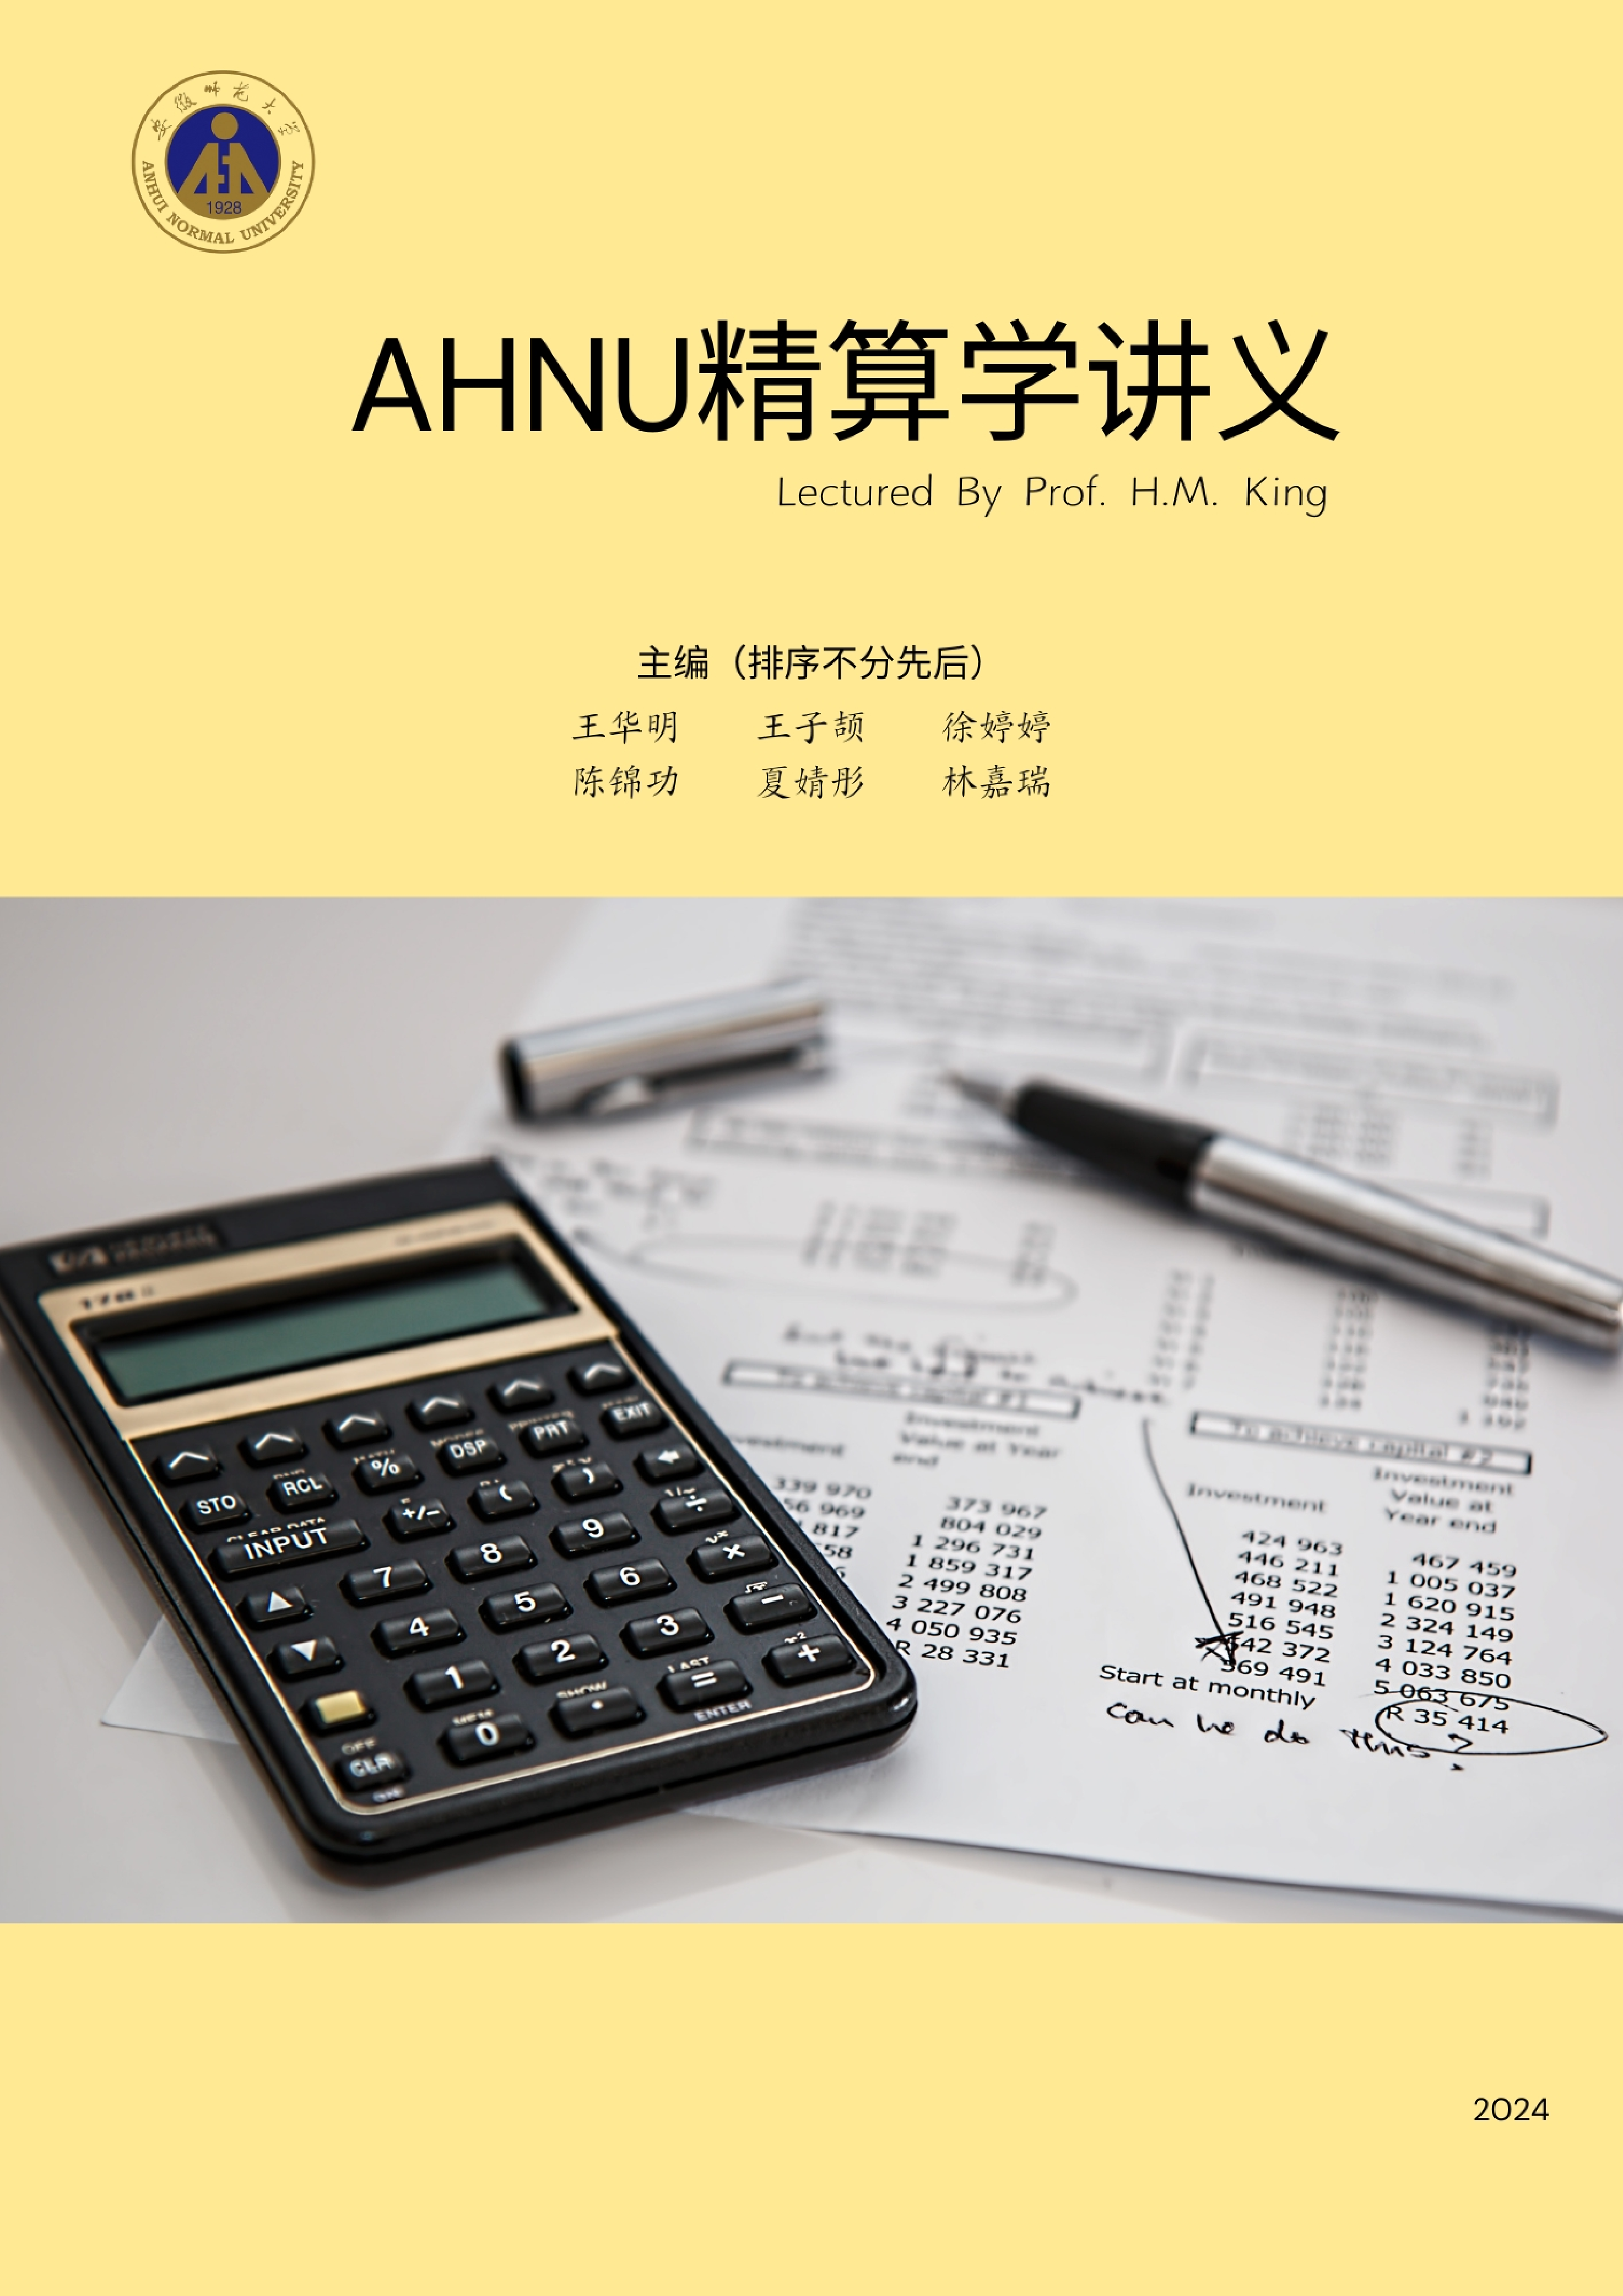
\includepdf{PDFCover.pdf}

%\large
\title{\Huge\textbf{《精算学》讲义}}

\author{{\large 王华明}\thanks{\large 安徽师范大学数学与统计学院, 安徽芜湖(241003).  Email:hmking@ahnu.edu.cn}}
\date{}
\maketitle
\newpage
\thispagestyle{empty}
\large

\newpage
\frontmatter


\addcontentsline{toc}{chapter}{序}
 \begin{center}
    \begin{minipage}[c]{12cm}
        \begin{center}\textbf{\Large 序}\quad \end{center}
        \vspace{-0em} \hspace{2em} { 本讲义是王华明老师在2023-2024年第2学期讲授的《精算学》课程笔记的电子版. 授课对象包括安徽师范大学2021级统计学专业全体同学及少数几位跨专业选课的同学. 教材选用的是北京大学出版社的《寿险精算基础》一书, 该书的作者是杨静平教授. 在此对北京大学出版社及杨静平教授表示感谢.}
    \end{minipage}
\end{center}
\newpage
\addcontentsline{toc}{chapter}{精算学内容}
\begin{center}
    {\bf\hei\Large 精算学内容}
\end{center}
\begin{enumerate}
    \item 你能活多久?(生存分布)
    \item 你死的时候, 保险公司支付你1元, 这1元的现值为多少?(人寿保险)
    \item 在你活着时, 保险公司每年支付你1元, 这些支付的现值是多少?(生存年金)
    \item 上述的寿险与生存年金, 你该向保险公式缴纳多少保费?(保费理论)
    \item 保险公司为了保证支付, 要准备多少钱?(准备金理论)
\end{enumerate}

\newpage
\addcontentsline{toc}{chapter}{精算学拓展训练作业}
\begin{center}
  {\bf\Large \heiti 精算学拓展训练作业}

\end{center}
\vspace{.5cm}


{\large
为了巩固精算学的基础知识并进一步了解精算学的研究前沿, 作为课程考核内容之一,
精算学需要提交一份``拓展训练作业", 以下简称大作业. {\red\bf 大作业需在 在6月20日前上交}, 采用手写版(纸质版)或电子版(打印版)都行. 如果是纸质版直接交给我, 如果是电子版, 请通过QQ传给我. 交大作业时不要忘记写上自己的姓名和学号.

\vspace{.3cm}

{\bf\heiti 大作业可以采取以下一些形式:}
\begin{itemize}
  \item[{\bf1.}] 如果你将来有可能从事统计学或者数学研究工作, 请在国内外精算学相关期刊上下载一篇你感兴趣的和精算学相关的论文, 阅读之后, 写一篇读书报告. 国外比较知名的精算学期刊有Insurance: Mathematics and Economics、 ASTIN Bulletin-The Journal of The International Actuarial Association、 Scandinavian Actuarial Journal、 North American Actuarial Journal 等等. 国内精算学相关期刊有《应用概率统计》、《统计与精算》、《精算通讯》等等.

      \item[{\bf2.}] 如果你决定采用第一种方式完成大作业, 满怀激情地下载了一篇精算学相关的论文, 但发现太难了, 很难读懂, 写不出一篇像样的读书报告, 感觉到一种乘兴而来败兴而归的沮丧,  你可以节选论文中相对比较完整的部分内容, 将原文进行翻译, 作为大作业. 如果是原文是中文, 则翻译成英文; 如果原文是英文, 则翻译成中文. 大作业上需包含原文和译文, 以便我对照检查翻译是否正确.


\item[{\bf3.}] 如果你觉得前两种方式太麻烦, 而且你也不打算考研究生, 你也可以选择精算学教材上的一个或者几个知识点, 深入学习, 然后写一篇学习总结交给我. 这种方式无疑对期末考试会有一定帮助, 所以也是很好的选择.

\item[{\bf4.}] 如果你有自己的想法, 想到其他特别的方式完成大作业, 只要大作业的内容和精算学紧密相关, 也行.
\end{itemize}


}

\tableofcontents
\mainmatter

\chapter{生存分布}
\section{新生儿的生存分布}
\begin{itemize}
    \item[{\bf\hei 一.}]{\bf\hei 生存函数}
\end{itemize}

设有一个新生儿, 其寿命记为$X,$ 则$X$是一个非负随机变量. 假设$X$为一个连续型随机变量, 其分布函数为$F_X(x),$ 密度函数为$f_X(x).$ 回忆一下, 我们有 $F_X(x)=\int_0^x f_X(t)dt$ 且在$f_X(x)$的连续点上有
$$F_X'(x)=f_X(x).$$
如下我们总假设密度函数$f_X(t)$连续.
\begin{definition}
    称$s(t):=P(X>t),t>0$ 为$X$的生存函数.
\end{definition}
易知
\begin{align}\label{sf}
    s(t)=1-F_X(t), s'(t)=-f_X(t).
\end{align}

\begin{itemize}
    \item[{\bf\hei  二.}]{\bf\hei 死亡力}
\end{itemize}

现欲刻画一个$t$时刻还活着的个体瞬间死去的可能性, 做如下计算:

\begin{align}\label{swl}
    \lim_{h\downarrow0} & \frac{P(t<X\le t+h|X>t)}{h}=\lim_{h\downarrow0} \frac{P(t<X\le t+h)}{hP(X>t)}\no                                            \\
                        & =\lim_{h\downarrow0}\frac{P(X\le t+h)-P(X\le t)}{hP(X>t)}=\lim_{h\downarrow0}\frac{F_X(t+h)-F_X(t)}{h}\frac{1}{1-F_X(t)}\no \\
                        & =\frac{F_X'(t)}{1-F_X(t)}=\frac{f_X(t)}{1-F_X(t)}=-\frac{s'(t)}{s(t)}.
\end{align}

\begin{definition}
    称$\mu(t):=-\frac{s'(t)}{s(t)},t\ge 0$ 为新生儿的死亡力函数.
\end{definition}
由\eqref{swl}中的计算可知, 死亡力$\mu(t)$刻画了新生儿在$t$附近死去的``快慢".

\begin{proposition} 关于$\mu(t),$ $s(t)$ 及 $f_X(t)$ 有如下结论:

    {\rm\bf(i)} $\mu(t)=-\frac{s'(t)}{s(t)}=\frac{f_X(t)}{1-F_X(t)}=\frac{f_X(t)}{s(t)};$

    {\rm\bf(ii)} $f_X(t)=\mu(t)s(t);$

    {\rm\bf(iii)} $s(t)=e^{-\int_0^t\mu(s)ds}.$

\end{proposition}
\proof (i)和(ii)可由死亡力$\mu(t)$的定义及(1)式直接得出. 现证明(iii). 注意到$s(0)=P(X>0)=1$ 及
$$\mu(t)=-\frac{s'(t)}{s(t)}=-[\ln s(t)]'.$$ 所以有
$$\ln s(t)=-\int_0^t\mu(s)ds.$$ 故$s(t)=e^{-\int_0^t\mu(s)ds},$ (iii) 得证. \qed


\begin{remark}
    \begin{enumerate}
        \item[{\bf(a)}] 由$s(t) = e^{-\int_{0}^{t}\mu(s)\mathrm{d}s}$ 及$ \mu(t) = -\frac{s'(t)}{s(t)}$可知, 生存函数$s(t)$与死亡力函数$\mu(t)$相互唯一确定.
        \item[{\bf(b)}] 一个函数$\mu(t)$要作为死亡力, 必须满足以下两条:
            \begin{enumerate}
                \item[ $ 1^\circ$] $\mu(t) \geq 0, ~\forall t \geq 0$ (保证$s(t)$单调递减).
                \item[$2^\circ$] $\int_0^{\infty}\mu(t)\mathrm{d}t = \infty$(保证$s(\infty)=0$).
            \end{enumerate}
    \end{enumerate}

\end{remark}




\begin{example}
    假设新生儿的寿命服从以$\lambda$为参数的指数分布, 则密度函数$f_X(t)=\lambda e^{-\lambda x},x>0.$ 分布函数$F_X(t)=\int_0^t f_X(s)ds=1-e^{-\lambda t}, t>0.$ 生存函数$s(t)=1-F_X(t)=e^{-\lambda t},t>0.$  故其死亡力函数为
    \begin{align}\label{ep}
        \mu(t)=-\frac{s'(t)}{s(t)}=-\frac{-\lambda e^{-\lambda t}}{e^{\lambda t}}\equiv\lambda.
    \end{align}
\end{example}

\begin{remark}
    由\eqref{ep}式可知, 若新生儿寿命服从以$\lambda$ 为参数的指数分布, 则死亡力$\mu(t)\equiv \lambda,$ 和$t$ 无关. 这表示新生儿的死亡力在任何时候都是一样的. 也就是说, 新生儿永远年轻. 这当然与实际情况不符. 所以, 指数分布作为寿命分布是有缺陷的. 但由于指数分布的计算较为简单, 所以在理论研究中, 学者们很多时候都采用指数分布作为寿命分布.
\end{remark}
\begin{itemize}
    \item[{\bf\hei 三.}]{\hei\bf 整数年龄与分数年龄}
\end{itemize}
很多时候, 保险金都是在整数时刻支付的. 所以有必要研究整数年龄和分数年龄. 设$K(0)$为$X$的整数部分, $S(0)$为$X$ 的分数部分. 即
$$X = K(0) + S(0).$$
记$\mathring{e}_0 = E(X),$ 它表示新生儿的期望寿命; 记$e_0 = E(K(0)),$ 它表示期望整数寿命. 易知
\begin{equation*}
    e_0 \le \mathring{e}_0 < e_0 + 1.
\end{equation*}

\begin{lemma}\label{lemm0}
    设随机变量$X$的$n$阶矩存在, 即$E(X^n) < \infty,$ 则$\lim_{M \rightarrow \infty}M^ns(M) = 0.$
\end{lemma}
\begin{proof} 注意到
    \begin{align}
        E(X^n)=\int_{0}^\infty s^n f_X(s)ds=\int_0^Ms^n f_X(s)ds +\int_{M}^\infty s^n f_X(s)ds.
    \end{align}
    因$X$的$n$阶矩存在, 故上式左右两端都是有限的. 由于 $\lim_{M\rto} \int_0^Ms^n f_X(s)ds=E(X^n),$ 所以
    $\lim_{M\rto}\int_{M}^{\infty} s^nf_X(s)\mathrm{d}s=0.$ 于是
    \begin{align}
        M^n s(M) & = M^nP(X>M)
        =    \int_{M}^{\infty} M^nf_X(s)\mathrm{d}s  \no                                 \\
                 & \leq \int_{M}^{\infty} s^nf_X(s)\mathrm{d}s \rightarrow 0,\ M\rto.\no
    \end{align}
    引理证毕. \qed
\end{proof}

\begin{proposition}如下结论成立:
    \begin{enumerate}
        \item[(1)] $\mathring{e}_0 = E(X) = \int_0^{\infty}s(t)\mathrm{d}t;$
        \item[(2)] $E(X^2) = \int_{0}^{\infty} 2ts(t)\mathrm{d}t;$
        \item[(3)] $E(K(0)^2) = \sum_{n = 1}^{\infty} (2n-1)s(n);$
        \item[(4)] $e_0=E(K(0)) = \sum_{n = 1}^{\infty} s(n).$
    \end{enumerate}
\end{proposition}
\begin{proof}由分部积分公式和引理\ref{lemm0}可知
    \begin{equation*}
        \begin{aligned}
            {E}\left(X^{n}\right) & =\int_0^\infty t^n\mathrm{d}F(t)=\lim_{M\to\infty}\int_0^Mt^n\mathrm{d}F(t)=-\lim_{M\to\infty}\int_0^Mt^n\mathrm{d}s(t) \\
                                  & \left.=-\lim_{M\to\infty}(\left[t^ns(t)\right]\right|_0^M-\int_0^Mnt^{n-1}s(t)\mathrm{d}t)                              \\
                                  & =\lim_{M\to\infty}[-M^ns(M)]+\lim_{M\to\infty}\int_0^Mnt^{n-1}s(t)\mathrm{d}t                                           \\
                                  & =\int_0^\infty nt^{n-1}s(t)\mathrm{d}t.
        \end{aligned}
    \end{equation*}
    故(1)与(2)得证. 下证(3), 由离散型随机变量函数期望的计算公式, 有
    \begin{align*}
        E(K(0)^2) & = \sum_{k = 0}^{\infty} k^2P(K(0) = k)
        = \sum_{k = 0}^{\infty} k^2[P(X \geq k) - P(X \geq k+1)]                                                            \\
                  & = \sum_{k = 0}^{\infty} k^2s(k) - \sum_{k = 0}^{\infty} k^2s(k+1)                                       \\
                  & =\sum_{k = 0}^{\infty} k^2s(k) - \sum_{k = 0}^{\infty} (k+1)^2s(k+1)+\sum_{k = 0}^{\infty} (2k+1)s(k+1) \\
                  & = \sum_{k = 0}^{\infty} (2k+1)s(k+1)                              = \sum_{n = 1}^{\infty} (2n-1)s(n).
    \end{align*}
    故(3)得证. 类似可证(4). \qed
\end{proof}

\section{$x$岁个体的生存分布}

\begin{itemize}
    \item[{\bf\hei 一.}]{\bf\hei $x$岁个体余命的分布、密度及生存函数}
\end{itemize}

为了方便, 今后将一个$x$岁还活着的个体记为$(x).$ 个体$(x)$的余命记为$T(x).$ 显然有
$$T(x)=X-x.$$
这里特别强调一下,
$T(x)$的分布表示在已知事件$\{X>x\}$发生的条件下, $X-x$的分布. 如果新生儿在$x$岁之前死了, 也就没有了所谓的个体$(x),$ 其余命也就无从谈起.

记$F_{T(x)}(t)$为$T(x)$的分布函数, 则
\begin{align}\label{ft}
    F_{T(x)}(t) & = P(T(x) \leq t|X > x)
    = P(X- x \leq t | X > x)\no                        \\
                & = \frac{P(x<X \leq t + x)}{P(X > x)}
    = \frac{P(X > x) - P(X > x + t)}{P(X > x)}\no      \\
                & = 1 - \frac{s(x+t)}{s(x)}.
\end{align}
记$f_{T(x)}(t)$为$T(x)$的密度函数, 则
\begin{equation}\label{ftd}
    f_{T(x)}(t) = F_{T(x)}'(t) = -\frac{s'(x+t)}{s(x)} = \frac{f_X(x+t)}{s(x)}.
\end{equation}
\begin{definition}
    称$s_{T(x)}(t): = P(T(x)>t)$为个体 $(x)$的的生存函数.
\end{definition}

由\eqref{ft}可得
\begin{align}\label{stf}
    s_{T(x)}(t)=1-F_{T(x)}(t)=\frac{s(x+t)}{s(x)} \text{ 且 }\  s_{T(x)}'(t)=-f_{T(x)}(t).
\end{align}


\begin{itemize}
    \item[{\bf\hei 二.}]{\bf\hei $x$岁个体的死亡力}
\end{itemize}
为了解个体$(x)$在$x+t$岁附近死去的``快慢", 考虑极限

\begin{align*}
    \lim_{\Delta t\to0+} & \frac{P(t<T(x)\leqslant t+\Delta t|T(x)>t)}{\Delta t}
    =  \lim_{\Delta t\to0+}\frac{P(t<T(x)\leqslant t+\Delta t)}{\Delta tP(T(x)>t)}                                          \\
                         & = \lim_{\Delta t\to0+}\frac{s_{T(x)}(t) - s_{T(x)}(t + \Delta t)}{\Delta t}\frac{1}{s_{T(x)}(t)}
    = - \frac{s_{T(x)}'(t)}{s_{T(x)}(t)}                                                                                    \\
                         & = - \frac{\frac{s'(x+t)}{s(x)}}{\frac{s(x+t)}{s(x)}}
    =  -\frac{s'(x+t)}{s(x+t)} = \mu(x+t).
\end{align*}

\begin{definition}
    称$\mu_x(t) = -\frac{s_{T(x)}'(t)}{s_{T(x)}(t)}$为$x$岁个体在$t$年后的死亡力函数.
\end{definition}

\begin{proposition}\label{p21} 我们有

    {\bf(i)} $s_{T(x)}(t)=1-F_{T(x)}(t)=\frac{s(x+t)}{s(x)};$

    {\bf(ii)} $\mu_{x}(t)=\frac{f_{T(x)}(t)}{1-F_{T(x)}(t)}=\frac{f_{T(x)}(t)}{s_{T(x)}(t)}=-\frac{s_{T(x)}'(t)}{s_{T(x)}(t)}.$

    {\bf(iii)} $f_{T(x)}(t)=s_{T(x)}(t)\mu_{x}(t);$

    {\bf(iv)} $\mu_x(t)=\mu(x+t);$

    {\bf(v)} $s_{T(x)}(t)=e^{-\int_0^t \mu_x(s)ds}=e^{-\int_0^t \mu(x+s)ds}=e^{-\int_x^{x+t} \mu(s)ds}.$

\end{proposition}
\proof 利用\eqref{ft}, \eqref{ftd} 和 \eqref{stf}, 很容易证明 (i), (ii), (iii). 下证(iv). 由(ii), \eqref{ftd} 及\eqref{stf} 可得,
\begin{align*}
    \mu_{x}(t)=\frac{f_{T(x)}(t)}{s_{T(x)}(t)}=\frac{f_{X}(x+t)/s(x)}{s(x+t)/s(x)}=\frac{f_{X}(x+t)}{s(x+t)}=\mu(x+t).
\end{align*}
其中, 为了得到最后一个等号, 我们用了命题1.1中的第一条. (iv)得证.

最后证明(v). 注意到$s_{T(x)}(0)=P(T(x)>0)=1$ 且由第(ii)条有
$$\mu_{x}(t)=-\frac{s_{T(x)}'(t)}{s_{T(x)}(t)}=-[\ln s_{T(x)}(t)]'.$$
故 $\ln s_{T(x)}(t)=-\int_0^t\mu_x(s)ds.$ 从而
$s_{T(x)}(t)=e^{-\int_0^t\mu_x(s)ds}.$ 又因为$\mu_x(t)=\mu(x+t),$ 故
\begin{align*}
    s_{T(x)}(t)=e^{-\int_0^t\mu_x(s)ds}=e^{-\int_0^t\mu(x+s)ds}=e^{-\int_x^{x+t} \mu(s)ds},
\end{align*}
其中, 为得到最后一个等号, 我们用定积分的换元法即可. \qed


\begin{remark}
    理论上, 一个人一旦出生, 其死亡力就``注定"了. 如果他在$x$岁还活着, 在$t$ 年后他变为$x+t$ 岁, 此时他的死亡力是$\mu_x(t).$ 换一种观点, 如果站在0 时刻(他出生时)看, 他在$x+t$岁的死亡力应为$\mu(x+t).$ 故有
    $$\mu_x(t)=\mu(x+t).$$
\end{remark}

\begin{example}
    设新生儿的寿命服从以$\lambda>0$为参数的指数分布. 则
    $s(t)=e^{-\lambda t}, t>0.$ 从而有
    \begin{align*}
         & F_{T(x)}(t)=1-\frac{s(x+t)}{s(x)}=1-\frac{e^{-\lambda(x+t)}}{e^{-\lambda x}}=1-e^{-\lambda t} =F_X(t); \\
         & f_{T(x)}(t)=F_{T(x)}'(t)=F_X'(t)=f_X(t);                                                               \\
         & \mu_x(t)=\mu(x+t)\equiv\lambda.
    \end{align*}
    以上计算再次表明, 在指数分布寿命假设下, 新生儿的的寿命$X$与$x$岁的个体的余命$T(x)$的分布相同. 进一步说明指数分布作为寿命分布是有缺陷的.
\end{example}


\begin{proposition}$\forall u,t>0,$ 有
    \begin{align}
         & P(T(x)>t+u|T(x)>t)=P(T(x+t)>u).\label{tu}
    \end{align}
    该式的含义为: 一个$x$岁的人, 在$x+t$岁还活着的条件下, 再活$u$年不死的概率与一个$x+t$ 岁的人在$u$年内未死的概率相等.
\end{proposition}

\proof 对$u,t>0,$ 由条件概率定义知
\begin{align*}
    P(T(x) & >t+u|T(x)>t)=\frac{P(T(x)>t+u)}{P(T(x)>t)}=\frac{P((X-x)>t+u)}{P((X-x)>t)} \\
           & =\frac{P(X-(x+t)>u)}{P(X>x+t)}=  P(X-(x+t)>u|X>x+t)                        \\
           & =P(T(x+t)>u)=\frac{P(T(x)>t+u)}{P(T(x)>t)}.
\end{align*}
命题证毕. \qed

\begin{remark}由\eqref{tu}式立即可得
    \begin{align}\label{tul}
         & P(T(x)\leq t+u|T(x)>t)=P(T(x+t)\leq u).
    \end{align}
\end{remark}
\begin{example}
    设新生儿的寿命服从指数分布, 参数为$\lambda$, 则$\mu(t)\equiv\lambda,$
    \begin{align*}
         & s(t)=e^{-\lambda t},t>0.                                                                                       \\
         & F_{T(x)}=1-\frac{s(x+t)}{s(x)}=1-e^{- \lambda t}=F_x(t).                                                       \\
         & f_{T(x)}(t)=F_{T(x)}(t)=\lambda e^{- \lambda t}=f_x(t),t>0.                                                    \\
         & s_{T(x)}(t)=\frac{s(x+t)}{s(x)}=e^{-\lambda t}=s(t),t>0.                                                       \\
         & \mu_x(t)=\mu(x+t)\equiv\mu,t>0.                                                                                \\
         & e_x = \sum_{k=1}^{\infty} {_kp_x}=\sum_{k=1}^{\infty} {e^{- \lambda t}}=\frac{e^{- \lambda}}{1-e^{- \lambda}}. \\
         & \mathring{e}_x=\int_{0}^{\infty}{_tp_x}dt=\int_{0}^{\infty}{e^{- \lambda t}}dt=\frac{1}{\lambda}.
    \end{align*}
    显而易见, 这里的$\mathring e_x $和$e_x$与$x$无关, 也就是说,  所有人的剩余寿命的期望都是一样的, 和他现在的年龄无关. 这进一步说明指数分布作为寿命分布是有缺陷的.   此外, 因$\mathring{e}_x=ET(x)=\frac{1}{\lambda},$ 故指数分布的参数$\lambda$正好是期望寿命的倒数.
\end{example}

\begin{itemize}
    \item[{\bf\hei 三.}]{\bf\hei 一些精算学表示法}
\end{itemize}
注意到 $ s_{T(x)}(t)=P(T(x)>t)$表示个体$ (x)$在$t$年后还活着的概率; 而$F_{T(x)}(t)=P(T(x)\le t)$ 表示个体$(x)$在$t$ 年内死去的概率. 这些记号都很复杂, 书写比较困难. 故精算学中需引入一些简单的记号.


定义如下几个记号:
\begin{enumerate}
    \item[$\mathring 1.$] 用$_tp_{x}\stackrel{\text{def}}{=}P(T(x)>t)=s_{T(x)}(t)$
        表示个体$(x)$在$t$年后还活着的概率. 显然有
        $$ {}_tp_x=s_{T(x)}(t)=\mathrm{e}^{-\int_{0}^{t}\mu_x(s)\mathrm{d}s}=\mathrm{e}^{-\int_{0}^{t}\mu(x+s)\mathrm{d}s}=\mathrm{e}^{-\int_{x}^{x+t}\mu(s)\mathrm{d}s}.$$
    \item[$\mathring 2.$] 用$_tq_{x}\stackrel{\text{def}}{=}P(T(x)\leq t)=F_{T(x)}(t)$
        表示一个$x$岁的人在$t$年内死亡的概率. 易知
        $$_tp_{x}+{}_tq_{x}=1.$$
    \item[$\mathring 3.$] 用$ _{u|t}q_x=P(u<T(x)\leq u+t)$
        表示一个$x$岁的人在$x+u$岁还活着, 但在未来$t$年内死亡的概率.
\end{enumerate}
\begin{proposition}如下几个结论成立:

    (i) $\frac{d(_tp_x)}{dt}=-_tp_x\mu_x(t);$

    (ii) $\frac{d(_tp_x)}{dx}= {}_tp_x(\mu(x)-\mu(x+t)).$


\end{proposition}

\proof (i) 注意到${}_tp_x=\mathrm{e}^{-\int_{0}^{t}\mu_x(s)ds}.$ 故
$$\frac{d(_tp_x)}{dt}=\frac{d(\mathrm{e}^{-\int_{0}^{t}\mu_x(s)ds})}{dt}=\mathrm{e}^{-\int_{0}^{t}\mu_x(s)ds}\z({-\int_{0}^{t}\mu_x(s)ds}\y)^{\prime}_t=-_tp_x\mu_x(t).$$

(ii) 利用等式${}_tp_x=e^{-\int_{x}^{x+t}\mu_x(s)ds},$ 有
$$\frac{d(_tp_x)}{dx}=\z(e^{-\int_{x}^{x+t}\mu_x(s)ds}\y)^{\prime}_x=e^{-\int_{x}^{x+t}\mu(s)ds}\z({-\int_{x}^{x+t}\mu(s)ds}\y)^{\prime}_x= {}_tp_x(\mu(x)-\mu(x+t)).$$
命题证毕.
\qed

\begin{proposition}以下结论成立:

    (1) $f_{T(x)}(t)={}_tp_x\cdot \mu_x(t);$

    (2) $_tp_x={}_sp_x\cdot{}_{t-s}p_{x+s},0\leq s\leq t;$

    (3) ${}_{u|t}q_x={}_up_x-{}_{u+t}p_x, u,t>0;$

    (4) ${}_{u|t}q_x={}_up_x~{}_{t}q_{x+u},u,t\ge0.$
\end{proposition}
\proof (1)是显然的, 不需证明. (2)
固定$0\le s\le t,$ 则由条件概率性质可知
\begin{align*}
    {}_tp_x & =P(T(x)>t)=P(T(x)>s)P(T(x)>t|T(x)>s) \\
            & ={}_sp_xP(T(x)>t+s-s|T(x)>s)         \\
            & ={}_sp_xP(T(x+s)>t-s)                \\
            & ={}_sp_x\cdot{}_{t-s}p_{x+s}.\end{align*}

(3) 对$t,u\ge0,$ 简单计算可知
\begin{align*}
    {}_{u|t}q_x & =P(u<T(x)\leq u+t)                          \\
                & =P(T(x)>u)-P(T(x)>u+t)={}_up_x-{}_{u+t}p_x.
\end{align*}

(4) 固定$t,u\ge0,$ 利用\eqref{tul}得
\begin{align*}
    {}_{u|t}q_x & =P(u<T(x)\leq u+t)=P(T(x)>u)P(T(x)\leq u+t|T(x)>u) \\
                & ={}_up_xP(T(x+u)<t)= {}_up_x{}~_{t}q_{x+u}.
\end{align*}
命题证毕. \qed

\begin{itemize}
    \item[{\bf\hei 四.}]{\bf\hei 个体$(x)$的整数与分数余命}
\end{itemize}
类似处理新生儿的寿命一样, 可将个体$(x)$的余命$T(x)$分为整数部分和小数部分.
设
\begin{align*}
     & T(x)=K(x)+S(x),
\end{align*}
其中$K(x)$是$T(x)$的整数部分, $S(x)$是$T(x)$的小数部分. 记
\begin{align*}
     & \mathring{e}_x\stackrel{\text{def}}{=}E(T(x)), \   {e_x}\stackrel{\text{def}}{=}E(K(x)).
\end{align*}
则简单计算可知 \begin{align*}
    \mathring{e}_x & =E(T(x))=\int_{0}^{\infty}P(T(x)>t)d t=\int_{0}^{\infty}{_tp_xdt};                          \\
    {e_x}          & =E(K(x))=\sum_{k=0}^{\infty}kP(K(x)=k)                                                      \\
                   & =\sum_{k=0}^{\infty}k[P(T(x)\geq k)-P(T(x)\geq k+1)]                                        \\
                   & =\sum_{k=0}^{\infty}k\cdot{}_kp_x-\sum_{k=0}^{\infty}k\cdot{}_{k+1}p_x=\sum_{k=0}^{\infty}{_{k+1}p_x} \\
                   & =\sum_{k=1}^{\infty}{_kp_x}.
\end{align*}

\section{随机生存群}
\begin{itemize}
    \item[{\bf\hei 一.}]{\bf\hei 模型描述}
\end{itemize}

设0时刻系统中有$l_0$个新生儿, 他们的寿命独立同分布, 服从某分布, 生存函数为$s(t),t\ge 0.$  记

$\mathscr{L}(x)$ 为在$x$ 岁还活着的总人数;

$_t \mathscr{D}_x$为$[x,x+t]$内死去的总人数.

设系统中初始时刻的$l_0$个人的寿命分别为$X_1,X_2,...,X_n$, 则他们独立同分布, 且
$$P(X_i>t)=s(t), i=1,...,n.$$
显然有
\begin{align*}
     & \mathscr{L}(x)=\sum_{i=1}^{l_0}I_{\{X_{i}\geqslant x\}},\ {}_t\mathscr{D}_x=\sum_{i=1}^{l_0}I_{\{ x\leqslant X_i<x+t\}},
\end{align*}
其中
$
    I_{A}=\left\{\begin{array}{ll}1,&\omega\in A,\\0,&\omega\in A^c\end{array}\right.
$ 为示性函数.

令 \begin{align*}
    l_x     & \overset{def}{=}E(\mathscr L(x)), \text{ 它表示在}x\text{岁还活着的期望人数};         \\
    {}_td_x & \overset{def}{=}E({}_t\mathscr D_x ),\text{ 它表示在}[x,x+t)\text{内死去人数的期望}.
\end{align*}



\begin{itemize}
    \item[{\bf\hei 二.}]{\bf\hei 几个结论}
\end{itemize}

\begin{proposition} 如下结论成立:
    $$l_x=l_0s(x),\ {}_td_x=l_x-l_{x+t}.$$
\end{proposition}
\proof 注意到$E(1_A)=P(A),$ 所以
\begin{align*}
    l_x     & =E(\mathscr{L}(x))=E\z(\sum_{k=1}^{l_0}I_{\{X_k>x\}}\y)                        \\
            & =\sum_{k=1}^{l_0}E(I_{\{X_k>x\}})
    =\sum_{k=1}^{l_0}P(X_k>x)
    =\sum_{k=1}^{l_0}P(X_1>x)                                                            \\
            & =l_0P(X_1>x)=l_0s(x);                                                      \\
    {}_td_x & =E(_t\mathscr{D}_x)=E\z(\sum_{k=1}^{l_0}I_{\{x<X_k\leq x+t\}}\y)               \\
            & =\sum_{k=1}^{l_0}E(I_{\{x<X_k\leq x+t\}})=\sum_{k=1}^{l_0}P(x<X_k\leq x+t) \\
            & =l_0P(x<X_1\leq x+t)=l_0[P(X_1>x)-P(X_1>x+t)]                              \\
            & =l_0s(x)-l_0s(x+t)
    =l_x-l_{x+t}.
\end{align*}
命题得证. \qed

引入$l_x$及${}_td_x$的目的是为了计算生存概率${}_tp_x$与死亡概率${}_tq_x.$
\begin{proposition}\label{prop1.8}如下结论成立:

    (i) ${}_tp_x=\frac{l_{x+t}}{l_x},$  ${}_tq_x=\frac{{}_td_x}{l_x},$  $l_{x+t}=l_xe^{-\int_{x}^{x+t}\mu(s)ds}$

    (ii) $\frac{dl_x}{dx}=-l_x\mu(x),$ $_nd_x=\int_{x}^{x+n}l_y\mu(y)dy.$
\end{proposition}

\proof 我们先证(i). 由$l_x=l_0s(x)$知$s(x)=\frac{l_x}{l_0}$, 所以
$$_tp_x=s_{T(x)}(t)=\frac{s(x+t)}{s(x)}=\frac{l_{x+t}/l_0}{l_x/l_0}=\frac{l_{x+t}}{l_x}.$$
由此可推出\begin{align*}
     & l_{x+t}=l_x\cdot{}_tp_x=l_xe^{-\int_{x}^{x+t}\mu(s)ds};                          \\
     & {}_tq_x=1-{}_tp_x=1-\frac{l_{x+t}}{l_x}=\frac{l_x-l_{x+t}}{l_x}=\frac{_td_x}{l_x}.
\end{align*}

下证(ii). 由(i)知,
$$\frac{dl_x}{dx}=l_0e^{-\int_{0}^{x}\mu(t)dt}(-\mu(x))=l_0s(x)(-\mu(x))=-l_x\mu(x).$$
由此可导出
$${}_nd_x=l_x-l_{x+n}=-\int_{x}^{x+n}\frac{dl_y}{dy}dy=\int_{x}^{x+n}l_y\mu(y)dy.$$
命题证毕.
\qed

\begin{remark} 下面我们分析等式
  ${}_td_x=\int_x^{x+t} l_yu(y)dy$的含义.

分析: 等式左端${}_td_x$表示在$[x,x+t]$内死去的人数. 现分析右端. 注意到$$\mu(y)dy=-\dfrac{s'(y)}{s(y)}dy=-\dfrac{ds(y)}{s(y)}=\dfrac{s(y)-s(y+\Delta y)}{s(y)}.$$ 所以$\mu(y)dy$表示一个人在$y$岁还活着的条件下, 在$[y,y+dy]$内死去的概率, 于是$l_y\mu(y)dy$表示在$[y,y+dy]$内死去的人数. 对$y$积分可知, 等式右端的$\int_x^{x+t}l_y\mu(y)dy$表示在$[x,x+t]$内死去的人数. 所以右端等于左端.
\end{remark}

\section{生命表的元素}
补充知识:

{\rm\bf(i)} 在精算学的诸多记号中, 若左下标是1, 通常将其省略, 例如
$${p_x}\triangleq{}_1p_x,{q_x}\triangleq{}_1q_x,$$
$$L_x\triangleq{}_1L_x,{}_{u|}q_x\triangleq{}_{u|1}q_x.$$

{\rm\bf(ii)} $a\wedge b=\min\{a,b\},\ a\vee b=\max\{a,b\},\ EX=\int_0^{\infty}xf(x)dx,X\ge0.$

下面用两种方法计算$E(X\wedge t).$


法一: 由数学期望的定义, 可知
\begin{align*}
    E(X\wedge t) & =\int_0^{\infty}(x\wedge t)f(x)dx                           \\
                 & =\int_0^t(x\wedge t)f(x)dx+\int_t^{\infty}(x\wedge t)f(x)dx \\
                 & =\int_0^txf(x)dx+\int_t^{\infty}tf(x)dx                     \\
                 & =\int_0^txf(x)dx+tP(X>t).
\end{align*}


法二: 对常数$\mathbf 1$进行分解可得
\begin{align*}
    E(X\wedge t) & =E[(X\wedge t)\mathbf{1}]                                \\
                 & =E((X\wedge t)[I_{X<t}+I_{X\ge t}])             \\
                 & =E((X\wedge t)I_{X<t})+E((X\wedge t)I_{X\ge t}) \\
                 & =E(XI_{X<t})+E(tI_{X\ge t})                     \\
                 & =\int_0^{\infty}xI_{x<t}f(x)dx+tE(I_{X\ge t})   \\
                 & =\int_0^t xf(x)dx+tP(X\ge t).                   \\
\end{align*}


{\rm\bf(iii)} 条件数学期望. 设$A$是一个随机事件, $X$为一个随机变量, 给定事件$A$的条件下, $X$的条件期望定义为
$$E(X|A)\overset{def}{=}\frac{E(XI_A)}{EI_A}=\frac{E(XI_A)}{P(A)}.$$
可以类似条件概率的定义理解条件期望的定义.

有了以下上的准备知识, 下面我们逐一介绍生命表中的元素.

\begin{itemize}
    \item[{\bf\hei 一.}]{\bf\hei ${}_tL_x:$ 所有人在$[x,x+t)$内活过的总时间}
\end{itemize}


一个体$(x)$在$[x,x+t)$内活过的总时间为$T(x)\wedge t$, 这是因为

若$T(x)<t$, 则$(x)$在$[x,x+t)$内活过的时间$T(x).$

若$T(x)\ge t$, 则$(x)$在$[x,x+t)$内活过的时间$t.$

又因为在$x$岁还活着的人有$l_x$个, 故所有人在$[x,x+t)$内活的总时间为$l_x(T(x)\wedge t)$, 记其期望为$$ {}_tL_x=l_xE(T(x)\wedge t).$$
由${}_tL_x$的定义可知, 它表示所有人在$[x,x+t)$内活的总时间的期望.
\begin{proposition} 如下结论成立:
    \begin{align*}
        {}_tL_x & =l_xE(T(x)\wedge t)                 \\
                & =\int_0^t sl_{x+s}\mu(x+s)ds+tl_{x+t} \\
                & =\int_0^tl_{x+s}ds
    \end{align*}
\end{proposition}
\proof 第一个等式是定义. 现证第二个等式. 注意到
\begin{align*}
    {}_tL_x & =l_xE(T(x)\wedge t)                                                                  \\
            & =l_x\int_0^{\infty} (s\wedge t){}_sp_x\mu_x(s)ds                                     \\
            & =\int_0^{\infty}(s\wedge t)l_{x+s}\mu(x+s)ds                                         \\
            & =\int_0^tsl_{x+s}\mu(x+s)ds+\int_t^{\infty}tl_{x+s}\mu(x+s)ds                        \\
            & =\int_0^tsl_{x+s}\mu(x+s)ds+tl_{x+t}\int_t^{\infty}\frac{l_{x+s}}{l_{x+t}}\mu(x+s)ds
\end{align*}

其中,\begin{align*}
    \int_t^{\infty}\frac{l_{x+s}}{l_{x+t}}\mu(x+s)ds
     & =\int_0^{\infty}\frac{l_{x+t+u}}{l_{x+t}}\mu(x+t+u)du \\
     & =\int_0^{\infty}{}_up_{x+t}\mu_{x+t}(u)du             \\
     & =\int_0^{\infty}f_{T{(x+t)}}(u)du                     \\
     & =1.
\end{align*}

于是 , ${}_tL_x=\int_0^tsl_{x+s}\mu(x+s)ds+tl_{x+t}.$ 故第二个等式成立.


下证第三个等式. 注意到
$$dl_y=-l_y\mu(y)dy$$
$$\Rightarrow dl_{x+s}=-l_{x+s}\mu(x+s)ds$$
$$\Rightarrow\int_0^tsdl_{x+s}=-\int_0^tsl_{x+s}\mu(x+s)ds.$$
由此可知$$sl_{x+s}\vert^{t}_{0}-\int_0^tl_{x+s}ds=-\int_0^tsl_{x+s}\mu(x+s)ds.$$
所以
$$\int_0^tsl_{x+s}\mu(x+s)ds+tl_{x+t}=\int_0^tl_{x+s}ds.$$
第三个等式得证.
\qed
\begin{remark}
  表达式$\int_0^tsl_{x+s}\mu(x+s)ds+tl_{x+t}$的含义如下:

\noindent 一方面, 在$x+s$岁活着的人有$l_{x+s}$个, 每个人在$[x+s,x+s+ds]$内死去的概率为$\mu(x+s)ds,$ 所以, 在$[x+s,x+s+ds]$内死去的人数为$l_{x+s}\mu(x+s)ds$, 他们每个人在$[x,x+t]$内活$s$年, 所以在$x+s$岁死去的人在$[x,x+t]$ 内活的总时间为$sl_{x+s}\mu(x+s)ds,$ 再对$s$在$(0,t)$求积分(求和)可知, $\int_0^tsl_{x+s}\mu(x+s)ds$表示在$[x,x+t]$内死去的人在这段时间内活过的总时间.

另一方面, 在$x+t$岁还活着的人有$l_{x+t}$个, 他们每个人在$[x,x+t)$内活了$t$岁, 故他们在$[x,x+t)$内总共活了$tl_{x+t}$岁.

综合以上分析, $\int_0^tsl_{x+s}\mu(x+s)ds+tl_{x+t}$表示所有人在$[x,x+t]$内活过的总时间, 这是一个复杂的公式, 但它有一个简单的表达$\int_0^tl_{x+s}ds.$
\end{remark}


\begin{itemize}
    \item[{\bf\hei 二.}]{\bf\hei $a(x):$ 一个$x$岁的人在1年内死去的条件下, 在$[x,x+1)$内活过的期望时间}
\end{itemize}

个体$(x)$的余命为$T(x)$, 所以$$a(x)=E(T(x)|T(x)\le1).$$
\begin{proposition}以下等式成立:
    $$a(x)=\dfrac {\int_0^1t{}_tp_xu_x(t)dt}{q_x}.$$
\end{proposition}
\proof 利用条件数学期望的定义得
\begin{align*}
    a(x) & =E(T(x)|T(x)\le1)                                                \\
         & =\dfrac {E(T(x)I_{\{T(x)\le1\}})}{P(T(x)\le1)}                   \\
         & =\dfrac {\int_0^{\infty}tI_{\{t\le1\}}f_{T(x)}(t)dt}{q_x}     \\
         & =\dfrac {\int_0^{\infty}tI_{\{t\le1\}}{}_tp_x\mu_x(t)dt}{q_x} \\
         & =\dfrac {\int_0^1t{}_tp_x\mu_x(t)dt}{q_x}.
\end{align*}
命题证毕.\qed

利用$a(x)$可以给出$L_x$的另一个表达式.
\begin{proposition}如下
    等式成立: $$L_x=d_xa(x)+l_{x+1}.$$
\end{proposition}
\proof 由$L_x$的定义可知
\begin{align*}
    L_x & =l_xE(T(x)\wedge1)                                                     \\
        & =l_xE(T(x)\wedge1)I_{\{T(x)<1\}})+l_xE(T(x)\wedge 1)I_{\{T(x)\ge 1\}}) \\
        & =l_xE(T(x)I_{\{T(x)<1\}})+l_xE(I_{\{T(x)\ge 1}\})                   \\
        & =l_xP(T(x)<1)E(T(x)|T(x)<1)+l_xP(T(x)\ge 1)                            \\
        & =l_xq_xa(x)+l_xp_x                                                     \\
        & =d_xa(x)+l_{x+1}.
\end{align*}
证毕. \qed
\begin{remark}
 表达式$L_x=d_xa(x)+l_{x+1}$的含义如下:

\noindent 等式右端的$d_xa(x)$表示$[x,x+1)$内死去的人在$[x,x+1)$内活过的总时间. 右端的$l_{x+1}\times1$ 表示在$x+1$岁活着的$l_{x+1}$人在$[x,x+1)$内活过的总时间. 所以, 右端表示所有人在$[x,x+1)$活过的总时间, 正好等于左端的$L_x.$
\end{remark}

\begin{itemize}
    \item[{\bf\hei 三.}]{\bf\hei ${}_nm_x=\dfrac {{}_nq_x}{\int_0^n{}_tp_xdt}$(中心死亡率)}
\end{itemize}


\begin{proposition}如下结论成立:
    $${}_nm_x=\dfrac{{}_nd_x}{{}_nL_x}.$$
\end{proposition}
\proof 简单计算可得
$${}_nm_x=\dfrac{{}_nq_x}{\int_0^n{}_tp_xdt}=\dfrac{{}_nd_x/l_x}{\int_0^n\dfrac{l_{x+t}}{l_x}dt}=
    \dfrac{{}_nd_x}{{}_nL_x}.$$命题证毕.\qed

\begin{itemize}
    \item[{\bf\hei 四.}]{\bf\hei $T_x\triangleq\int_0^{\infty}l_{x+s}ds={}_{\infty}L_x$}
\end{itemize}
显而易见, $T_x$表示所有人在$[x,\infty)$内活过的总时间.

\begin{itemize}
    \item[{\bf\hei 五.}]{\bf\hei $Y_x\triangleq\int_0^{\infty}T_{x+s}ds.$}
\end{itemize}

生命表中包含$q_x,l_x,d_x,L_x,T_x,\mathring{e}_0$等元素. 总的来说, 利用生命表可以计算出生存概率${}_kp_x,$ 死亡概率${}_kq_x,$ ${}_{k|j}q_x$等.
\newpage

\section{分数年龄上的死亡假设}
\begin{itemize}
    \item[{\bf\hei 一.}]{\bf\hei 为什么引入分数年龄死亡力假设?}
\end{itemize}

如前所述, $_{k}p_{x}=\frac{l_{x+k}}{l_{x}}.$ 若$k$为整数, 可查生命表计算$_{k}p_{x}.$ 例如: $_{2}p_{20}=\frac{l_{22}}{l_{20}}.$

但如果$k$不是整数, 例如, ${}_{2.5}p_{20}=\frac{l_{22.5}}{20},$ 由于$l_{22.5}$生命表中没有给出, 所以无法直接计算${}_{2.5}p_{20}.$


注意到$T(x)=K(x)+S(x),$ 其中$K(x)$是整数部分, $S(x)$是分数部分. 如果知道了分数部分$S(x)$的分布, 就可以计算类似于$l_{22.5}$这样的值.


关于$S(x)$的分布, 我们介绍两个常用的假设:

{\rm\bf(i)} 死亡力均匀分布假设$S(x)\sim U(0,1)$

{\rm\bf(ii)} 常数死亡力假设.

\begin{itemize}
    \item[{\bf\hei 二.}]{\bf\hei 死亡力均匀分布假设(UDD假设)}
\end{itemize}

{\rm\bf1.} 定义: 若$x$为非负整数, $s(t)$是生存函数, 若$\forall t\in [0,1),$ 都有
\begin{align}\label{tula}
     & s(x+t)=(1-t)s(x)+ts(x+1).
\end{align}

称在$[x,x+1)$上, 死亡力均匀分布假设成立.

{\rm\bf2.} 设$[x,x+1)$上UDD假设成立, 则有以下结论:
\begin{enumerate}
    \item[$\mathring 1.$] $l_{x+t}=(1-t)l_{x}+tl_{x+1},t\in [0,1).$

        \proof 由UDD假设的定义, \begin{align*}
            l_{x+t} & =l_{0}s(x+t)                 \\
                    & =l_{0}(1-t)s(x)+l_{0}ts(x+1) \\
                    & =(1-t)l_{x}+tl_{x+1}.
        \end{align*}
        证毕.\qed
    \item[$\mathring 2.$] $_{t}d_{x}=td_{x},t\in [0,1).$

 \proof
利用第一个结论可得
       \begin{align*}
            _{t}d_{x} & =l_{x}-l_{x+t}             \\
                      & =l_x-(1-t)l_{x}-tl_{x+t}   \\
                      & =t(l_{x}-l_{x+1}) =td_{x}.
        \end{align*}
        证毕.\qed
    \item[$\mathring 3.$] $_{t}q_{x}=tq_{x},t\in [0,1).$

        \proof 利用第二个结论可知, \begin{align*}
            _{t}q_{x} & =\frac{_{t}d_{x}}{l_{x}} =\frac{td_{x}}{l_{x}}  = tq_{x}.
        \end{align*}
        证毕.\qed
    \item[$\mathring 4.$] $f_{T(x)}(t)=q_{x},t\in [0,1).$

        由该结论可以看出, 死亡力均匀分布假设下, 个体在$[x,x+1)$内死亡的条件下, $T(x)$在$[0,1)$内的密度函数是一个常数. 也就是$S(x)$服从均匀分布.

        \proof 由第三个结论直接可得\begin{align*}
            f_{T(x)}(t) & =\frac{d(_{t}q_{x})}{dt} =\frac{d(tq_{x})}{dt} =q_x.
        \end{align*}
        证毕.\qed
    \item [$\mathring 5.$] $\mu_{x}(t)=\frac{q_{x}}{1-tq_x}$

          \proof 基于第四个结论, 我们有\begin{align*}
              \mu_{x}(t) & =\frac{f_{T(x)(t)}}{s_{T(x)}(t)} =\frac{q_{x}}{_{t}p_{x}} =\frac{q_{x}}{1-{}_{t}q_{x}} =\frac{q_{x}}{1-tq_{x}}.
          \end{align*}
          证毕.\qed
\end{enumerate}

{\rm\bf3.} 在UDD假设之下, 我们有如下两个命题:

 \begin{proposition}\label{p1.13}已知在每一年龄年上UDD假设成立, 则$K(x)$与$S(x)$相互独立, 且$S(x)$ 服从
 $[0,1]$上的均匀分布.
\end{proposition}
\proof
考虑条件概率$P(S(x) \leq t \mid K(x) = k)$, 有
\begin{align*}
    P(S(x) \leq t \mid K(x) = k) & = \frac{P(S(x) \leq t, K(x) = k)}{P(K(x) = k)}                                                                          \\
                                 & = \frac{_{k|t}q_{x}}{_{k|}q_{x}} = \frac{_{k}p_{x}\,_{t}q_{x+k}}{_{k}p_{x}\,q_{x+k}} = \frac{_{t}q_{x+k}}{q_{x+k}} = t.
\end{align*}
因此, $K(x)$与$S(x)$相互独立, 且$S(x)$服从$[0,1]$上的均匀分布. 证毕.\qed

\begin{proposition}在每一年龄年UDD假设成立时, 有
    $$\mathring{e}_{x}=e_{x}+\frac{1}{2},\   D(T(x))=D(K(x))+\frac{1}{12}.$$
\end{proposition}
\proof
根据命题\ref{p1.13}的结果可知, $K(x)$与$S(x)$相互独立, 且$S(x)$服从$[0,1]$上的均匀分布. 因此有
\begin{align*}
    \mathring{e}_{x} & =E(K(x)+S(x))        \\
                     & = E(K(x))+E(S(x))    \\
                     & = e_{x}+\frac{1}{2},
\end{align*}
及\begin{align*}
    D(T(x)) & =D(K(x)+S(x))             \\
                     & =D(K(x))+D(S(x)) \\
                     & =D(K(x))+\frac{1}{12}.
\end{align*}
证毕.\qed

\begin{itemize}
    \item[{\bf\hei 三.}]{\bf\hei 常数死亡力假设}
\end{itemize}

{\rm\bf1.}  定义: 设$x$为整数, 若$\forall t\in [0,1)$有
\begin{align}\label{tulb}
    \ln s(x+t)=(1-t)\ln s(x)+t\ln s(x+1).
\end{align}
则称生存函数在年龄段$[x,x+1)$满足\textbf{常数死亡力假设}.

{\rm\bf2.} 常数死亡力假设下的一些结论

 \begin{proposition}设在年龄段$[x,x+1)$常数死亡力假设成立, 则对$t\in (0,1)$, 有
    \begin{enumerate}
        \item[$\mathring 1.$] 期望生存人数满足
            $$\ln l_{x+t}=(1-t)\ln l_{x}+t\ln l_{x+1}.$$
            \proof 因$l_{x}=l_{0}s(x)$, 所以由公式\eqref{tulb}知\begin{align*}
                \ln \frac{l_{x+t}}{l_{0}}=(1-t)\ln \frac{l_{x}}{l_{0}}+t\ln \frac{l_{x+1}}{l_{0}}.
            \end{align*}故$\ln l_{x+t}=(1-t)\ln l_{x}+t\ln l_{x+1},$
            证毕.\qed
        \item[$\mathring 2.$] 死亡力为常数, 即
            $$\mu _{x}(t)=-\ln p_{x}\stackrel{\triangle}{=}\mu;$$
            \proof 对公式\eqref{tulb}取指数得
            \begin{align*}
                                    s(x+t) & =s(x)^{1-t}s(x+1)^{t}                              \\
                \Longleftrightarrow & {}_{x+t}p_{0} = {}_xp_{0}^{1-t}{}_{x+1}p_{0}^t             \\
                \Longleftrightarrow & {}_{x}p_{0}{}_{t}p_x = {}_xp_{0}~p_{x}^{t}                 \\
                \Longleftrightarrow & {}_{t}p_x = p_x^t                                          \\
                \Longleftrightarrow & e^{-\int_{0}^{t}\mu_x(s)ds} = e^{-\int_{0}^{t}-\ln p_x ds}.
            \end{align*}
            于是有$\mu _{x}(t)=-\ln p_{x}$.\qed
        \item[$\mathring 3.$] $$l_{x+t}=l_{x}e^{-\mu t},\ _{t}q_{x}=1-p^{t}_{x},\ f_{T(x)}(t)=-p_{x}^{t}\ln p_{x}.$$
            \proof 简单计算可知\begin{align*}
                 & l_{x+t}=l_{x}e^{-\int_{x}^{x+t}\mu (s)ds}=l_{x}e^{-\mu t};         \\
                 & _{t}q_{x}=1-{}_{t}p_{x}=1-p_{x}^{t}=1-e^{t\ln p_{x}}=1-e^{-\mu t}; \\
                 & f_{T(x)}(t)={}_{t}p_{x}\mu {}_{x}(t)=p_{x}^{t}\mu=\mu e^{-\mu t}.
            \end{align*} 结论得证.\qed
    \end{enumerate}
\end{proposition}

\begin{example}
    设$S(x)=1-\frac{x}{12},\ 0\leq x\leq 12$, $l_{0}$个个体相互独立, 生存函数都是$S(x)$.

    (1) 求$(_{3}\mathscr D _{0},\ _{3}\mathscr D_{3},\ _{3}\mathscr D _{6},\ _{3}\mathscr D _{9})$的联合分布;

    (2) 求这四个随机变量的期望和方差;

    (3) 求它们两两之间的相关系数.
\end{example}

\solution
易知$l_{0}$个人的寿命$X_{1},X_{2},...,X_{l_{0}}\stackrel{\text{i.i.d.}}{\sim}U[0,12]$. 且随机变量满足
\begin{align*}
  &{}_{3}\mathscr D _{0}=\sum^{l_{0}}_{k=1}I_{\{0\leq X_k \leq 3\}};\\
&{}_{3}\mathscr D _{3}=\sum^{l_{0}}_{k=1}I_{\{3\leq X_k \leq 6\}};\\
&{}_{3}\mathscr D _{6}=\sum^{l_{0}}_{k=1}I_{\{6\leq X_k \leq 9\}};\\
&{}_{3}\mathscr D _{9}=\sum^{l_{0}}_{k=1}I_{\{9\leq X_k \leq 12\}}.
\end{align*}

\noindent(1) 令事件$A=\{_{3}\mathscr D _{0}=k_{1},\ _{3}\mathscr D _{3}=k_{2},\ _{3}\mathscr D _{6}=k_{3},\ _{3}\mathscr D _{9}=k_{4}\}$, 若事件$A$发生, 则在$l_{0}$个人中, 有$k_{1}$人
在$[0,3]$内死亡; 有$k_{2}$人在$[3,6]$内死亡; 有$k_{3}$人在$[6,9]$内死亡; 有$k_{4}$人在$[9,12]$内死亡, 其中$k_{1}+k_{2}+k_{3}+k_{4}=l_{0}.$ 从$k_{1}+k_{2}+k_{3}+k_{4}$个人中, 选出$k_{1}$个人在$[0,3]$内死亡, 有$C_{k_{1}+k_{2}+k_{3}+k_{4}}^{k_{1}}$种选法; 从$k_{2}+k_{3}+k_{4}$个人中, 选出$k_{2}$个人在$[3,6]$内死亡, 有$C_{k_{2}+k_{3}+k_{4}}^{k_{2}}$种选法; 从$k_{3}+k_{4}$个人中, 选出$k_{3}$个人在$[6,9]$内死亡, 有$C_{k_{3}+k_{4}}^{k_{3}}$种选法. 于是
$$
    P(A)=\frac{(k_{1}+k_{2}+k_{3}+k_{4})!}{k_{1}!k_{2}!k_{3}!k_{4}!}\cdot {}_{3}q_{0}^{k_{1}}\cdot {}_{3|3}q_{0}^{k_{2}}\cdot {}_{6|3}q_{0}^{k_{3}}\cdot {}_{9|3}q_{0}^{k_{4}}.
$$

\noindent(2) 对于一个二项分布$B(n, p)$, 其期望$E[X] = np$, 方差$\text{Var}(X) = np(1-p)$.

因此, 对于每个随机变量$_{3}\mathscr D_{k}$有

期望 $$E(_{3}\mathscr D_{k}) = \frac{l_0}{4};$$

方差 $$\text{Var}(_{3}\mathscr D_{k}) = l_0 \cdot \frac{1}{4} \cdot \left(1 - \frac{1}{4}\right) = \frac{3l_0}{16}.$$

\noindent(3) 以$_{3}\mathscr D _{0},\ _{3}\mathscr D _{3}$的相关系数为例:
\begin{align*}
    \text{Cov}(_{3}\mathscr D _{0},\ _{3}\mathscr D _{3}) & =E\z({}_{3}\mathscr D _{0}\ _{3}\mathscr D _{3}\y)-E(_{3}\mathscr D _{0})E(_{3}\mathscr D _{3})                                \\
                                                          & =E\z(\sum ^{l_{0}}_{k=1}I_{\{0\leq X_{k}\leq 3\}}\cdot \sum ^{l_{0}}_{j=1}I_{\{3\leq X_{j}\leq 6\}}\y)-\z(\frac{l_{0}}{4}\y)^{2} \\
                                                          & =\sum^{l_{0}}_{k=1}\sum_{j\neq k}E(I_{\{0\leq X_{k}\leq 3\}}\cdot I_{\{3\leq X_{j}\leq 6\}})-\z(\frac{ l_{0}}{4}\y)^{2}      \\
                                                          & =\frac{l_{0}(l_{0}-1)}{16}-\frac{l_{0}^{2}}{16}                                                                          \\
                                                          & =-\frac{l_{0}}{16}.
\end{align*}
(对于$\sum^{l_{0}}_{k=1}\sum_{j\neq k}E(I_{\{0\leq x_{X}\leq 3\}}\cdot I_{\{3\leq X_{j}\leq 6\}}) = \frac{l_{0}(l_{0}-1)}{16}$ 的理解: 其中$\sum^{l_{0}}_{k=1}\sum_{j\neq k}1 = l_0(l_0-1)$, 而$p(I_{c\leq X_{i}\leq c+3}) = \frac14$, 故$I_{0\leq X_{k}\leq 3}$ 与$I_{3\leq X_{j}\leq 6}$同时取1的概率为$\frac{1}{16}$.)

求出协方差后即可求相关系数:
\begin{align*}
    \rho(_{3}\mathscr D _{0},\ _{3}\mathscr D _{3}) & =\frac{\text{Cov}(_{3}\mathscr D_{0},\ _{3}\mathscr D _{3})}{\sqrt{D(_{3}\mathscr D _{0})}\cdot \sqrt{D(_{3}\mathscr D _{3})}} \\
                                                    & =\frac{-\frac{l_{0}}{16}}{\sqrt{\frac{3}{16}l_{0}\cdot \frac{3}{16}l_{0}}}                                                     \\
                                                    & =-\frac{1}{3}.
\end{align*}
类似计算可知, 两两之间所有相关系数皆为$-\frac{1}{3}$.\qed

\section{作业}
\begin{exs}
    某人现年20岁, 假设他的余命$T(20)$服从$[0,60]$ 上的均分分布, 求$F_{T(20)}(t),$ $ f_{T(20)}(t),$ $\mu_{20}(t),$ $s_{T(20)}(t).$
\end{exs}

\begin{exs}
    设$\mu(t)=\frac{1}{(t+e)(\ln (t+e))^a},t\ge0.$ 讨论$a$取何值时, $\mu(t)$可作为死亡力函数, 并求出$s_{T(x)}(t),$ $f_{T(x)}(t).$
\end{exs}

\begin{exs}
    假设新生儿的寿命为$X,$ 死亡力为$\mu(t)=\frac{a}{(t+1)},t\ge0, a>0.$ 讨论$a$何值时, $D(X)$存在并求出$D(X).$
\end{exs}

\begin{exs}
    证明: $\frac{d}{dx}\mathring e_x=\mathring e_x\mu(x)-1.$
\end{exs}

\begin{exs}设系统中有$l_0$个新生儿, 它们的寿命独立同分布, 生存函数为
    $$s(t)=1-\frac{t}{16}, 0\le t\le 16.$$ 证明$$({}_4\mathscr D_0, {}_4\mathscr D_4,{}_{4}\mathscr D_8, {}_{4}\mathscr D_{12})$$服从多项分布, 并计算 (1) 每个随机变量的期望; (2) 每个随机变量的方差; (3) 每两个随机变量的相关系数; (4) 对你计算所得的结果进行简要分析.
\end{exs}

\begin{exs}
    你现在多少岁? 请根据课本303页的附表2.1(男生用)、307页附表2.2(女生用)计算你80岁还活着的概率.
\end{exs}

\begin{exs}
    设$i$为复利率, $\nu=\frac{1}{1+i}$为贴现因子, $\delta=\ln (1+i)$为利息力.

    (1) 设$\mu_{x}(t)\equiv \mu =0.05, \delta\equiv 0.04$,
    求 $$E(\nu^{T(x)}),\ D(\nu^{T(x)}),\ E\z(\int_{0}^{T(x)}\nu^{t}dt\y),\ D\z(\int_{0}^{T(x)}\nu^{t}dt\y)$$.

    (2) 设UDD成立, 求证: $E(\nu^{T(x)})=\frac{i}{\delta}E\z(\nu^{K(x)+1}\y)$.
\end{exs}


\chapter{人寿保险}
\section{人寿保险概述}
\begin{itemize}
    \item[{\bf\hei 一.}]{\bf\hei 人寿保险关心的问题}
\end{itemize}
\begin{enumerate}
    \item 保险金的支付条件, 支付的时刻.
    \item 支付保险金的现值$Z$是多少?
    \item 保险金的精算现值$EZ$.
    \item 风险度量$DZ$.
    \item 精算现值$EZ$, $DZ$的性质.
\end{enumerate}
\begin{itemize}
    \item[{\bf\hei 二.}]{\bf\hei 人寿保险的分类}
\end{itemize}

\begin{equation*}
    \text{人寿保险}
    \begin{cases}
         & \text{生存保险}                                          \\
         & \text{生死合险}                                          \\
         & \text{死亡保险}\begin{cases}
                           & \text{定期死亡保险}                   \\
                           & \text{终身死亡保险}                   \\
                           & \text{延期死亡保险}\begin{cases}
                                 & \text{延期定期死亡保险} \\
                                 & \text{延期终身死亡保险}
                            \end{cases}
                      \end{cases}
    \end{cases}
\end{equation*}

\section{生存保险}
\begin{itemize}
    \item[{\bf\hei 一.}]{\bf\hei 支付方式与支付条件}
\end{itemize}

若被保险人在$n$年内死亡(即$T(x)<n$), 则不予任何支付;

若他在$n$年内未死(即$T(x)\geqslant n$), 则在$n$ 时刻支付他1元保险金.
\begin{itemize}
    \item[{\bf\hei 二.}]{\bf\hei 支付现值$Z$}
\end{itemize}

若$T(x)<n$, 则$Z=0$; 若$T(x)\geqslant n$, 则$Z=1\cdot \nu^n=\nu^n$, 其中贴现因子$\nu=\frac{1}{i+1}.$

即$$Z=\nu^nI_{\left\{ T\left( x \right) \geqslant n \right\}}=\left\{ \begin{array}{ll}
        \nu^n, &\text{若}\,\,T\left( x \right) \geqslant n, \\
        0,&\text{若}\,\,T\left( x \right) <n .           \\
    \end{array} \right.$$
\begin{itemize}
    \item[{\bf\hei 三.}]{\bf\hei 精算现值$EZ$}
\end{itemize}
简单计算可知
\begin{align}
  E\left( Z \right) &=E\left( \nu^nI_{\left\{ T\left( x \right) \geqslant n \right\}} \right)=\nu^nE\left( I_{\left\{ T\left( x \right) \geqslant n \right\}} \right) \no\\ &
    =\nu^nP\left( T\left( x \right) \geqslant n \right) =\nu^n\cdot{}_np_x.\no
\end{align}

$n$年期生存保险的精算现值记为$A_{x:}\overset{1}{{}\annu{n}}$ 或$_nE_x.$
于是有\begin{align}\label{an1}
  A_{x:}\overset{1}{{}\annu{n}} = {}_nE_x=\nu^n\cdot{}_np_x.
\end{align}
\begin{itemize}
    \item[{\bf\hei 四.}]{\bf\hei 二阶矩}
\end{itemize}
易知
$$E\left( Z^2 \right) =E\left( \left[ \nu^nI_{\left\{ T\left( x \right) \geqslant n \right\}} \right] ^2 \right) =E\left( \nu^{2n}I_{\left\{ T\left( x \right) \geqslant n \right\}} \right) =\nu^{2n}\cdot{}_np_x.$$ 故
$$DZ=EZ^2-\left( EZ \right) ^2=\nu^{2n}\cdot{}_np_x\cdot{}_nq_x.$$
\begin{itemize}
    \item[{\bf\hei 五.}]{\bf\hei 精算现值的性质}
\end{itemize}
\begin{proposition}
    $\forall 0\leqslant k\leqslant n$, 有
    \begin{align}\label{1}
        _nE_x={}_kE_x\cdot {}_{n-k}E_{x+k},
    \end{align}
    \begin{align}\label{2}
        (1+i)^k\cdot l_x\cdot{}_nE_x=l_{x+k}\cdot {}_{n-k}E_{x+k}.
    \end{align}
\end{proposition}
\proof 由公式\eqref{an1}可知
$$_nE_x=\nu^n\cdot {}_np_x=\nu^k\cdot \nu^{n-k}\cdot {}_kp_x\cdot {}_{n-k}p_{x+k}={}_kE_x\cdot {}_{n-k}E_{x+k}.$$

利用命题\ref{prop1.8}和\eqref{1}式可得,
$$_nE_x=\nu^k\cdot {}_kp_x\cdot {}_{n-k}E_{x+k}=(\frac{1}{i+1})^k\cdot\frac{l_{x+k}}{l_x}\cdot {}_{n-k}E_{x+k}.$$
故$(1+i)^k\cdot l_x\cdot {}_nE_x=l_{x+k}\cdot {}_{n-k}E_{x+k}.$
\qed


\begin{remark}
    等式$(1+i)^k\cdot l_x\cdot {}_nE_x=l_{x+k}\cdot {}_{n-k}E_{x+k}$ 的含义如下:

    在0时刻, $l_x$个人各自买了一份n年期的生存保险, 保费总额为$l_x\cdot {}_nE_x$, $k$年后, 这笔钱的积累值为$(1+i)^k\cdot l_x\cdot {}_nE_x$,若此时保险公司破产不干了, 他分给在$k$时刻还活着的$l_{x+k}$个人每人${}_{n-k}E_{x+k}$元, 这正好够每个人去重新买一份$n-k$年期的生存保险.
\end{remark}
\section{$n$年期(定期)死亡保险}

一个个体$(x)$投了一份$n$年期死亡保险, 约定: 若$(x)$在$n$年内死亡, 则在其死亡时刻立刻支付$1$元保险金或在其死亡年末支付$1$元保险金. 根据支付时刻的不同, 分以下两种情况讨论:

死亡立即支付——连续型;

死亡年末支付——离散型.
\begin{itemize}
    \item[{\bf\hei 一.}]{\bf\hei 死亡立即支付的$n$年期定期寿险}
\end{itemize}
\begin{itemize}
    \item[{\bf\hei 1.}]{\bf\hei 支付方式和条件}
\end{itemize}

若$(x)$在$n$年内死亡(即$T(x)<n$), 则在$T(x)$时刻支付$1$元保险金;

若$(x)$在$n$年内未死(即$T(x)\geqslant n$), 则不予支付.
\begin{itemize}
    \item[{\bf\hei 2.}]{\bf\hei 支付现值$Z$}
\end{itemize}

若$T(x)<n$, 则$Z=\nu^{T(x)}$; 若$T(x)\geqslant n$, 则$Z=0$.

所以$Z=\nu^{T(x)}I_{\{T(x)<n\}}.$
\begin{itemize}
    \item[{\bf\hei 3.}]{\bf\hei $n$年期定期寿险的精算现值记为$\overline{A}_{x:}^1{}_{{}\annu{n}}$}
\end{itemize}
\begin{remark}
    符号$\overline{A}_{x:}^1{}_{{}\annu{n}}$中, 上划线表示死亡立即支付(连续型), 1表示保险金为
    1元, $x$ 表示被保险人为$x$岁, $n$表示保险期限是$n$年.
\end{remark}

由数学期望的定义立即可得
\begin{align*}
        \overline{A}_{x:}^1{}_{{}\annu{n}}= & EZ=E\left( \nu^{T\left( x \right)}I_{\left\{ T\left( x \right) <n \right\}} \right) =\int_0^{\infty}{\nu^{t}I_{\left\{ t <n \right\}}\cdot f_{T(x)}(t)dt} \\
        =                            & \int_0^{n}{\nu^{t}\cdot {}_tp_x\cdot \mu_{x}(t)dt}=\int_0^{n}{e^{-\delta t}\cdot {}_tp_x\cdot \mu_{x}(t)dt}.
    \end{align*}
\begin{proposition}
    $\forall 0\leqslant k\leqslant n$, 有
    \begin{align}\label{eq2.3}
        \overline{A}_{x:}^1{}_{{}\annu{n}}=\overline{A}_{x:}^1{}_{\annu k}+{}_kE_x\cdot\overline{A}_{x+k:}^1{}\annu{n-k};
    \end{align}
    \begin{align}\label{eq2.4}
        l_x\cdot\overline{A}_{x:\annu{n}}^1=\int_0^{n}{\nu^{t}\cdot l_{x+t}\cdot \mu_{x}(t)dt}.
    \end{align}
\end{proposition}


\proof
先证(\ref{eq2.3})式.
\begin{align*}
    \overline{A}_{x:}^1{}_{\annu{n}} & =\int_0^{n}{\nu^{t}\cdot{}_tp_x\cdot \mu_{x}(t)dt} = \int_0^{k}{\nu^{t}\cdot  _tp_x\cdot \mu_{x}(t)dt} +\int_k^{n}{\nu^{t}\cdot  _tp_x\cdot \mu_{x}(t)dt}                                                     \\
                                & = \overline{A}_{x:}^1{}_{\annu k} +\int_0^{n-k}{\nu^{t+k}\cdot  _{t+k}p_x\cdot \mu_{x+k}(t)dt}\\
                                &= \overline{A}_{x:}^1{}_{\annu k} +\int_0^{n-k}{\nu^{k}\cdot \nu^{t} {}_{k}p_x\cdot{}_{t}p_{x+k}\mu_{x+k}(t)dt} \\
                                & =\overline{A}_{x:}^1{}_{\annu k} +\nu^{k}\cdot {}_{k}p_x\int_0^{n-k}{ \nu^{t} \cdot{}_{t}p_{x+k}\mu_{x+k}(t)dt}=\overline{A}_{x:}^1{}_{\annu k}+{}_kE_x\cdot\overline{A}_{x+k:}^1{}{\annu{n-k}}.
\end{align*}
次证(\ref{eq2.4})式. 注意到
$$\overline{A}_{x:}^1{}_{\annu{n}}=\int_0^{n}{\nu^{t}\cdot{}_tp_x\cdot \mu_{x}(t)dt}=\int_0^{n}{\nu^{t}\cdot \frac{l_{x+t}}{l_x}\cdot \mu_{x}(t)dt},$$
所以$l_x\cdot\overline{A}_{x:}^1{}_{\annu{n}}=\int_0^{n}{\nu^{t}\cdot l_{x+t}\cdot \mu_{x}(t)dt}$. 证毕.
\qed

\begin{remark}等式$(2.5)$的含义如下:

    $\mu_x(t)dt$表示在$[x+t,x+t+dt]$内死去的概率, 所以$l_{x+t}\mu_x(t)dt$表示在$[x+t,x+t+dt]$内死去的人数, 在这期间内死去的人每人支付1元保险金, 共$l_{x+t}\mu_x(t)dt$ 元, 这些钱的现值为$\nu^t l_{x+t}\mu_x(t)dt$, 于是$\int_0^n{\nu^t l_{x+t}\mu_x(t)dt}$ 表示在$[x,x+n]$内死去的人领取的保险的总现值, 这些钱应等于初始时刻的$l_x$个人的保费总额$l_x\overline{A}_{x:}^1{}_{\annu{n}}$, 所以有$$l_x\cdot\overline{A}_{x:}^1{}_{\annu{n}}=\int_0^{n}{\nu^{t}\cdot l_{x+t}\cdot \mu_{x}(t)dt}.$$

\end{remark}

\begin{itemize}
    \item[{\bf\hei 5.}]{\bf\hei $Z$的方差$DZ$}
\end{itemize}

记 $$^j\overline{A}_{x:}^1{}_{\annu{n}}=\int_0^{\infty}{e^{-j\delta t}\cdot {}_tp_x\cdot \mu_{x}(t)dt},$$它表示在计算$\overline{A}_{x:}^1{}_{\annu{n}}$的过程中, 将$\delta$换成$j\delta$ 后的值也就是$^j\overline{A}_{x:}^1{}_{\annu{n}}@\delta=\overline{A}_{x:}^1{}_{\annu{n}}@j\delta.$ 则
\begin{align*}
    E(Z^2) & =E((\nu^{T(x)}I_{T(x)<n})^2)=E(\nu^{2T(x)}I_{T(x)<n})                                   \\
           & =E(e^{-2\delta T(x)}I_{T(x)<n})=\int_0^{\infty}{e^{-2\delta t}I_{t<n}f_{T(x)}(t)dt} \\
           & =\int_0^n{e^{-2\delta t}{}_tp_x\mu_x(t)dt}={}^2\overline{A}_{x:}^1{}_{\annu{n}}.
\end{align*}
于是$$DZ=EZ^2-(EZ)^2={}^2\overline{A}_{x:\annu{n}}^1-\z(\overline{A}_{x:\annu{n}}^1\y)^2=\overline{A}_{x:\annu{n}}^1@2\delta-\z(\overline{A}_{x:\annu{n}}^1@\delta\y)^2.$$

\begin{example}
    假设死亡力$\mu(t) \equiv \mu $, 利息力为$\delta$, 个体$(x)$投了一个$n$年期寿险, 计算精算现值及支付现值的方差.
\end{example}

\solution 由于死亡力是一个常数, 所以
\begin{align*}
    \overline{A}_{x:}^1{}_{\annu{n}} & = \int_0^n{e^{-\delta t}{}_tp_x\mu_x(t)dt}                        \\
                                & = \int_0^n{e^{-\delta t}\cdot e^{-\int_{x}^{x+t} \mu ds}\mu dt}   \\
                                & = \int_0^n{e^{-\delta t}\cdot e^{-\mu t}\mu dt}                   \\
                                & = \frac{\mu}{\mu + \delta} \left(1 - e^{-(\mu + \delta)n} \right).
\end{align*}
进而有
\begin{align*}
    ^2\overline{A}_{x:}^1{}_{\annu{n}}= \frac{\mu}{\mu + 2\delta} \left(1 - e^{-(\mu + 2\delta)n} \right).
\end{align*}
于是
\begin{align*}
    DZ& = {}^2\overline{A}_{x:\annu{n}}^1 - (\overline{A}_{x:\annu{n}}^1)^2\\
     &= \frac{\mu}{\mu + 2\delta} \left(1 - e^{-(\mu + 2\delta)n} \right) - \left(\frac{\mu}{\mu + \delta} \left(1 - e^{-(\mu + \delta)n} \right)\right)^2.
\end{align*}
\qed

\begin{itemize}
    \item[{\bf\hei 二.}]{\bf\hei 死亡年末支付的$n$年期定期寿险}
\end{itemize}
\begin{itemize}
    \item[{\bf\hei 1.}]{\bf\hei 支付方式和条件}
\end{itemize}

若个体$(x)$在$n$年内死亡, 则在其死亡年末支付$1$元; 

若个体$(x)$在$n$年内未死, 则不予支付.

\begin{itemize}
    \item[{\bf\hei 2.}]{\bf\hei 支付现值$Z$}
\end{itemize}

$Z=\nu^{K(x)+1}I_{\{T(x)<n\}}$

\begin{itemize}
    \item[{\bf\hei 3.}]{\bf\hei 精算现值记为$A_{x:}^1{}_{\annu{n}}$}
\end{itemize}
注意到${}_{k|}q_x= P(K(x)=k)= P(K(x)\leq T(x) < K(x)+1),$ 故
给付限制$Z$的分布列如下表所示,
\begin{center}
    \begin{tabular}{ c|c|c|c|c|c }
        \hline
        $Z$ & $\nu^1$ & $\nu^2$      & $\nu^3$      & $\cdots$ & $\nu^n$        \\
        \hline
        概率  & $q_x$ & $_{1|}q_x$ & $_{2|}q_x$ & $\cdots$ & $_{n-1|}q_x$ \\
        \hline
    \end{tabular}
\end{center}
 于是$$A_{x:}^1{}_{\annu{n}} = E(Z) = \sum_{k=0}^{n-1}\nu^{k+1}{}_{k|}q_x.$$

\begin{itemize}
    \item[{\bf\hei 4.}]{\bf\hei $Z$的方差$DZ$}
\end{itemize}
$$DZ =EZ^2-(EZ)^2= {}^2A_{x:}^1{}_{\annu{n}} - (A_{x:}^1{}_{\annu{n}})^2,$$
其中${}^2A_{x:}^1{}_{\annu{n}} = \sum_{k=0}^{n-1}\nu^{2(k+1)}{}_{k|}q_x.$

\begin{itemize}
    \item [{\bf\hei 5.}] {\bf\hei 几个性质}
\end{itemize}
\begin{proposition}$\forall~0\leq m\leq n,$ 有
  \begin{align}\label{eq2.5}
    A_{x:}^1{}_{\annu{n}}=A_{x:}^1{}_{\annu m}+{}_mE_x\cdot A_{x+m:}^1{}_{\annu {n-m}}.
\end{align}
\end{proposition}
注意到当$m=1$时, $A_{x:}^1{}_{\annu{1}} = \nu q_x,~{}_1E_x = \nu p_x$, 所以由\eqref{eq2.5}立即可得
    \begin{align}
    &A_{x:}^1{}_{\annu{n}}=\nu q_x+\nu p_x\cdot A_{x:}^1{}_{\annu{n-1}},\no\\
&(1+i)l_x A_{x:}^1{}_{\annu{n}} = d_x + l_{x+1} A_{x+1:}^1{}_{\annu{n-1}}.\no
\end{align}

\proof
对于$0\leq m \leq n$, 有
\begin{align*}
    A_{x:}^1{}_{\annu{n}} & = \sum_{k=0}^{n-1}\nu^{k+1}{}_{k|}q_x                                        \\
                     & = \sum_{k=0}^{m-1}\nu^{k+1}{}_{k|}q_x + \sum_{k=m}^{n-1}\nu^{k+1}{}_{k|}q_x    \\
                     & = A_{x:}^1{}_{\annu m} +\nu^m {}_mp_x\sum_{k=0}^{n-m-1}\nu^{k+1}{}_{k|}q_{x+m} \\
                     & = A_{x:}^1{}_{\annu m} +{}_mE_xA_{x+m:}^1{}_{\annu{n-m}}.
\end{align*}
等式\eqref{eq2.5}得证.\qed
\begin{remark}
  等式$(1+i)l_x A_{x:}^1{}_{\annu{n}} = d_x + l_{x+1} A_{x+1:}^1{}_{\annu{n-1}}$ 的含义如下:

此式的左端表示在0时刻, $l_x$个人各自买了一份$n$年期的死亡保险, 保费总额为$l_x A_{x:\annu{n}}^1$. 一年后, 这笔钱的积累值为$(1+i)l_x A_{x:}^1{}_{\annu{n}}$. 右端表示, 在$[0,1]$之间有$d_x$个人死去, 保险公司需给他们每人$1$元, 共$d_x$元. 若此时保险公司破产不干了, 他分给在1时刻还活着的$l_{x+1}$个人每人$A_{x+1:}^1{}_{\annu{n-1}}$元, 这正好够每个人去重新买一份$n-1$年期的死亡保险. 所以保险公司一年后的支出总额为$d_x + l_{x+1} A_{x+1:}^1{}_{\annu{n-1}},$ 正好等于保险公司收到总保费在一年后的累计值. 所以左端等于右端.
\end{remark}


\begin{example}[均匀分布]
    设一个$20$岁的人买了一份$10$年期的死亡保险, 设其余命$T(20)$服从$[0,80]$上的均匀分布, $i = 0.05$, 保险金死亡年末支付$10$万元, 则支付现值
    $$
        Z = \nu^{K(20)+1}I_{T(20)<10}\cdot 100000;
    $$
    精算现值
    \begin{align*}
        E(Z) & = 100000\cdot A_{20:}^1{}\annu{10}                         \\
             & = 100000\cdot \sum_{k=0}^{9}{\nu^{k+1}\cdot {}_{k|}q_{20}} \\
             & \approx 9652.1687.
    \end{align*}
\end{example}

\begin{itemize}
    \item[{\bf\hei 三.}]{\bf\hei 死亡年末支付与死亡立即支付的关系}
\end{itemize}
\begin{proposition}\label{prop2.4}
    设死亡力均匀分布假设成立, 则$\overline{A}_{x:}^1{}_{\annu{n}}= \frac{i}{\delta}A_{x:}^1{}_{\annu{n}}$.
\end{proposition}

\proof 由命题\ref{p1.13}, 在死亡力均匀分布假设下, $K(x)$与$S(x)$独立且$S(x)\sim U[0,1),$ 故
\begin{align*}
    \overline{A}_{x:}^1{}_{\annu{n}} & = E(\nu^{T(x)}\cdot I_{T(x) < n})                               \\
                                & = E(\nu^{K(x)+1}\cdot I_{K(x) < n}\cdot \nu^{S(x)-1})             \\
                                & = E(\nu^{K(x)+1}\cdot I_{K(x) < n})E( \nu^{S(x)-1})   \\
                                &= E(\nu^{K(x)+1}\cdot I_{T(x) < n})E( \nu^{S(x)-1})\\
                                & = A_{x:}^1{}_{\annu{n}}\cdot \int_{0}^{1}e^{-\delta(s-1)}\cdot 1ds \\
                                & = \frac{i}{\delta}A_{x:}^1{}_{\annu{n}}.
\end{align*}
命题证毕.
\qed

\section{终身死亡保险}
\begin{itemize}
    \item[{\bf\hei 一.}]{\bf\hei 死亡后立即支付的终身死亡保险}
\end{itemize}

\begin{itemize}
    \item[{\bf\hei 1.}]{\bf\hei 支付方式与支付条件}
\end{itemize}

在个体$(x)$死亡时刻立刻支付$1$元保险金.

\begin{itemize}
    \item[{\bf\hei 2.}]{\bf\hei 支付现值$Z$ }
\end{itemize}

$Z = \nu^{T(x)}.$

\begin{itemize}
    \item[{\bf\hei 3.}]{\bf\hei 精算现值用$\overline{A}_x$表示}
\end{itemize}

$\overline{A}_x=E(Z)=\int_0^\infty \nu^t{}_tp_x\mu_x(t)\mathrm{d}t.$

\begin{itemize}
    \item[{\bf\hei 4.}]{\bf\hei $Z$的方差$DZ$}
\end{itemize}

由于$$E(Z^2) = E(\nu^{2T(x)})=\int_0^\infty \nu^{2t}{}_tp_x\mu_x(t)\mathrm{d}t = {}^2\overline{A}_x,$$ 故
$$
    DZ = E(Z^2) - E(Z)^2 = {}^2\overline{A}_x - (\overline{A}_x)^2.
$$

\begin{itemize}
    \item[{\bf\hei 5.}]{\bf\hei 几个性质 }
\end{itemize}

{\rm\bf(i)} 对$n\ge1,$ 有\begin{align}\label{eq2.9}
    \overline{A}_x = \overline{A}_{x:}^1{}_{\annu{n}} + {}_nE_{x}\cdot \overline{A}_{x+n};\end{align}

{\rm\bf(ii)} \begin{align}\label{eq2.10}
    \frac{d\overline{A}_x}{dx} = \delta \overline{A}_x + \mu(x)(\overline{A}_x - 1).\end{align}

\proof 先证(\ref{eq2.9})式.
\begin{align*}
    \overline{A}_x & = E(\nu^{T(x)})                                                                                           \\
                   & = E(\nu^{T(x)}I_{T(x)\leq n}) + E(\nu^{T(x)}I_{T(x)> n})                                                    \\
                   & = \overline{A}_{x:}^1{}_{\annu{n}} + \int_n^\infty \nu^t{}_tp_x\mu_x(t)\mathrm{d}t                             \\
                   & = \overline{A}_{x:}^1{}_{\annu{n}} + \nu^n\cdot {}_np_x\int_0^\infty \nu^{t}{}_{t}p_{x+n}\mu_{x+n}(t)\mathrm{d}t \\
                   & = \overline{A}_{x:}^1{}_{\annu{n}} + {}_nE_{x}\cdot \overline{A}_{x+n}.
\end{align*}

次证(\ref{eq2.10})式. 注意到$\overline{A}_x=\int_0^\infty e^{-\delta t}{}_tp_x\mu_x(t)\mathrm{d}t, \frac{d{}_tp_x}{dt} = -{}_tp_x\mu_x(t).$ 故
\begin{align}
  \overline{A}_x&=-\int_0^\infty e^{-\delta t}\mathrm{d}({}_tp_x) = -e^{-\delta t}{}_tp_x|_0^\infty -\int_0^\infty \delta e^{-\delta t}{}_tp_x\mathrm{d}t \no\\
  &= 1 - \delta \int_0^\infty e^{-\delta t}{}_tp_x\mathrm{d}t.\no
\end{align}
    于是
\begin{align*}
    \frac{d\overline{A}_x}{dx} & = -\delta \int_0^\infty e^{-\delta t}\frac{d{}_tp_x}{dx}\mathrm{d}t                                                            \\
                               & = -\delta \int_0^\infty e^{-\delta t}{}_tp_x(\mu(x) - \mu(x+t))\mathrm{d}t                                                     \\
                               & = -\delta \mu(x) \int_0^\infty e^{-\delta t}{}_tp_x\mathrm{d}t + \delta \int_0^\infty e^{-\delta t}{}_tp_x \mu_x(t)\mathrm{d}t \\
                               & = \delta \overline{A}_x + \mu(x)(\overline{A}_x - 1).
\end{align*}
命题得证.\qed
\begin{example}
    设死亡力为$\mu$, 利息力为$\delta$,个体$(x)$投了一份死亡立即支付的终身寿险, 求$\overline{A}_{x}, {}^2\overline{A}_{x} $和给付现值$Z$的方差$D(Z)$.

    \solution
    \begin{align*}
        \overline{A}_{x}     & =\int_0^{\infty}e^{-\delta t}\cdot {}_tp_x\cdot \mu_x(t)dt                                \\
                             & =\int_0^{\infty}e^{-\delta t}\cdot e^{-\int_x^{x+t}\mu(s)ds}\cdot \mu_x(t)dt                \\
                             & =\int_0^{\infty}e^{-\delta t}\cdot e^{-\int_x^{x+t}uds}\cdot \mu dt                        \\
                             & =\int_0^{\infty}e^{-\delta t}\cdot e^{-ut}\cdot \mu dt                                     \\
                             & =\frac{\mu}{\delta +\mu},                                                                    \\
        {}^2\overline{A}_{x} & =\frac{\mu}{2\delta +\mu},                                                                   \\
        DZ                   & ={}^2\overline{A}_{x}-(\overline{A}_{x})^2=\frac{\mu}{2\delta +\mu}-\z(\frac{\mu}{\delta +\mu}\y)^2.
    \end{align*}
\end{example}
\qed
\begin{itemize}
    \item[{\bf\hei 二.}]{\bf\hei 死亡年末支付的终身寿险}
\end{itemize}

\begin{itemize}
    \item[{\bf\hei 1.}]{\bf\hei 支付方式 }
\end{itemize}

在个体$(x)$死亡的年末, 保险人支付$1$元保险金.

\begin{itemize}
    \item[{\bf\hei 2.}]{\bf\hei 支付现值$Z$ }
\end{itemize}

$Z=\nu^{K(x)+1}$.
\begin{itemize}
    \item[{\bf\hei 3.}]{\bf\hei 精算现值$A_x$ }
\end{itemize}
\begin{align*}
    A_x & =E(Z)=E(\nu^{K(x)+1})                            \\
        & =\sum_{k=0}^{\infty }{\nu^{k+1}P(K(x)=k)}        \\
        & =\sum_{k=0}^{\infty }{\nu^{k+1}P(k\le T(x)<k+1)} \\
        & =\sum_{k=0}^{\infty }{\nu^{k+1}{}_{k|}q_x}.       \\
\end{align*}
\begin{itemize}
    \item[{\bf\hei 4.}]{\bf\hei 性质 }
\end{itemize}

{\rm\bf(i)} \begin{align}{A}_x = {A}_{x:}^1{}_{\annu{n}} + {}_nE_{x}\cdot {A}_{x+n};\end{align}

{\rm\bf(ii)} \begin{align}{A}_x = \nu q_x + \nu p_x\cdot {A}_{x+1};\end{align}

{\rm\bf(iii)} \begin{align}(1+i){A}_x = q_x + p_x\cdot {A}_{x+1};\end{align}

{\rm\bf(iv)} \begin{align}(1+i)l_x{A}_x = d_x + l_{x+1}\cdot {A}_{x+1};\end{align}

{\rm\bf(v)} \begin{align}\label{eq2.15}l_x{A}_x = \sum_{k=0}^{\infty }{\nu^{k+1}\cdot d_{x+k}}.\end{align}

\proof 这里仅给出(\ref{eq2.15})的证明.
因为${}_{k|}q_x=\frac {d_{x+k}}{l_x}$, 所以
\begin{align*}
    A_x
     & =\sum_{k=0}^{\infty }{\nu^{k+1}{}_{k|}q_x}
     =\sum_{k=0}^{\infty }{\nu^{k+1}\frac {d_{x+k}}{l_x}}. \\
\end{align*}
于是有
$$l_x{A}_x = \sum_{k=0}^{\infty }{\nu^{k+1}\cdot d_{x+k}}.$$
等式(\ref{eq2.15})得证.\qed
\begin{itemize}
    \item[{\bf\hei 5.}]{\bf\hei $A_x$与$\overline{A}_x$的关系: }
\end{itemize}

\begin{proposition}
  在UDD假设之下, 有$\overline A_x=\dfrac{i}{\delta}A_x$.
\end{proposition}

\proof 由命题\ref{p1.13}, 在死亡力均匀分布假设下, $K(x)$与$S(x)$独立且$S(x)\sim U[0,1),$ 故
\begin{align*}
    \overline A_x
     & =E(\nu^{T(x)})                       \\
     & =E(\nu^{K(x)+S(x)})                  \\
     & =E(\nu^{K(x)+1}\cdot \nu^{S(x)-1})     \\
     & =E(\nu^{K(x)+1})\cdot E( \nu^{S(x)-1}) \\
     & =\frac{i}{\delta}A_x.
\end{align*}
命题得证.\qed
\section{生死合险(两全保险)}
\begin{itemize}
    \item[{\bf\hei 一.}]{\bf\hei 死亡立即支付的生死合险}
\end{itemize}
\begin{itemize}
    \item[{\bf\hei 1.}]{\bf\hei 支付方式与支付时刻}
\end{itemize}

若个体$(x)$在$n$年内死亡($T(x)<n$), 则保险人在其死亡时立即支付$1$元保险金;

若个体$(x)$在$n$年内未死($T(x)\geqslant n$), 则在$n$时刻支付他1元保险金.

故支付时刻为: $T(x)\wedge n=\min \{T(x),n\}$.
\begin{itemize}
    \item[{\bf\hei 2.}]{\bf\hei 支付现值$Z$}
\end{itemize}
\begin{align*}
    Z & =\nu^{T(x)\wedge n}                                                             \\
      & =\nu^{T(x)\wedge n}\cdot I_{\{T(x)<n\}}+\nu^{T(x)\wedge n}\cdot I_{\{T(x)\ge n\}} \\
      & =\nu^{T(x)}\cdot I_{\{T(x)<n\}}+\nu^{n}\cdot I_{\{T(x)\ge n\}}                    \\
      & =Z_1(n\text{年期定期寿险的支付现值})+Z_2(n\text{年期生存保险的支付现值}).
\end{align*}
\begin{itemize}
    \item[{\bf\hei 3.}]{\bf\hei 精算现值$\overline{A}_{x:}{}{\annu{n}}$}
\end{itemize}

$$\overline{A}_{x:}{}\annu{n}=E(Z)=E(Z_1)+E(Z_2)=\overline{A}_{x:}^1{}_{\annu{n}}+
   {A}_{x:}\overset{1}{{}\annu{n}}.$$

\begin{itemize}
    \item[{\bf\hei 4.}]{\bf\hei 生死合险特征}
\end{itemize}

保险公司推出生死合险的原因是为了降低风险, 理由如下:
\begin{align*}
    D(Z) & =D(Z_1+Z_2)                                      \\
         & =D(Z_1)+D(Z_2)+2Cov(Z_1,Z_2)                     \\
         & =D(Z_1)+D(Z_2)+2(E(Z_1Z_2)-E(Z_1)E(Z_2))         \\
         & =D(Z_1)+D(Z_2)-2E(Z_1)E(Z_2)                     \\
         & =D(Z_1)+D(Z_2)-2\overline{A}_{x:}^1{}_{\annu{n}}\cdot
    {A}_{x:}\overset{1}{{}\annu{n}}                            \\
         & <D(Z_1)+D(Z_2).
\end{align*}
故一份生死合险的风险小于一份生存保险与一份定期死亡保险的风险之和.

\begin{itemize}
    \item[{\bf\hei 5.}]{\bf\hei 性质:} 对$\forall 0\le m \le n$, 有
\begin{align}\overline{A}_{x:}{}\annu{n}=
    \overline{A}_{x:}^1{}_{\annu{m}}+{}_mE_x\overline{A}_{{x+m}:}{}{\annu{n-m}}\end{align}
\end{itemize}



\proof 利用\eqref{1}和\eqref{eq2.5}式可知,
\begin{align*}
    \overline{A}_{x:}{}\annu{n} & =\overline{A}_{x:}^1{}_{\annu{n}}+{A}_{x:}\overset{1}{{}\annu{n}}                                           \\
                              & =\overline{A}_{x:}^1{}_{\annu{m}}+{}_mE_x\overline{A}_{{x+m}:}^1{}_{\annu{n-m}}+{}_mE_x\cdot {}_{n-m}E_{x+m} \\
                              & =\overline{A}_{x:}^1{}_{\annu{m}}
    +{}_mE_x(\overline{A}_{{x+m}:}^1{}_{\annu{n-m}}+{A}_{{x+m}:}\overset{1}{\annu{n-m}})                                                           \\
                              & =
    \overline{A}_{x:}^1{}_{\annu{m}}+{}_mE_x\cdot \overline{A}_{{x+m}:}{}\annu{n-m}.
\end{align*}
结论得证.\qed
\begin{itemize}
    \item[{\bf\hei 二.}]{\bf\hei 死亡年末支付的生死合险}
\end{itemize}
容易验证, 以下结论成立:

$ \{T(x)<n\}=\{K(x)<n\}=\{K(x)+1\le n\};$

$\{T(x)\ge n\}=\{K(x)\ge n\}=\{K(x)+1> n\}.$
\begin{itemize}
    \item[{\bf\hei 1.}]{\bf\hei 支付方式 }
\end{itemize}

若个体$(x)$在$n$年内死亡(即$T(x)<n$), 在死亡年末支付$1$元;

若个体$(x)$在$n$年后还活着(即$T(x) \ge n$), 则在$n$时刻支付$1$元.

\begin{itemize}
    \item[{\bf\hei 2.}]{\bf\hei 支付现值$Z$ }
\end{itemize}

若$T(x)<n(\Leftrightarrow K(x)<n \Leftrightarrow K(x)+1\le n)$, 则支付时刻为$K(x)+1$;

若$T(x)\ge n(\Leftrightarrow K(x)+1> n)$, 则支付时刻为$n$.

所以支付时刻为$(K(x)+1)\wedge n=\min \{K(x)+1,n\}$, 支付额为$1$元, 于是支付现值为:
\begin{align*}
    Z & =\nu^{(K(x)+1)\wedge n}                                                                 \\
      & =\nu^{(K(x)+1)\wedge n}\cdot I_{\{T(x)<n\}}+\nu^{(K(x)+1)\wedge n}\cdot I_{\{T(x)\ge n\}} \\
      & =\nu^{(K(x)+1)}\cdot I_{\{T(x)<n\}}+\nu^{n}\cdot I_{\{T(x)\ge n\}}                        \\
      & =Z_1(n\text{年期定期寿险的支付现值})+Z_2(n\text{年期生存保险的支付现值}).
\end{align*}
\begin{itemize}
    \item[{\bf\hei 3.}]{\bf\hei 精算现值${A}_{x:\annu{n}}$ }
\end{itemize}

${A}_{x:\annu{n}}=E(Z)=E(Z_1)+E(Z_2)={A}_{x:}^1{}_{\annu{n}}+
    {A}_{x:}\overset{1}{\annu{n}}.$
\begin{itemize}
    \item[{\bf\hei 4.}]{\bf\hei 方差}
\end{itemize}


$D(Z)=D(Z_1)+D(Z_2)-2{A}_{x:}^1{}_{\annu{n}}\cdot
    {A}_{x:}\overset{1}{\annu{n}}$

\begin{itemize}
    \item[{\bf\hei 5.}]{\bf\hei 性质:}
\end{itemize}

{\rm\bf(i)} \begin{align}{A}_{x:}{}\annu{n} = {A}_{x:}^1{}_{\annu{m}} + {}_mE_x{A}_{{x+m}:}{}\annu{n-m};\end{align}

{\rm\bf(ii)} \begin{align}{A}_{x:}{}\annu{n} = \nu q_x + \nu p_x {A}_{{x+1}:}{}{\annu{n-1}};\end{align}

{\rm\bf(iii)} \begin{align}(1+i){l}_x {A}_{x:}{}\annu{n} = d_x +{l}_{x+1}  {A}_{{x+1}:}{}\annu{n-1}.\end{align}

\begin{itemize}
    \item[{\bf\hei 6.}]{\bf\hei $\overline{A}_{x:}{}\annu{n}$与${A}_{x:}{}\annu{n}$的关系:}
\end{itemize}
\begin{proposition}
  在UDD假设之下, 有\begin{align}\label{eq2.20}
    \overline{A}_{x:}{}\annu{n} ={A}_{x:}^1{}_{\annu{n}}\frac{i-\delta}{\delta}+{A}_{x:}{}\annu{n}.\end{align}
\end{proposition}

\proof 利用命题\ref{prop2.4}可知,
\begin{align*}
    \overline{A}_{x:}{}\annu{n}
     & =\overline{A}_{x:}^1{}_{\annu{n}}+{A}_{x:}\overset{1}{\annu{n}}              \\
     & =\frac {i}{\delta}{A}_{x:}^1{}_{\annu{n}}+{A}_{x:}\overset{1}{\annu{n}}      \\
     & =\frac {i}{\delta}{A}_{x:}^1{}_{\annu{n}}-{A}_{x:}^1{}_{\annu{n}}
    +{A}_{x:}^1{}_{\annu{n}}+{A}_{x:}\overset{1}{\annu{n}}                           \\
     & =\frac {i-\delta}{\delta}{A}_{x:}^1{}_{\annu{n}}+{A}_{x:}\overset{1}{\annu{n}}.
\end{align*}
命题得证.\qed
\section{延期终身死亡保险}
\begin{itemize}
    \item[{\bf\hei 一.}]{\bf\hei 死亡立即支付的延期终身死亡保险}
\end{itemize}

\begin{itemize}
    \item[{\bf\hei 1.}]{\bf\hei 支付方式与支付条件: }
\end{itemize}

若个体$(x)$在$m$年内死亡(即$T(x)<m$), 则不予任何支付;

若个体$(x)$在$m$年后还活着(即$T(x) \ge m$), 则在死亡时立即支付$1$元保险金.

\begin{itemize}
    \item[{\bf\hei 2.}]{\bf\hei 支付现值$Z$: }
\end{itemize}

$Z=\nu^{T(x)}\cdot I_{\{T(x)\ge m\}}$
\begin{itemize}
    \item[{\bf\hei 3.}]{\bf\hei 精算现值${}_{m|}\overline {A}_{x}$: }
\end{itemize}

\begin{align*}
    {}_{m|}\overline {A}_{x} & =E(Z)                                                                \\
                             & =E(\nu^{T(x)}\cdot I_{\{T(x)\ge m\}})                                  \\
                             & =\int_0^{\infty}\nu^{t}\cdot I_{\{t\ge m\}}\cdot {}_tp_x\cdot \mu_x(t)dt \\
                             & =\int_m^{\infty}\nu^{t}\cdot {}_tp_x\cdot \mu_x(t)dt                     \\
                             & =\int_m^{\infty}e^{-\delta t}\cdot {}_tp_x\cdot \mu_x(t)dt.
\end{align*}

\begin{itemize}
    \item[{\bf\hei 4.}]{\bf\hei 方差:}
\end{itemize}
记
\begin{align*}
    {}_{m|}^2\overline {A}_{x} & =\int_m^{\infty}e^{-2\delta t}\cdot {}_tp_x\cdot \mu_x(t)dt
\end{align*}
则
\begin{align*}
    D(Z) & =E(Z^2)-(E(Z))^2                                                                       \\
         & =E(\nu^{2T(x)}\cdot I_{\{T(x)\ge m\}})-({}_{m|}\overline {A}_{x})^2                      \\
         & =\int_m^{\infty}e^{-2\delta t}\cdot {}_tp_x\cdot \mu_x(t)dt-({}_{m|}\overline {A}_{x})^2 \\
         & ={}_{m|}^2\overline {A}_{x}-({}_{m|}\overline {A}_{x})^2.
\end{align*}

\begin{itemize}
    \item[{\bf\hei 5.}]{\bf\hei 性质: }
\end{itemize}

\begin{align}
    &{}_{m|}\overline {A}_{x}={}_mE_x\cdot \overline {A}_{x+m},\label{ya}\\
    &(1+i)^m\cdot l_x\cdot {}_{m|}\overline {A}_{x}=l_{x+m}\cdot  \overline {A}_{x+m}.\label{yab}
\end{align}

\proof 这里仅证\eqref{ya}, \eqref{yab}可由\eqref{ya}直接得出. 事实上
\begin{align*}
    {}_{m|}\overline {A}_{x} & =\int_m^{\infty}\nu^t \cdot {}_tp_x\cdot \mu_x(t)dt                        \\
                             & =\int_0^{\infty }\nu^{t+m} \cdot {}_{t+m}p_x\cdot \mu_x(t+m)dt             \\
                             & =\nu^m{}_mp_x\int_0^{\infty }\nu^{t} \cdot {}_{t}p_{x+m}\cdot \mu_{x+m}(t)dt \\
                             & ={}_mE_x\cdot \overline {A}_{x+m}.
\end{align*}
等式\eqref{ya}得证. \qed



\begin{itemize}
    \item[{\bf\hei 二.}]{\bf\hei 死亡年末支付的延期$m$年的终身寿险}
\end{itemize}

\begin{itemize}
    \item[{\bf\hei 1.}]{\bf\hei 支付方式: }
\end{itemize}

若$T(x) \ge m$, 则在死亡年末支付$1$元;

若$T(x)<m$, 则不予任何支付.

\begin{itemize}
    \item[{\bf\hei 2.}]{\bf\hei 支付额现值$Z$: }
\end{itemize}

$Z=\nu^{K(x)+1}\cdot I_{\{T(x)\ge m\}}$

\begin{itemize}
    \item[{\bf\hei 3.}]{\bf\hei 精算现值用${}_{m|}{A}_{x}$表示}
\end{itemize}
\begin{align*}
    {}_{m|}{A}_{x} & =E(Z)                                                                                \\
                   & =E\left(\nu^{K\left(x\right)+1}I_{\left\{T\left(x\right)\geq m\right\}}\right)         \\
                   & =E\left(\nu^{K\left(x\right)+1}I_{\left\{K(x)\geq m\right\}}\right)                    \\
                   & =\sum_{k=0}^{\infty}\nu^{k+1}I_{\left\{k\geq m\right\}}P\left(K\left(x\right)=k\right) \\
                   & =\sum_{k=0}^{\infty}\nu^{k+1}\ _{k|}q_{x}\cdot I_{\left\{k\geq m\right\}}              \\
                   & =\sum_{k=m}^{\infty}\nu^{k+1}\ _{k|}q_{x}.
\end{align*}

\begin{itemize}
    \item[{\bf\hei 4.}]{\bf\hei 性质: }
\end{itemize}

\begin{align}
    {}_{m|}{A}_{x}={}_{m}{E}_{x}A_{x+m}.
\end{align}

\proof
\begin{align*}
    {}_{m|}{A}_{x} & =\sum_{k=m}^{\infty}\nu^{k+1}\ _{k|}q_{x}                       \\
                   & =\sum_{s=0}^{\infty}\nu^{s+m+1}{}_{s+m|}{q}_{x}                 \\
                   & =\nu^{m}{}_{m}{p}_{x}\sum_{s=0}^{\infty}\nu^{s+1}{}_{s|}{q}_{x+m} \\
                   & ={}_{m}{E}_{x}A_{x+m}.
\end{align*}
等式得证.\qed

\begin{itemize}
    \item[{\bf\hei 三.}]{\bf\hei 延期$m$年的$n$年期定期寿险}
\end{itemize}
关于延期$m$年的$n$年期定期寿险, 处理方式和延期$m$年的终身寿险类似, 这里仅给出该险种的支付现值, 精算现值及性质. 相关推导细节请同学们自己完成.
\begin{itemize}
    \item[{\bf\hei 1.}]{\bf\hei 死亡立即支付: }
\end{itemize}

$Z=\nu^{T(x)}I_{\{m\leq T(x)\leq m+n\}},$

${}_{m|}\overline{A}_{x:}^1{}_{\annu{n}}=E(Z)=\int_{m}^{m+n}\nu^{t}{}_{t}{p}_{x}\mu_{x}(t)dt,$

${}_{m|}\overline{A}_{x:}^1{}_{\annu{n}}={}_{m}{E}_{x}\cdot \overline{A}_{x+m:}^1{}_{\annu{n}}.$

\begin{itemize}
    \item[{\bf\hei 2.}]{\bf\hei 死亡年末支付: }
\end{itemize}

$Z=\nu^{K(x)+1}I_{\{m\leq T(x)<m+n\}}=\nu^{K(x)+1}I_{\{m\leq K(x)< m+n\}},$

${}_{m|}{A}_{x:}^1{}_{\annu{n}}=E(Z)=\sum_{k=m}^{m+n-1}\nu^{k+1}{}_{k|}{q}_{x},$

${}_{m|}{A}_{x:}^1{}_{\annu{n}}={}_{m}{E}_{x}\cdot {A}_{x+m:}^1{}_{\annu{n}}.$



\section{将每年分为$m$个区间, 在死亡区间末支付$1$元的终身死亡保险}

\begin{itemize}
    \item[{\bf\hei 1.}] {\bf\hei 将每年等分为$m$个小区间, $T(x)=K(x)+S(x)$, 需弄清$S(x)$掉在$m$个小区间的哪一个之中?}
\end{itemize}
因为$0 \leq S(x)<1$, 所以$0\leq mS(x)<m$. 令$J(x)=[mS(x)]$, 它表示$mS(x)$的整数部分, 于是有$0\leq J(x)\leq m-1$. 另一方面, 因$J(x)\leq mS(x)<J(x)+1,$ 故$\frac{J(x)}{m}\leq S(x)<\frac{J(x)+1}{m}$, $K(x)+\frac{J(x)}{m}\leq K(x)+S(x)< K(x)+\frac{J(x)+1}{m}$. 于是有
$$K(x)+\frac{J(x)}{m}\leq T(x)< K(x)+\frac{J(x)+1}{m}.$$



\begin{itemize}
    \item[{\bf\hei 2.}]{\bf\hei 支付额现值: }
\end{itemize}

$Z=\nu^{K(x)+\frac{J(x)+1}{m}}.$

\begin{itemize}
    \item[{\bf\hei 3.}]{\bf\hei 精算现值: 用$A_{x}^{(m)}$表示}
\end{itemize}
\begin{align*}
    A_{x}^{(m)} & =E(Z)                                                                                            \\
                & =E(\nu^{K(x)+\frac{J(x)+1}{m}})                                                                    \\
                & =\sum_{k=0}^{\infty}\sum_{j=0}^{m-1}\nu^{k+\frac{j+1}{m}}P(K(x)=k,J(x)=j)                          \\
                & =\sum_{k=0}^{\infty}\sum_{j=0}^{m-1}\nu^{k+\frac{j+1}{m}}P(k+\frac{j}{m}\leq T(x)<k+\frac{j+1}{m}) \\
                & =\sum_{k=0}^{\infty}\sum_{j=0}^{m-1}\nu^{k+\frac{j+1}{m}}{}_{k+\frac{j+1}{m}|\frac{1}{m}}q_{x}.
\end{align*}
\begin{itemize}
    \item[{\bf\hei 4.}]{\bf\hei 在UDD假设下, $A_{x}^{(m)}$与$\overline A_{x}$, $A_{x}$ 之间的关系:}
\end{itemize}

\begin{proposition}\label{prop2.7}
    在UDD假设下, $K(x)$与$J(x)$独立, 且$$P(J(x)=j)=\frac{1}{m},\ j=0, ..., m-1.$$
\end{proposition}

\proof
在UDD假设下, $K(x)$与$S(x)$独立, 且$S(x)\sim U(0,1)$, 所以$K(x)$与$[mS(x)]=J(x)$独立. 又因$S(x)\sim U(0,1)$, 所以$J(x)$取$0, 1, \dots, m-1$ 的概率相同, 皆为$\frac{1}{m}$.
\qed

\begin{proposition}
    在UDD假设下, $$A_{x}^{(m)}=\frac{i}{i^{(m)}}A_{x},\  \lim_{m\to\infty}A_{x}^{(m)}=\overline{A}_{x},$$ 其中$i^{(m)}$为每年换算$m$次的年名义利率, $i^{(m)}=m[(1+i)^{\frac{1}{m}}-1]$
\end{proposition}

\proof
注意到$A_{x}^{(m)}=E(\nu^{K(x)+\frac{J(x)+1}{m}}),$ 故利用命题\ref{prop2.7}有
\begin{align*}
    A_{x}^{(m)} & =E(\nu^{K(x)+1}\cdot \nu^{\frac{J(x)+1}{m}-1})                                                                        \\
                & = E(\nu^{K(x)+1})\cdot E(\nu^{\frac{J(x)+1}{m}-1})                                                                    \\
                & =A_{x}\cdot\sum_{j=0}^{m-1}\nu^{\frac{j+1}{m}-1}\cdot\frac{1}{m}                                                      \\
                & =A_{x}\cdot\frac{1}{m}\cdot \nu^{\frac{1}{m}-1}\cdot\sum_{j=0}^{m-1}\nu^{\frac{j}{m}}                                 \\
                & =A_{x}\cdot\frac{1}{m}\cdot \nu^{\frac{1}{m}-1}\cdot\frac{1-(\nu^{\frac{1}{m}})^{m}}{1-\nu^{\frac{1}{m}}}         \\
                & =A\times\frac{1}{m}\cdot(\frac{1}{1+i})^{\frac{1}{m}-1}\cdot\frac{\frac{i}{1+i}}{1-(\frac{1}{1+i})^{\frac{1}{m}}} \\
                & =A_{x}\frac{1}{m}\cdot(\frac{1}{1+i})^{\frac{1}{m}}\cdot\frac{i}{1-(\frac{1}{1+i})^{\frac{1}{m}}}                 \\
                & =A_{x}\cdot\frac{i}{m[(1+i)^{\frac{1}{m}}-1]}                                                                     \\
                & =A_{x}\cdot\frac{i}{i^{(m)}}.
\end{align*}
第一个结论得证. 第一个结论中令$m\to\infty$可得
\begin{align*}
    \lim_{m\to\infty}A_{x}^{(m)}=\lim_{m\to\infty}A_{x}\cdot\frac{i}{i^{(m)}}=\frac{i}{\delta}A_{x}=\overline{A}_{x}
\end{align*}
其中第二个等号成立是因为
\begin{align*}
    i^{(m)}=m[(1+i)^{\frac{1}{m}}-1]=m(e^{\frac{\delta}{m}}-1)\sim m\cdot\frac{\delta}{m}=\delta,
\end{align*}
第三个等号成立是因为在UDD假设下, $\overline{A}_{x}=\frac{i}{\delta}A_{x}.$
\qed

\section{变额人寿保险}
这里我们仅讨论变额终身死亡保险, 其他类型的险种可以类似讨论.

\begin{itemize}
    \item[{\bf\hei 一.}]{\bf\hei 离散型}
\end{itemize}

\begin{itemize}
    \item[{\bf\hei 1.}]{\bf\hei 支付额与支付方式: }
\end{itemize}

在死亡年度末支付$b_{K(x)+1}$元保险金.

\begin{itemize}
    \item[{\bf\hei 2.}]{\bf\hei 支付额现值为: }
\end{itemize}

$Z=b_{K(x)+1}\nu^{(K(x)+1)}$

\begin{itemize}
    \item[{\bf\hei 3.}]{\bf\hei 精算现值: }
\end{itemize}

$E(Z)=E(b_{K(x)+1}\nu^{K(x)+1})=\sum_{k=0}^{\infty}b_{k+1}\nu^{k+1}{}_{k|}q_{x}$

\begin{itemize}
    \item[{\bf\hei 4.}]{\bf\hei 当$b_{K(x)+1} = K(x)+1$时, 得到标准递增的死亡年末支付的终身寿险}
\end{itemize}

(1)支付额现值: $E(Z)=(K(x)+1)\nu^{K(x)+1}$

(2)精算现值记为$(IA)_{x}$:
\begin{align*}
    (IA)_{x} & =\sum_{k=0}^{\infty}b_{k+1}\nu^{k+1}{}_{k|}q_{x}               \\
           & =\sum_{k=0}^{\infty}(k+1)\nu^{k+1}{}_{k|}q_{x}                 \\
           & =\sum_{k=0}^{\infty}\z(\sum_{j=0}^{k}\nu^{k+1}\y){}_{k|}q_{x}      \\
           & =\sum_{j=0}^{\infty}\z(\sum_{k=j}^{\infty}\nu^{k+1}{}_{k|}q_{x}\y) \\
           & =\sum_{j=0}^{\infty}{}_{j|}{A}_{x}.
\end{align*}
即\begin{align*}
    (IA)_{x}=\sum_{k=0}^{\infty}(k+1)\nu^{k+1}{}_{k|}q_{x}=\sum_{j=0}^{\infty}{}_{j|}A_{x}.
\end{align*}

\begin{itemize}
    \item[{\bf\hei 二.}]{\bf\hei 连续型}
\end{itemize}

\begin{itemize}
    \item[{\bf\hei 1.}]{\bf\hei 支付额与支付方式: }
\end{itemize}

在死亡时立即支付$b_{T(x)}$元保险金.

\begin{itemize}
    \item[{\bf\hei 2.}]{\bf\hei 支付现值: }
\end{itemize}

$Z=b_{T(x)}\nu^{T(x)}.$

\begin{itemize}
    \item[{\bf\hei 3.}]{\bf\hei 精算现值: }
\end{itemize}
\begin{align*}
    E(Z)=E(b_{T(x)}\nu^{T(x)})=\int_0^{\infty}b_{t}\nu^{t}{}_{t}p_{x}\mu_{x}(t)dt.
\end{align*}
类似可计算支付现值的2阶矩,
\begin{align*}
    E(Z^2)=E(b_{T(x)}^2\nu^{2T(x)})=\int_0^{\infty}(b_{t}\nu^{t})^2{}_{t}p_{x}\mu_{x}(t)dt.
\end{align*}

\begin{itemize}
    \item[{\bf\hei 4.}]{\bf\hei 若$b_{T}(x)=\sum_{k=0}^{\infty}(k+1)I_{\{k\leq T(x)<k+1\}}$, 即在第$(k+1)$ 年死亡, 则死亡时立即支付$k+1$元, 则得到标准递增的死亡立即支付的终身寿险 }
\end{itemize}

(1)支付额现值:
\begin{align*}
    Z=b_{T(x)}\nu^{T(x)}=\sum_{k=0}^{\infty}(k+1)I_{\{k\leq T(x)\leq k+1\}}\cdot \nu^{T(x)}.
\end{align*}

(2)精算现值用$(I\bar{A})_{x}$表示:
\begin{align*}
    (I\bar{A})_{x} & =E(Z)                                                                                                 \\
                        & =E\left(\sum_{k=0}^{\infty}\left(k+1\right)I_{\{k\leq T\left(x\right)\leq k+1\}}\cdot \nu^{T(x)}\right) \\
                        & =\sum_{k=0}^{\infty}\left(k+1\right)E\left(\nu^{T(x)}I_{\{k\leq T\left(x\right)\leq k+1\}}\right)       \\
                        & =\sum_{k=0}^{\infty}\left(k+1\right)\int_{k}^{k+1}\nu^{t}{}_{t}p_{x}\mu_{x}(t)dt.
\end{align*}

\begin{itemize}
    \item[{\bf\hei 5.}]{\bf\hei 当$b_T(x)=T(x)$时, 得到连续递增的死亡立即支付的终身寿险}
\end{itemize}

(1)支付现值
\begin{align*}
    Z=b_{T(x)}\nu^{T(x)}=T(x)\nu^{T(x)}
\end{align*}

(2)精算现值用$\left( \bar{I}\bar{A} \right) _x$ 表示
\begin{align*}
    \left( \bar{I}\bar{A} \right) _x & =E(T(x)\nu^{T(x)})=\int_0^{\infty}t \nu^t\cdot {}_tp_x\cdot u_x(t)dt                    \\
                                     & =\int_0^{\infty }\z(\int_0^t1ds\y)t \nu^t\cdot {}_tp_x\cdot u_x(t)dt      \\
                                     & =\int_0^{\infty}\z(\int_s^{\infty}t \nu^t\cdot {}_tp_x\cdot u_x(t)dt\y)ds \\
                                     & =\int_0^{\infty} {}_{s|}\overline{A}_x ds.
\end{align*}
\section{作业}
\begin{exs}
    解释等式$l_x\overline{A}_{x:}^1{}_{\annu{n}}=l_x\overline{A}_{x:}^1{}\annu{k}+\nu^kl_{x+k}\overline{A}_{x+k:}^1{}\annu{n-k}$ 的含义.
\end{exs}

\begin{exs}
    你现在多少岁, 是男生还是女生? 设你现在投一份$5$年死亡年末支付的期定期寿险, 保险金为$10$万元, 利率$i = 0.05$, 求该保险的精算现值和支付现值的方差.
\end{exs}

\begin{exs}
    已知$\mu = 0.04, ~\delta = 0.05$, 对于死亡立即支付的寿险, 求精算现值, ${}^2\overline{A}_x$ 和支付现值的方差.
\end{exs}

\begin{exs}
    解释$(1+i){A}_x = q_x + p_x {A}_{x+1}$ 的含义.
\end{exs}

\begin{exs}
    个体$(x)$投了一份三年期寿险保险金死亡年末支付, 已知$q_{x+k}=0.02(k+1),k=0,1,2, $ $i=0.06$, 求该保险的精算现值${A}_{x:}^1{}_{\annu{3}}$及支付现值的方差.
\end{exs}

\begin{exs}
    设个体$(x)$买了一份$10$年期死亡定期寿险, 支付现值为$Z_1=\nu^{T(x)}I_{\{T(x)<10\}}$ 和$1$份延期$10$年的死亡终身寿险, 支付现值为$Z_2=\nu^{T(x)}I_{\{T(x)\ge 10\}}$.
设$\mu=0.02, \delta=0.08$, 求$\overline {A}_{x:}^1{}_{\annu{10}}, {}_{10|}\overline {A}_{x}, D(Z_1), D(Z_2), Cov(Z_1,Z_2)$.
\end{exs}

\begin{exs}
    设个体$(x)$买了一份特殊寿险, 死亡立即支付保险金$b_{T(x)}=e^{0.03T(x)}.$ 设死亡力$\mu=0.02,$ 利息力$\delta=0.08.$

    (1) 求给付额现值$Z;$

    (2) 求精算现值$E(Z);$

    (3) 求$D(Z).$
\end{exs}

\begin{exs}
    设某人生日正好是$1$月$1$日, 在他满$50$周岁生日那天, 他上某保险公司购买一份终身的养老保险. 保单约定从他满$60$ 周岁开始, 只要他活着, 每年生日那天他就会去保险公司, 保险公司支付他$10000$元养老金, 直到他死亡为止(注: 他如果死亡了, 再也不会出现在保险公司, 保险公司也就不用给钱了). 假设他的余命$T(50)$ 服从$[0,50]$上的均匀分布, 利率$i=0.05.$

    (1) 写出保险公司所有支付额的总现值$Z$;

    (2) 求出精算现值$E(Z)$(注: 直观上$E(Z)$就是他在购买养老保险时应该交的保费);

    (3) 求$D(Z).$
\end{exs}


\chapter{生存年金}
\section{期初生存年金}
\begin{itemize}
    \item[{\bf\hei 一.}]{\bf\hei 期初年金}
\end{itemize}

\begin{itemize}
    \item[{\bf\hei 1.}]$n$年期期初年金
\end{itemize}

\noindent 现值$$\ddot a_{\annu n}=1+\nu+\nu^2+...+\nu^{n-1}=\frac{1-\nu^n}{1-\nu}=\frac{1-\nu^n}{d},$$
其中, $d=1-\nu=1-\frac{1}{1+i}=\frac{i}{1+i}$,为贴现率.
\begin{itemize}
    \item[{\bf\hei 2.}]永久期初年金
\end{itemize}
现值$$a_{\annu {\infty}}=1+\nu+\nu^2+...+\nu^n+...=\frac{1}{1-\nu}=\frac{1}{d}.$$
\begin{itemize}
    \item[{\bf\hei 二.}]{\bf\hei 终身期初生存年金}
\end{itemize}

\begin{itemize}
    \item[{\bf\hei 1.}]支付方式
\end{itemize}

只要$(x)$活着, 则每年年初支付$1$元; 若$(x)$已经死亡, 则停止支付.

\begin{itemize}
    \item[{\bf\hei 2.}]最后支付时刻为$K(x)$
\end{itemize}

\begin{itemize}
    \item[{\bf\hei 3.}]支付额总现值
\end{itemize}

$Z=1+\nu+\nu^2+...+\nu^{K(x)}=\ddot a_{\annu {K(x)+1}}=\sum_{j=0}^{K\left( x \right)}{\nu^j}.$

\begin{itemize}
    \item[{\bf\hei 4.}]精算现值用$\ddot a_x$表示
\end{itemize}
\begin{align*}
    \ddot a_x & =E\z(\ddot a_{\annu {K(x)+1}}\y)=E\z(\sum_{j=0}^{K\left( x \right)}{\nu^j}\y) \\
              & = \sum_{k=0}^{\infty}\z[\sum_{j=0}^{k}{\nu^j}P(K(x) = k)\y]               \\
              & = \sum_{j=0}^{\infty}\nu^j\z[\sum_{k=j}^{\infty}P(K(x) = k)\y]            \\
              & =\sum_{j=0}^{\infty}{\nu^j}P(K(x) \geqslant j)                        \\
              & =\sum_{j=0}^{\infty}{\nu^j}{}_jp_x                                   \\
\end{align*}




\begin{itemize}
    \item[{\bf\hei 5.}]终身初期死亡生存年金和死亡年末支付的终身寿险之间的关系
\end{itemize}

因为$Z=\ddot a_{\annu {K(x)+1}}=\frac{1-\nu^{K(x)+1}}{d}$, 所以$\ddot a_x=EZ=E(\ddot a_{\annu {K(x)+1}})=E(\frac{1-\nu^{K(x)+1}}{d})$. 故$\ddot a_{x}=\frac{1-E(\nu^{K(x)+1})}{d}=\frac{1-A_x}{d}$.
于是如下等式成立,
\begin{align*}
    A_x+d \ddot a_x=1.
\end{align*}

\begin{itemize}
    \item[{\bf\hei 6.}]支付现值$Z$的方差
\end{itemize}
\begin{align*}
    DZ=D\z(\ddot a_{\annu {K(x)+1}}\y)=D\z(\frac{1-\nu^{K(x)+1}}{d}\y)=\frac{D(\nu^{K(x)+1})}{d^2}=\frac{{}^2A_x-(A_x)^2}{d^2}.
\end{align*}

\begin{itemize}
    \item[{\bf\hei 三.}]{\bf\hei $n$年期初生存年金}
\end{itemize}

\begin{itemize}
    \item[{\bf\hei 1.}]支付方式
\end{itemize}

若个体$(x)$在$n$年内死亡, 则在他活着时, 每年年初支付$1$元; 若$(x)$在$n$年内未死, 则每年初支付
$1$元, 直到第$n$年.

\begin{itemize}
    \item[{\bf\hei 2.}]支付额总现值$Z$
\end{itemize}

(1) $T(x)<n$(即$K(x)+1\leqslant n$)时, $Z=\ddot a_{\annu {K(x)+1}};$

(2) $T(x)\geqslant n$(即$K(x)+1>n$)时, $Z=\ddot a_{\annu {n}}.$

于是$$Z=\ddot a_{\annu {(K(x)+1)\land n}}=1+\nu+\nu^2+...+\nu^{(K(x)+1)\land n}.$$
\begin{itemize}
    \item[{\bf\hei 3.}]精算现值用$\ddot a_{x:}{}{\annu n}$表示
\end{itemize}
\begin{align*}
    \ddot a_{x:}{}{\annu n} & = E\z(\ddot a_{\annu {(K(x)+1)\land n}}\y)=E\z(\sum_{j=0}^{K(x)\land (n-1)}{\nu^j}\y) \\
                             & =E\z(\sum_{j=0}^{\infty}{\nu^j}I_{\{j\leqslant K(x)\land(n-1)\}}\y)               \\
                             & =\sum_{j=0}^{\infty}{\nu^j}E(I_{\{j\leqslant K(x)\}}I_{\{j\leqslant (n-1)\}}) \\
                             & =\sum_{j=0}^{n-1}{\nu^j}P(T(x)\geqslant j)=\sum_{j=0}^{n-1}{\nu^j}{}_j p_x .
\end{align*}
于是我们得到公式
$$\ddot a_{x:}{}{\annu n}=\sum_{j=0}^{n-1}{\nu^j}{}_j p_x .$$
\begin{itemize}
    \item[{\bf\hei 4.}]$A_{x:}{}{\annu n}$与$\ddot a_{x:}{}{\annu n}$的关系
\end{itemize}

(1) $d\ddot a_{x:}{}{\annu n}+A_{x:}{}{\annu n}=1$

(2) $D\z(\ddot a_{\annu {(K(x)+1)\land n}}\y)=\frac{{}^2A_{x:}{}{\annu n}-\z(A_{x:}{}{\annu n}\y)^2}{d^2}.$

\proof 显然
$Z=\ddot a_{\annu {(K(x)+1)\land n}}=\frac{1-\nu^{(K(x)+1)\land n}}{d}.$ 注意到$\nu^{(K(x)+1)\land n}$是$n$年期生死合险的支付现值.所以有$$\ddot a_{x:}{}_{\annu n}=\frac{1-A_{x:}{}_{\annu n}}{d},$$ 从而第一个结论成立. 下证第二个结论,
\begin{align*}
    D\z(\ddot a_{\annu {(K(x)+1)\land n}}\y)=D\z(\frac{1-\nu^{(K(x)+1)\land n}}{d}\y)=\frac{D(\nu^{(K(x)+1)\land n})}{d^2}=\frac{{}^2A_{x:}{}{\annu n}-(A_{x:}{}{\annu n})^2}{d^2}.
\end{align*}
证毕. \qed

\begin{itemize}
    \item[{\bf\hei 5.}] {\bf\heiti 性质:} $\ddot{a}_x = \ddot{a}_{x:\annu{n}} + {}_{n}E_x \ddot{a}_{x+n}$
\end{itemize}

\proof
\begin{align*}
    \ddot{a}_x & = \sum_{j=0}^{\infty} \nu^j \cdot {}_{j} p_x                                                   \\
               & = \ddot{a}_{x: }{}{\annu{n}}+ \sum_{j=n}^{\infty} \nu^j \cdot {}_{j} p_x                          \\
               & = \ddot{a}_{x: }{}{\annu{n}} + \nu^n \cdot {}_{n} p_x \sum_{j=0}^{\infty} \nu^j \cdot {}_{j} p_{x+n} \\
               & = \ddot{a}_{x: }{}{\annu{n}} + {}_{n}E_x \ddot{a}_{x+n}.
\end{align*}
证毕.\qed

\begin{itemize}
    \item[{\bf\hei 6.}] 由以上性质立即可得$$l_{x}\ddot a_{x}=l_{x}\ddot a_{x:}{}\annu n+\nu^{n}l_{x+n}\ddot a_{x+n}.$$
\end{itemize}
该等式的含义如下: 左端表示初始时刻有$l_x$个$(x)$岁的个体, 各买一份终身期初生存年金, 保险公司共收到保费$l_{x}\ddot a_{x}$元. 右端表示在收到保费后, 保险公司将其中的$l_{x}\ddot a_{x:\annu n}$为$l_x$个人各买一份$n$年期期初生存年金, 保证$n$年内死去的人可以领到年金, 剩余的部分拿去投资, 在第$n$年末, 还有$l_{x+n}$个人活着, 保险公司给他们每人买一份终身期初生存年金, 共需$l_{x+n}\ddot a_{x+n}$元. 保险公司支出的总现值为$l_{x}\ddot a_{x:}{}\annu n+\nu^{n}l_{x+n}\ddot a_{x+n}.$ 保险公司收入的现值应等于支出的总现值, 所以左端等于右端.

\begin{remark}
    现行的养老保险其实就是保费分期缴纳的延期终身期初生存年金.
\end{remark}

\begin{itemize}
    \item[{\bf\hei 四.}]{\bf\hei 延期$n$年的终身期初生存年金}
\end{itemize}

\begin{itemize}
    \item[{\bf\hei 1.}] 支付方式
\end{itemize}

若个体$(x)$在$n$年内死亡, 即$T(x)<n(\iff K(x)+1\leq n)$, 则不予任何支付, 若$(x)$在$n$年内未死, 则从第$n+1$ 年年初开始, 只要他还活着, 每年初支付1元.

\begin{itemize}
    \item[{\bf\hei2.}] 支付现值$Z$
\end{itemize}
$$Z =
    \begin{cases}
        0,                 & K(x)+1\leq n \\
        \sum^{K(x)}_{j=n}, & K(x)+1>n.
    \end{cases}
$$
注意到
当$K(x)+1>n$时, $Z=\sum^{K(x)}_{j=n}\nu^{j}=\sum^{K(x)}_{j=0}\nu^{j}-\sum^{n-1}_{j=0}\nu^{j}=\ddot a\annu{K(x)+1}-\ddot a\annu n.$ 故$$Z=\ddot a\annu{K(x)+1}-\ddot a\annu{(K(x)+1)\land n}.$$

\begin{itemize}
    \item[{\bf\hei3.}] 精算现值用$_{n|}\ddot a_{x}$表示
\end{itemize}
\begin{align*}
    _{n|}\ddot a_{x} & =E(Z)=E(\ddot a\annu{K(x)+1}-\ddot a\annu{(K(x)+1)\land n})                                           \\
                     & =\ddot a_{x}-\ddot a_{x:}{}\annu n=\sum^{\infty}_{j=0}\nu^{j}{}_{j}p_{x}-\sum^{n-1}_{j=0}\nu^{j}{}_{j}p_{x} \\
                     & =\sum^{\infty}_{j=n}\nu^{j}{}_{j}p_{x} ={}_{n}E_{x}\ddot a_{x+n}.
\end{align*}

\begin{remark} 由以上讨论可知,
    $$_{n|}\ddot a_{x}=\ddot a_{x}-\ddot a_{x:}{}\annu n={}_{n}E_{x}\ddot a_{x+n}=\sum^{\infty}_{j=n}\nu^{j}{}_{j}p_{x}.$$
\end{remark}

\begin{itemize}
    \item[{\bf\hei 五.}]{\bf\hei $n$年期确定型期初生存年金}
\end{itemize}

\begin{itemize}
    \item[{\bf\hei1.}] 支付方式
\end{itemize}

若个体$(x)$在$n$年内死亡, 即$T(x)<n(\iff K(x)+1\leq n)$, 则从第$1$年到第$n$年, 每年初支付$1$元; 若$(x)$在$n$年内未死, 即$K(x)+1>n$, 则只要他话着, 每年初支付$1$元.

\begin{itemize}
    \item[{\bf\hei2.}] 支付现值
\end{itemize}
$$
    Z=
    \begin{cases}
        \ddot a_{\annu n}, & K(x)+1\leq n \\
        \ddot a_{K(x)+1},  & K(x)+1>n
    \end{cases}\\
    =\ddot a_{\annu{(K(x)+1)\lor n}},
$$
其中$a\lor b=\max\{a,b\}.$
\begin{itemize}
    \item[{\bf\hei3.}] 精算现值用$\ddot a_{\overline{{x:}{}\annu n}}$表示
\end{itemize}
\begin{align*}
  \ddot a_{\overline{x:\annu n}}&=E\z(\ddot a_{\annu{(K(x)+1)\lor n}}\y)\\
  &=E\z(\ddot a _{\annu{K(x)+1}} - \ddot a_{\annu{(K(x)+1)\land n}} + \ddot a_{\annu n}\y)\\
  &={}_{n|} \ddot a_{x}+\ddot a_{\annu n}.
\end{align*}
故
$$\ddot a_{\overline{x:\annu n}}={}_{n|}\ddot a_{x}+\ddot a_{\annu n}=\sum^{\infty}_{j=n}\nu^{j}{}_{j}p_{x}+\sum^{n-1}_{j=0}\nu^{j}.$$

\section{期末生存年金}
\begin{itemize}
    \item[{\bf\hei 一.}]{\bf\hei 终身期末生存年金}
\end{itemize}

\begin{itemize}
    \item[{\bf\hei 1.}] 支付方式
\end{itemize}

只要$(x)$还活着, 则每年末支付$1$元.

\begin{itemize}
    \item[{\bf\hei 2.}] 支付现值
\end{itemize}
$$Z = a_{\annu{K(x)}} = \nu+\nu^{2}+...+\nu^{K(x)}=\sum^{K(x)}_{j=1}\nu^{j}=\sum^{K(x)}_{j=0}\nu^{j}-1=\ddot a_{\annu{K(x)+1}}-1.$$

\begin{itemize}
    \item[{\bf\hei 3.}] 精算现值
\end{itemize}

$$a_{x}=E(\ddot a_{K(x)+1})-1=\ddot a_{x}-1=\sum_{j=1}^{\infty}\nu^j{}_jp_x.$$

\begin{itemize}
    \item[{\bf\hei 二.}]{\bf\hei $n$年期期末生存年金}
\end{itemize}

\begin{itemize}
    \item[{\bf\hei1.}] 支付方式
\end{itemize}

若$T(x)<n(K(x)<n)$, 则只要$(x)$活着, 每年末支付1元; 若$T(x)\geq n(K(x)\geq n)$, 则前$n$年每年末支付1元.
\begin{itemize}
    \item[{\bf\hei1.}] 支付额现值$Z$
\end{itemize}
由支付方式可知, $$
    Z=
    \begin{cases}
        \nu + \nu^2 + \ldots + \nu^{K(x)} = a_{\annu {K(x)}}, & \text{若 } K(x) < n,    \\
        \nu + \nu^2 + \ldots + \nu^n = a_{\annu n},           & \text{若 } K(x) \geq n.
    \end{cases}
$$
故 $$Z = a_{\annu {K(x) \land n}}.$$
\begin{itemize}
    \item[{\bf\hei3.}] 精算现值$a_{x:}{}\annu n$
\end{itemize}


    \begin{align*}
        a_{x:}{}\annu n & = E(Z) = E\left(a_{\annu{K(x)\land n}}\right)                                                              \\
                      & = E\z(\sum_{j=0}^{K(x)\land n} \nu^j\y) = \sum_{j=1}^{\infty} \nu^j I_{\{j \leq (K(x)\land n)\}}                   \\
                      & = \sum_{j=1}^{\infty} \nu^j I_{\{j \leq K(x)\}} I_{\{j \leq n\}} = \sum_{j=1}^{n} \nu^j E(I_{\{j \leq K(x)\}}) \\
                      & = \sum_{j=1}^{n} \nu^j P(K(x)\geq j)                                                                         \\
                      & = \sum^{n}_{j=1}\nu^{j}{}_jp_x.
    \end{align*}
于是得到公式
    \begin{align*}
        a_{x:\annu n}=\sum^{n}_{j=1}\nu^{j}{}_jp_x=\ddot a_{x:\annu n}-1+\nu^{n}{}_{n}p_x.
    \end{align*}


\begin{itemize}
    \item[{\bf\hei 三.}]{\bf\hei 延期$n$年的终身期末生存年金}
\end{itemize}

\begin{itemize}
    \item[{\bf\hei1.}] 支付方式
\end{itemize}
若$T(x)<n(K(x) < n)$, 则不予任何支付, 若$T(x)\geq n(K(x)\geq n)$, 则从第$n+1$年开始, 每年年末支付1元, 直到死亡.

\begin{itemize}
    \item[{\bf\hei2.}] 支付现值$Z$
\end{itemize}
由支付方式可知, $$
    Z=
    \begin{cases}
        0,                           & \text{若 } K(x) < n,    \\
        a_{\annu{K(x)}}-a_{\annu n}, & \text{若 } K(x) \geq n.
    \end{cases}
    $$
于是有 $$Z =a_{\annu {K(x)}} - a_{\annu {K(x) \land n}}.$$
\begin{itemize}
    \item[{\bf\hei3.}] 精算现值
\end{itemize}
$$
    \begin{aligned}
        _{n|}a_{x} & = E(Z) = E\left(a_{\annu {K(x)}} - a_{\annu {K(x) \land n}}\right)   \\
                   & = a_{x}-a_{x:}{}\annu n                                             \\
                   & = \sum^{\infty}_{j=1}\nu^{j}{}_{j}p_{x}-\sum^{n}_{j=1}\nu^{j}{}_{j}p_{x} \\
                   & = \sum_{j=n+1}^{\infty}\nu^{j}{}_{j}p_{x}                              \\
                   & = {}_{n}E_{x}a_{x+n}.
    \end{aligned}
$$
于是得到公式
$$_{n|}a_{x}=a_{x}-a_{x:}{}\annu n=\sum_{j=n+1}^{\infty}\nu^{j}{}_{j}p_{x}={}_{n}E_{x}a_{x+n}.$$

\begin{itemize}
    \item[{\bf\hei 四.}]{\bf\hei $n$年期确定型终身期末生存年金}
\end{itemize}

\begin{itemize}
    \item[{\bf\hei 1.}] 支付方式
\end{itemize}

若个体$(x)$在$n$年内死亡, 即$T(x)<n(\iff K(x)< n)$, 则从第$1$年到第$n$年, 每年末支付$1$元; 若$(x)$在$n$年内未死, 即$K(x)\ge n$, 则只要他话着, 每年末支付$1$元.

\begin{itemize}
    \item[{\bf\hei 2.}] 支付现值$Z$
\end{itemize}
$$
    Z=
    \begin{cases}
        a_{\annu n},     & \text{若 } K(x) < n,    \\
        a_{\annu{K(x)}}, & \text{若 } K(x) \geq n
    \end{cases}
     = a_{\annu {K(x)\lor n}}
$$
易知$a_{\annu{K(x)\lor n}}+a_{\annu{K(x)\land n}}=a_{\annu {K(x)}}+a_{\annu{n}}.$
所以$$Z=a_{\annu {K(x)\lor n}}=a_{\annu {K(x)}}-a_{\annu{K(x)\land n}}+a_{\annu{n}}.$$
\begin{itemize}
    \item[{\bf\hei 3.}] 精算现值$a_{\overline{x:\annu{n}}}$
\end{itemize}
对支付现值取期望得
$$
    \begin{aligned}
        a_{\overline{x:\annu{n}}} & = E\z(a_{\annu {K(x) \lor n}}\y)                                 \\
                                  & = a_{\annu n} + E\z(a_{\annu{K(x)}} - a_{\annu{K(x) \land n}}\y) \\
                                  & = a_{\annu n} + {}_{n|}a_{x}.
    \end{aligned}
$$
于是得到公式$$a_{\overline{x:\annu{n}}}=a_{\annu n} + {}_{n|}a_{x}=\sum_{j=1}^{n}\nu^j+\sum_{j=n+1}^\infty\nu^j{}_jp_x.$$
\section[每年分成$m$个区间的生存年金]{每年分成$m$个区间的生存年金\footnote{本节内容在考试中不涉及计算.}}
\begin{itemize}
    \item[{\bf\hei 一.}]{\bf\hei 每年分成$m$个区间, 每个区间支付$\frac1m$元的年金}
\end{itemize}

\begin{itemize}
    \item[{\bf\hei 1.}] 期初支付
\end{itemize}
\begin{align*}
    \ddot{a}_{\annu{n}}^{(m)} = \frac1m + \frac1m \nu^{\frac1m} + \ldots + \frac1mv^{\frac{mn-1}m} = \frac1m \cdot \frac{1-\nu^n}{1-\nu^{\frac1m}} = \frac{1-\nu^n}{d^{(m)}},
\end{align*}
其中$d^{(m)} = m(1-\nu^{\frac1m})$为每年换算$m$次的名义贴现率.

\begin{itemize}
    \item[{\bf\hei 2.}] 期末支付
\end{itemize}
\begin{align*}
    a_{\annu{n}}^{(m)} = \frac1m \nu^{\frac1m} + \frac1m \nu^{\frac2m} + \ldots + \frac1mv^{\frac{mn}m} = \frac1m \cdot (\frac{1}{1+i})^{\frac1m} \cdot \frac{1-\nu^n}{1-\nu^{\frac1m}} = \frac{1-\nu^n}{i^{(m)}},
\end{align*}
其中$i^{(m)} = m[(1+i)^{\frac1m}-1]$为每年换算$m$次的名义利率.

\begin{itemize}
    \item[{\bf\hei 二.}]{\bf\hei 每年分成$m$次支付的终身起初生存年金}
\end{itemize}
回忆一下
$$ K(x) + \frac{J(x)}{m} \leq T(x) < K(x) + \frac{J(x)+1}{m},$$
其中$J(x) = [mS(x)].$
\begin{itemize}
    \item[{\bf\hei 1.}] 支付方式
\end{itemize}

将每年划分为$m$个等长小区间, 只要$(x)$活着, 则每期期初支付$\frac1m$元.

\begin{itemize}
    \item[{\bf\hei 2.}] 支付现值$Z$
\end{itemize}
\begin{align*}
  Z &= \frac1m(1+\nu^{\frac1m} + \nu^{\frac2m} + \ldots + \nu^{K(x)+\frac{J(x)}{m}}) \\
  &= \ddot a_{\annu{K(x)+\frac{J(x)+1}{m}}}^{(m)}= \frac{1-\nu^{K(x)+\frac{J(x)+1}{m}}}{d^{(m)}}.
\end{align*}
\begin{itemize}
    \item[{\bf\hei 3.}] 精算现值$\ddot{a}_{\annu{n}}^{(m)}$
\end{itemize}
\begin{align*}
    \ddot{a}_{\annu{n}}^{(m)} & = E\z(\ddot a_{\annu{K(x)+\frac{J(x)+1}{m}}}^{(m)}\y)                                                                             \\
                              & = E\z(\frac1m \sum_{j=0}^{mK(x)+J(x)} (\nu^\frac{1}m)^j\y)                                                                          \\
                              & = \frac1m \sum_{j=0}^{\infty} \nu^\frac{j}m P\z(K(x)+\frac{J(x)}m \geq \frac{j}{m}\y)                                               \\
                              & = \frac1m \sum_{j=0}^{\infty} \nu^\frac{j}m P\z(T(x)\geq \frac{j}{m}\y) = \frac1m \sum_{j=0}^{\infty} \nu^\frac{j}m {}_{\frac{j}m}p_x.
\end{align*}
于是得到公式
$$\ddot{a}_{\annu{n}}^{(m)}=\frac1m \sum_{j=0}^{\infty} \nu^\frac{j}m {}_{\frac{j}m}p_x.$$

\begin{itemize}
    \item [{\bf\hei 4.}] {\heiti\bf 性质:} $\ddot a_{x}^{(m)}$与$A_{{x}}^{(m)}$由如下关系
    $$d^{(m)}\ddot a_{\annu{x}}^{(m)} + A_{\annu{x}}^{(m)} = 1$$
\end{itemize}

\proof 注意到 $$E\z(\nu^{K(x)+\frac{J(x)+1}{m}}{d^{(m)}}\y)=A_x^{(m)}.$$ 故
$$\ddot a_{{x}}^{(m)} = E(\frac{1-\nu^{K(x)+\frac{J(x)+1}{m}}}{d^{(m)}}) = \frac{1-A_x^{(m)}}{d^{(m)}}.$$
等式得证.\qed

\begin{itemize}
    \item[{\bf\hei 三.}]{\bf\hei 每年分成$m$次支付的终身期末生存年金}
\end{itemize}

\begin{itemize}
    \item[{\bf\hei 1.}] 支付方式
\end{itemize}

每年等分为$m$个区间, 只要$(x)$还活着, 每个区间末支付$\frac1m$元.

\begin{itemize}
    \item[{\bf\hei 2.}] 支付现值
\end{itemize}

$Z = \frac1m(\nu^{\frac1m} + \nu^{\frac2m} + \ldots + \nu^{K(x)+\frac{J(x)}{m}}) = \ddot a_{\annu{K(x)+\frac{J(x)+1}{m}}}^{(m)} - \frac1m.$

\begin{itemize}
    \item [{\bf\hei 3.}] 精算现值
\end{itemize}

$a_x^{(m)} = \ddot a_x^{(m)} - \frac1m.$

\begin{itemize}
    \item[{\bf\hei 4.}] $a_{x}^{(m)}$与$A_{x}^{(m)}$的关系
\end{itemize}

$i^{(m)}a_{x}^{(m)} + (1+\frac{i^{(m)}}m)A_{x}^{(m)} = 1.$

\begin{itemize}
    \item[{\bf\hei 5.}] 在UDD假设下, 如何计算$\ddot a_{x}^{(m)}$
\end{itemize}

根据公式$d^{(m)}a_x^{(m)} + A_x^{(m)} = 1$, $A_x^{(m)} = \frac{i}{i^{(m)}}A_x$, $d \ddot a_x + A_x = 1$, 可以推得$$\ddot a_x^{(m)} = \frac{id}{i^{(m)}d^{(m)}}\ddot a_x - \frac{i - i^{(m)}}{i^{(m)}d^{(m)}}.$$

\section{连续生存年金}
\begin{itemize}
    \item[{\bf\hei 一.}]{\bf\hei 连续年金}
\end{itemize}

设年金函数(年金的支付速率)为$f(t)$, 则在$[t,t+dt]$内支付的额度为$f(t)dt$, 其现值为$\nu^tf(t)dt$, 所以在$[0,n]$ 内支付的总现值为$\int_0^n \nu^tf(t)dt$. 特别地, 若$f(t) \equiv 1$, 则得到$\overline{a}_{\annu n} = \frac{1-\nu^n}{\delta}$.
以下总假定年金支付速率为$1.$

\begin{itemize}
    \item[{\bf\hei 二.}]{\bf\hei 连续的终身生存年金}
\end{itemize}

\begin{itemize}
    \item[{\bf\hei 1.}] 支付方式
\end{itemize}

年金连续支付, 直到$(x)$死亡.

\begin{itemize}
    \item[{\bf\hei 2.}] 支付现值$Z$
\end{itemize}

最后支付时刻为$T(x)$, 所以$$Z = \overline{a}_{\annu{T(x)}} = \int_0^{T(x)} \nu^tdt = \frac{1-\nu^{T(x)}}{\delta}.$$

\begin{itemize}
    \item[{\bf\hei 3.}] 精算现值$\overline{a}_x$
\end{itemize}
\begin{align*}
    \overline{a}_x & = E\z(\overline{a}_{\annu{T(x)}}\y) = E\z(\int_0^{T(x)} \nu^tdt\y) \\
                   & = E\z(\int_0^{\infty} \nu^tI_{\{t \leq T(x)\}}dt\y)            \\
                   & = \int_0^{\infty} \nu^tP(t \leq T(x))dt                    \\
                   & = \int_0^{\infty} \nu^t{}_{t}p_xdt.
\end{align*}
于是得到公式$$\overline{a}_x=\int_0^{\infty} \nu^t{}_{t}p_xdt.$$
\begin{itemize}
    \item[{\bf\hei 4.}] $\overline{a}_x$与$\overline{A}_x$的关系
\end{itemize}

{\rm\bf(i)} $\delta \overline{a}_x + \overline{A}_x = 1;$

{\rm\bf(ii)} $D\z(\overline{a}_{\annu{T(x)}}\y) = \frac{{}^2\overline{A}_x - (\overline{A}_x)^2}{\delta^2}.$

\proof (i) $\overline{a}_x = E(\overline{a}_{\annu{T(x)}}) = E(\frac{1-\nu^{T(x)}}{\delta}) = \frac{1-\overline{A}_x}{\delta}.$ 第一个结论得证.

(ii) $D(\overline{a}_{\annu{T(x)}}) = D(\frac{1-\nu^{T(x)}}{\delta}) = \frac{D(\nu^{T(x)})}{\delta^2} = \frac{{}^2\overline{A}_x - (\overline{A}_x)^2}{\delta^2}.$ 第二个结论得证.\qed

\begin{example}
    设死亡力为$\mu$, 利息力为$\delta$, 求$\overline{a}_x, \overline{A}_x, D\z(\overline{a}_{\annu{T(x)}}\y)$.
\end{example}
\solution $\overline{a}_x = \int_0^{\infty} \nu^t {}_tp_xdt = \int_0^{\infty} e^{-\delta t}e^{-\int_{x}^{x+t}\mu(s)ds}dt = \int_0^{\infty} e^{-\mu t}e^{-\delta t}dt = \frac{1}{\mu+\delta}.$

$\overline{A}_x = \int_0^{\infty} \nu^t {}_tp_x\mu_x(t)dt = \int_0^{\infty} e^{-\delta t}e^{-\int_{x}^{x+t}\mu(s)ds}\mu dt = \int_0^{\infty} e^{-\mu t}e^{-\delta t}\mu dt = \frac{\mu}{\mu+\delta}.$

${}^2A_x = \frac{\mu}{\mu+2\delta}$, 故$D\z(\overline{a}_{\annu{T(x)}}\y) = \frac{{}^2\overline{A}_x - (\overline{A}_x)^2}{\delta^2} = \frac{1}{\delta^2}[\frac{\mu}{\mu+2\delta} - (\frac{\mu}{\mu+\delta})^2].$\qed

\begin{itemize}
    \item[{\bf\hei 5.}]{\bf \heiti 性质:} $\frac{d}{dx}\overline{a}_x = (\mu(x)+\delta)\overline{a}_x-1.$
\end{itemize}
\proof
\begin{align*}
    \frac{d}{dx}\overline{a}_x
     & = \frac{d}{dx}\z(\int_0^{\infty} \nu^t{}_tp_x dt\y)                                              \\
     & = \int_0^{\infty} \nu^t{}_tp_x(\mu(x) - \mu(x+t)) dt                                         \\
     & = \mu(x)\int_0^{\infty} \nu^t{}_tp_x dt - \int_0^{\infty} \nu^t{}_tp_x\mu_x(t) dt              \\
     & = \mu(x)\overline{a}_x - \overline{A}_x  = \mu(x)\overline{a}_x - (1-\delta\overline{a}_x) \\
     & = (\mu(x)+\delta)\overline{a}_x-1.
\end{align*}
证毕.\qed

\begin{itemize}
    \item[{\bf\hei 三.}]{\bf\hei $n$年期连续生存年金}
\end{itemize}

\begin{itemize}
    \item[{\bf\hei 1.}] 支付方式
\end{itemize}

若个体$(x)$在$n$年内死亡$(T(x)<n)$, 则支付到死亡为止;

若个体$(x)$在$n$年内未死, 则支付到$n$为止;

\begin{itemize}
    \item[{\bf\hei 2.}] 支付现值$Z$
\end{itemize}
最后支付时刻为$T(x)\wedge n$, 所以$$Z = \overline{a}_{\annu{T(x)\wedge n}} = \int_0^{T(x)\wedge n} \nu^tdt = \frac{1-\nu^{T(x)\wedge n}}{\delta}.$$
注: $\nu^{T(x)\wedge n}$为$n$年期死亡立即支付的生死合险的支付现值.
\begin{itemize}
    \item[{\bf\hei 3.}] 精算现值用$\overline{a}_{x:}{}\annu{n}$表示
\end{itemize}

\begin{align*}
    \overline{a}_{x:}{}\annu{n} & = E(Z)=E\z(\overline{a}_{\annu{T(x)\wedge n}}\y)\\
     &= E\z(\int_0^{T(x)\wedge n} \nu^tdt\y) \\
                   & = E\z(\int_0^{\infty} \nu^tI_{\{t < T(x)\wedge n\}}dt\y)            \\
                    & = \int_0^{\infty} \nu^tE(I_{\{t < T(x)\wedge n\}})dt           \\
                     & = \int_0^{\infty} \nu^tE(I_{\{t< T(x)\} } I_{\{t<n\}})dt           \\
                     & = \int_0^{\infty} \nu^tI_{\{t<n\}} E(I_{\{t< T(x)\} })dt           \\
                     & = \int_0^{n} \nu^tP(T(x) >t )dt                    \\
                   & = \int_0^{n} \nu^t{}_{t}p_xdt.
\end{align*}
所以得到公式$$\overline{a}_{x:\annu{n}}= \int_0^{n} \nu^t{}_{t}p_xdt.$$
\begin{itemize}
    \item[{\bf\hei 4.}] $\overline{a}_{x:}{}\annu{n}$与$\overline{A}_{x:}{}\annu{n}$的关系
\end{itemize}

{\rm\bf(i)} $\delta \overline{a}_{x:}{}\annu{n} + \overline{A}_{x:}{}\annu{n} = 1;$

{\rm\bf(ii)} $D\z(\overline{a}_{\annu{T(x)\wedge n}}\y) = \dfrac{{}^2\overline{A}_{x:}{}\annu{n} - (\overline{A}_{x:}{}\annu{n})^2}{\delta^2}.$

\proof (i) $\overline{a}_{x:\annu{n}} = E\z(\overline{a}_{\annu{T(x)\wedge n}}\y) = E\z(\frac{1-\nu^{T(x)\wedge n}}{\delta}\y) = \dfrac{1-\overline{A}_{x:}{}\annu{n}}{\delta}$. 第一个结论得证.

 (ii) $ D\z(\overline{a}_{\annu{T(x)\wedge n}}\y) = \dfrac{D(\nu^{T(x)\wedge n})}{{\delta^2}} = \dfrac{{}^2\overline{A}_{x:}{}\annu{n}-(\overline{A}_{x:}{}\annu{n})^2}{{\delta^2}}$. 第二个结论得证.
\qed
\begin{itemize}
    \item[{\bf\hei 5.}] {\bf\heiti 性质:}

    {\rm\bf(i)}
    \begin{align*}
      &\overline{a}_{x} = \overline{a}_{x:}{}\annu{n} +{}_nE_x\overline{a}_{x+n},\\
      & l_x\overline{a}_{x}=l_x\overline{a}_{x:}{}\annu{n}+\nu^nl_{x+n}
\overline{a}_{x+n}.
    \end{align*}


{\rm\bf(ii)} $\forall 0\le m\le n, $ 有
\begin{align*}
  &\overline{a}_{x:}{\annu{n}}  = \overline{a}_{x:}{}\annu{m} +{}_mE_x\overline{a}_{x+m:}{}\annu{n-m},\\
&l_x\overline{a}_{x:}{}\annu{n} =l_x\overline{a}_{x:}{}\annu{m}+\nu^ml_{x+n}
\overline{a}_{x+m:}{}\annu{n-m}.
\end{align*}
\end{itemize}



\proof (ii)  $\forall 0\le m\le n, $有
\begin{align*}
    \overline{a}_{x:}{}\annu{n} & = \int_0^{n} \nu^t{}_{t}p_xdt\\
    & = \int_0^{m} \nu^t{}_{t}p_xdt+\int_m^{n} \nu^t{}_{t}p_xdt\\
     &= \overline{a}_{x:}{}\annu{m}+ \int_0^{n-m} \nu^{t+m}{}_{t+m}p_xdt\\
      &= \overline{a}_{x:}{}\annu{m}+ \nu^{m}{}_{m}p_x\int_0^{n-m} \nu^{t}{}_{t}p_{x+m}dt\\
      &= \overline{a}_{x:}{}\annu{m}+ {}_mE_x\overline{a}_{x+m:}{}\annu{n-m}.
\end{align*}
(ii) 得证. (i)的证明类似, 故省略. \qed
\begin{itemize}
    \item[{\bf\hei 6.}] 精算终值及其含义
\end{itemize}

问题:初始时刻,有$l_x$个$(x)$岁的个体,只要还活着,则每个人都连续地缴纳生存年金,在$n$时刻,每个人能分到多少钱?

在$t$时刻,有$l_{x+t}$人活着,他们在$[t, t+dt]$内缴纳的钱共有$l_{x+t}\cdot 1dt$, 这笔钱的现值为$\nu^tl_{x+t}dt$. 故所有人在$[0, n]$内缴纳的总现值有$ \int_0^{n} \nu^tl_{x+t}dt$.

于是, $n$时刻账户余额为$(1+i)^n\int_0^{n} \nu^tl_{x+t}dt=\int_0^{n} \nu^{t-n}l_{x+t}dt$, 这笔钱平均分给$n$时刻还活着的$l_{x+n}$人, 每个人分得$\int_0^{n} \nu^{t-n}l_{x+t}dt/{l_{x+n}}$ 元, 易知$$\dfrac{\int_0^{n} \nu^{t-n}l_{x+t}dt}{l_{x+n}}=\dfrac{\int_0^{n} \nu^{t-n}{}_tp_xdt}{{}_np_x}=\dfrac{\int_0^{n} \nu^{t}{}_tp_xdt}{\nu^n{}_np_x}=\dfrac{ \overline{a}_{x:}{}\annu{n}}{{}_nE_x}.$$

所以, $n$时刻还活着的$l_{x+n}$人每人分得$\dfrac{ \overline{a}_{x:}{}\annu{n}}{{}_nE_x}$元, 记$$\overline{S}_{x:}{}\annu{n}=\dfrac{ \overline{a}_{x:}{}\annu{n}}{{}_nE_x},$$ 称其为$n$年期连续生存年金的精算终值.

注: $l_{x+n}\overline{S}_{x:}{}\annu{n}=\int_0^{n} (1+i)^{n-t}l_{x+t}dt$.


\begin{itemize}
    \item[{\bf\hei 四.}]{\bf\hei 延期$n$年的终身连续生存年金}
\end{itemize}

\begin{itemize}
    \item[{\bf\hei1.}] 支付方式
\end{itemize}

若个体$(x)$在$n$年内死亡, 即$T(x)<n$, 则不予任何支付;

若个体$(x)$在$n$年内未死, 即$T(x)\ge n$, 则从$n$时刻开始支付生存年金, 直到死为止.


\begin{itemize}
    \item[{\bf\hei2.}] 支付现值$Z$
\end{itemize}
由支付方式知,
$$
    Z=
    \begin{cases}
        0,                           & \text{若 } T(x) < n ,   \\
         \int_n^{T(x)} \nu^tdt, & \text{若 } T(x) \geq n.
    \end{cases}$$
即$$
    \begin{aligned}
    Z& =\int_n^{T(x)} \nu^tdtI_{\{T(x)\ge n\}}\\ &=(\overline{a}_{\annu{T(x)}}-\overline{a}_{\annu n})I_{\{T(x)\ge n\}}\\
    &=\overline{a}_{\annu {T(x)}} - \overline{a}_{\annu {T(x) \land n}}.
    \end{aligned}
$$
\begin{itemize}
    \item[{\bf\hei3.}] 精算现值用$_{n|}\overline{a}_{x}$表示
\end{itemize}
$$
    \begin{aligned}
        _{n|}\overline{a}_{x}& = E(Z) \\
        &= E\z(\overline{a}_{\annu {T(x)}} - \overline{a}_{\annu {T(x) \land n}}\y)\\
                   & = \overline a_{x}-\overline a_{x:}{}\annu n                                                \\
                   & = \int_0^{\infty}\nu^{t}{}_tp_xdt-\int_0^{n} \nu^{t}{}_tp_xdt\\
                   & =\int_n^{\infty}\nu^{t}{}_tp_xdt.
    \end{aligned}
$$

于是, 简单计算可知,
$$
    \begin{aligned}
        _{n|}\overline{a}_{x}& = \int_n^{\infty}\nu^{t}{}_tp_xdt \\
        &= \int_0^{\infty}\nu^{t+n}{}_{t+n}p_xdt \\
                   & =\nu^{n}{}_{n}p_x \int_0^{\infty}\nu^{t}{}_{t}p_{x+n}dt \\
                   & =_nE_x\overline{a}_{x+n}.
    \end{aligned}
$$
所以我们有如下一些结论.

{\rm\bf(i)} $_{n|}\overline{a}_{x}=\int_n^{\infty}\nu^{t}{}_tp_xdt$

{\rm\bf(ii)} $_{n|}\overline{a}_{x}=\overline{a}_{x}-\overline{a}_{x:}{}\annu{n}$

{\rm\bf(iii)} $_{n|}\overline{a}_{x}={}_nE_x\overline{a}_{x+n}$(
$\Leftrightarrow l_x\overline{a}_{x}=l_x\overline{a}_{x:}{}\annu{n}+\nu^nl_{x+n}
\overline{a}_{x+n}$).


\begin{itemize}
    \item[{\bf\hei 五.}]{\bf\hei $n$年期确定型连续生存年金}
\end{itemize}

\begin{itemize}
    \item[{\bf\hei 1.}] 支付方式
\end{itemize}

若个体$(x)$在$n$年内死亡, 即$T(x)<n$, 则年金连续支付到$n$为止;

若个体$(x)$在$n$年内未死, 即$T(x)\ge n$, 则年金连续支付到死为止.

\begin{itemize}
    \item[{\bf\hei 2.}] 支付现值$Z$
\end{itemize}
由支付方式可知
$$Z=\overline {a}_{\annu{T(x)\lor n}}=\int_0^{{T(x)\lor n}}\nu^tdt.$$
显然, $$\overline {a}_{\annu{T(x)\lor n}}+\overline {a}_{\annu{T(x)\land n}}=\overline {a}_{\annu{T(x)}}+\overline {a}_{\annu{n}},$$
故$$Z=\overline {a}_{\annu{T(x)\lor n}}=\overline {a}_{\annu{T(x)}}-\overline {a}_{\annu{T(x)\land n}}+\overline {a}_{\annu{n}}.$$

\begin{itemize}
    \item[{\bf\hei 3.}] 精算现值用$\overline a_{\overline{x:\annu{n}}}$表示
\end{itemize}
$$
    \begin{aligned}
        \overline a_{\overline{x:\annu{n}}} & =EZ=E(\overline a_{\annu {T(x) }}-\overline a_{\annu {T(x) \land n}})+\overline a_{\annu {n}}                                 \\
        &={}_{n|}\overline{a}_{x}+\overline a_{\annu {n}}.
    \end{aligned}
$$
\newpage
\begin{itemize}
    \item[{\bf\hei 六.}]{\bf\hei 小结}
\end{itemize}
\begin{center}
    \begin{tabular}{ |c|c|c|c| }
        \hline
        $ $ & 期初生存年金& 期末生存年金      & 连续生存年金   \\
         \hline
        终身& $\ddot a_x=\sum_{j=0}^{\infty}{\nu^j_jp_x}$ & $a_{x}=\ddot a_{x}-1=\sum^{\infty}_{j=1}\nu^{j}{}_jp_x$      & $\overline{a}_{x}=\int_0^{\infty} \nu^t{}_{t}p_xdt$           \\
        \hline
          $n$年期& $\ddot a_{x:}{}{\annu n}=\sum_{j=0}^{n-1}{\nu^j}{}_j p_x$ & $ \begin{aligned}
          a_{x:}{}\annu n&=\sum^{n}_{j=1}\nu^{j}{}_jp_x\\
          &=\ddot a_{x:}{}\annu n-1+\nu^{n}{}_{n}p_x
          \end{aligned}$ & $  \overline{a}_{x:}{}\annu{n}=\int_0^{n} \nu^t{}_{t}p_xdt$  \\
           \hline
          延期$n$年& $\begin{aligned}
          _{n|}\ddot a_{x}&=\ddot a_{x}-\ddot a_{x:}{}\annu n\\
          &={}_{n}E_{x}\ddot a_{x+n}\\
          &=\sum^{\infty}_{j=n}\nu^{j}{}_{j}p_{x}\\
          \end{aligned}$ & $\begin{aligned}
 _{n|}a_{x}& = a_{x}-a_{x:}{}\annu n \\
& = {}_{n}E_{x}a_{x+n}\\
&=\sum_{j=n+1}^{\infty}\nu^{j}{}_{j}p_{x}
\end{aligned}$ & $\begin{aligned}
          {}_{n|}\overline{a}_{x}&=\int_n^{\infty} \nu^t{}_{t}p_xdt\\
          &=\overline{a}_{x}-\overline{a}_{x:}{}\annu{n}\\
          &={}_nE_x\overline{a}_{x+n}
          \end{aligned}$ \\
           \hline
          $n$年期确定型& $\ddot a_{\overline{x:\annu n}}={}_{n|}\ddot a_{x}+\ddot a_{\annu n}$ & $a_{\overline{x:\annu{n}}}=a_{\annu n} + {}_{n|}a_{x}$ & $\overline a_{\overline{x:\annu{n}}}={}_{n|}\overline{a}_{x}+\overline a_{\annu {n}}$ \\
        \hline
    \end{tabular}
\end{center}
\section{作业}
\begin{exs}
    证明并解释等式
    $$
        l_x \cdot {}_{n|}\ddot{a}_x = \nu^n l_{x+n} \ddot{a}_{x+n}
    $$
    的含义.
\end{exs}

\begin{exs}
    已知:$\ddot{a}_{50} = 13.2688$, $\ddot{a}_{52} = 12.8876$, $l_{50} = 8950900$, $l_{52} = 8840768$, $i = 0.06.$ 求: ${}_{2|}\ddot{a}_{50}$, ${}_{2|}a_{50}$, $\ddot{a}_{50:}{}\annu{2}$, $a_{50:}{}\annu{2}$.
\end{exs}


\begin{exs}
    设某人生日正好是$1$月$1$日, 在他满$50$周岁生日那天, 他上某保险公司购买一份终身的养老保险. 保单约定从他满$60$ 周岁开始, 只要他活着, 每年生日那天他就会去保险公司, 保险公司支付他$10000$ 元养老金, 直到他死亡为止(注: 他如果死亡了, 再也不会出现在保险公司, 保险公司也就不用给钱了). 假设他的余命$T(50)$ 服从$[0,50]$ 上的均匀分布, 利率$i=0.05.$

    (1) 写出保险公司所有支付额的总现值$Z$;

    (2) 求出精算现值$E(Z)$(注: 直观上$E(Z)$就是他在购买养老保险时应该交的保费);

    (3) 求$D(Z).$
\end{exs}

\begin{exs}
    某人现年$20$岁, 利率$i = 0.05$, 设他的余命$T(20)$服从$[0, 70]$上的均分分布, 他购买一份连续的终身生存年金, 设年金的支付速率$f(t) \equiv 1$.

    (1) 写出该年金的支付现值$Z$;

    (2) 计算精算现值$E(Z)$;

    (3) 求支付现值$Z$的方差$D(Z)$.
\end{exs}
\begin{exs}
    证明:
    $$E((1+i)^{T(x)\wedge n}\cdot \overline{a}_{\annu{T(x)\wedge n}})=\int_0^{n} (1+i)^{t}{}_tp_xdt.$$
\end{exs}
\begin{exs}
已知$\mu=0.04, \delta=0.06, $ 设$(x)$买了一份10年期连续生存年金, 一份延期10年的连续终身生存年金, 一份终身连续生存年金, 支付额现值分别为$Z_1=\overline a_{\annu {T(x) \land 10}},$ $Z_2=\overline a_{\annu {T(x) }}-\overline a_{\annu {T(x) \land 10}},$ $Z_3=\overline a_{\annu {T(x) }}.$
求$\overline a_{x},$ $\overline a_{{x:}}{}\annu{10},$ ${}_{10|}\overline{a}_{x},$ $D(Z_1),$ $D(Z_3),$ $Cov(Z_1,Z_2)$.
\end{exs}

\chapter{净保费理论}
\section{平衡准则}
\begin{itemize}
    \item[{\bf\hei 一.}]{\bf\hei 平衡准则}
\end{itemize}

投保人缴纳保费的精算现值等于保险人支付保险金的精算现值.
\begin{itemize}
    \item[{\bf\hei 二.}]{\bf\hei 保险人签单损量}
\end{itemize}

$L=$``保险人支付保险金的现值"减去``投保人缴纳保费的现值".

由平衡准则, 有$E(L)=0.$
\begin{itemize}
    \item[{\bf\hei 三.}]{\bf\hei 年均衡净保费}
\end{itemize}
\begin{itemize}
    \item[{\bf\hei1.}] 若保费按年分期缴纳, 每年缴纳的数额一样, 则称每年缴纳的保费额为年均净保费.
\end{itemize}
\begin{itemize}
    \item[{\bf\hei2.}] 若保费按固定的速率连续缴纳, 则称保费缴纳的速率为年均净保费.
\end{itemize}
\begin{itemize}
    \item[{\bf\hei 四.}]{\bf\hei 保费的其他准则}
\end{itemize}
\begin{itemize}
    \item[{\bf\hei1.}] 指数准则
\end{itemize}

给定$a>0$, 由$E(e^{aL})=1$来确定保费.
\begin{remark}
 指数准则适用于规避风险的保险人. 因为
$$1=E(e^{aL})>e^{E(aL)}\Rightarrow E(aL)<0\Rightarrow E(L)<0,$$
所以该准则对保险公司有利.
\end{remark}

\begin{itemize}
    \item[{\bf\hei2.}] 分位数准则
\end{itemize}

先给定一个$\alpha\in (0,1)$, 由$$P(L>0)\leqslant\alpha$$来确定净保费.
\begin{example}\label{e4.1}
   设个体$(x)$买了一份死亡年末支付1元的终身死亡保险, 设$_{k| }q_x=0.2,k=0,1,2,3,4$, 利率$i=0.06,$保费每年年初等额分期缴纳.分别在(1)平衡准则, (2)指数准则$(a=0.1)$, (3)分位数准则$(\alpha=0.2)$之下来计算年均衡净保费$P.$
\end{example}
\solution 保险人支付的保险金的现值为$\nu^{K(x)+1};$

投保人缴纳的保费总现值为$P\ddot a_{\annu {K(x)+1}}.$

所以签单损失量为:
\begin{align*}
    L & =\nu^{K(x)+1}-P\ddot a_{\annu {K(x)+1}}=\nu^{K(x)+1}-P\cdot\frac{1-\nu^{K(x)+1}}{d} \\
        & =(1+\frac{P}{d})\nu^{K(x)+1}-\frac{P}{d}. \\
\end{align*}
(1) 平衡准则之下,
$$E(L)=E(\nu^{K(x)+1})-PE(\ddot a_{\annu {K(x)+1}})=A_x-P\ddot a_{x}=0,$$
所以$P=\frac{A_x}{\ddot a_{x}}=\frac{dA_x}{1-A_x}.$
注意到$$
    A_x  =\sum_{k=0}^{\infty }{\nu^{k+1}{}_{k|}q_x}=\sum_{k=0}^4{\nu^{k+1}0.2}=0.2\sum_{k=1}^{5}{\nu^k}=0.2a_{\annu 5}=0.84247276.
$$
所以$$P=\frac{A_x}{\ddot a_{x}}=\frac{dA_x}{1-A_x}=0.3027.$$
(2)指数准则及(3)分数准则之下的计算留作作业. \qed

\begin{itemize}
    \item[{\bf\hei 五.}]{\bf\hei 平衡准则的基础理论——强大数定律}
\end{itemize}

设有$n$个年龄相同的人, 设他们的余命i.i.d.(independent and identically distributed), 他们共同购买了一份相同的寿险, 设保险人支付保险金的现值分别为$Y_1,Y_2,...,Y_n$, 则有$Y_1,Y_2,...,Y_n$是i.i.d.随机变量. 显然有$E(Y_i)<\infty$, 于是由强大数定律可知
$$P\z({w:\underset{n\rightarrow \infty}{\lim}\frac{\sum_{i=1}^{n}{Y_i}}{n}=E(Y_1})\y)=1,$$ 即
$$\frac{1}{n}\sum_{i=1}^n{Y_i}\rightarrow E(Y_1)\text{ a.s. }n\rightarrow\infty.$$
所以在公平条件下, 每个人应支付相同的保费$E(Y_1)$元.
\section{趸交净保费}
1.若保费是在签定保险单时一次缴清, 则将其中净保费的部分称为趸交净保费, 通常用$P$表示.

2.如前所述, 签单损失量$L=$``保险人支付保险金的现值"减去趸交净保费$P.$

由平衡准则$E(L)=0$可知, $$P=E(\text{保险人支付保险金的现值})=\text{对应险种的精算现值}.$$


\section{完全连续险种的年均衡净保费}
\begin{itemize}
    \item[{\bf\hei 一.}]{\bf\hei 称保费连续缴纳、 保险金死亡立即支付的险种为完全连续险种}
\end{itemize}
\begin{itemize}
    \item[{\bf\hei 二.}]{\bf\hei 各种完全连续寿险与生存年金均衡净保费的计算}
\end{itemize}
\begin{itemize}
  \item[{\bf\heiti 1.}] {\bf\heiti 完全连续的终身死亡保险}
\end{itemize}

\noindent 终身死亡保险的年均净保费记为$\overline{P}\left( \overline{A}_x \right);$

\noindent 保险人支付保险金的现值为$\nu^{T(x)};$

\noindent 投保人缴纳的保费的总现值为$\overline{P}\left( \overline{A}_x \right)\overline a_{\annu {T(x)}};$

\noindent 所以签单损失量$$L=\nu^{T(x)}-\overline{P}\left( \overline{A}_x \right)\overline a_{\annu {T(x)}}.$$
在平衡准则之下,
$$E(L)=E(\nu^{T(x)}-\overline{P}\left( \overline{A}_x \right)\overline a_{\annu {T(x)}})=\overline A_x-\overline{P}\left( \overline{A}_x \right)\overline a_{x}=0.$$
于是$$\overline{P}\left( \overline{A}_x \right)=\frac{\overline A_x}{\overline a_x}.$$
又因为$\overline A_x+\delta \overline a_x=1$, 所以有$$\overline{P}\left( \overline{A}_x \right)=\frac{\overline A_x}{\overline a_x}=\frac{\delta\overline A_x}{1-\overline A_x}=\frac{1}{\overline a_x}-\delta.$$

下面讨论签单损失量的方差. 注意到
\begin{align*}
  L&=\nu^{T(x)}-\overline{P}\left( \overline{A}_x \right)\overline a_{\annu {T(x)}}\\
  &=\nu^{T(x)}-\overline{P}\left( \overline{A}_x \right)\frac{1-\nu^{T(x)}}{\delta}\\
  &=(1+\frac{\overline{P}\left( \overline{A}_x \right)}{\delta})\nu^{T(x)}-\frac{\overline{P}\left( \overline{A}_x \right)}{\delta}.
\end{align*}
于是
\begin{align*}
    DL & =D\z((1+\frac{\overline{P}\left( \overline{A}_x \right)}{\delta})\nu^{T(x)}-\frac{\overline{P}\left( \overline{A}_x \right)}{\delta}\y)
    =\z(1+\frac{\overline{P}\left( \overline{A}_x \right)}{\delta}\y)^2D(\nu^{T(x)}) \\
        & =\z(1+\frac{\overline{P}\left( \overline{A}_x \right)}{\delta}\y)^2 \z({}^2\overline A_x-(\overline A_x)^2\y)=\z(\frac{\delta\overline a_x+\overline A_x}{\delta \overline a_x}\y)^2 \z({}^2\overline A_x-(\overline A_x)^2\y)\\
        &=\frac{^2\overline A_x-(\overline A_x)^2}{(\delta\overline a_x)^2}=\frac{^2\overline A_x-(\overline A_x)^2}{(1-\overline A_x)^2}.\\
\end{align*}

综上所述, 对完全连续的终身寿险有:

\noindent(i) 签单损失量为
$$L=\nu^{T(x)}-\overline{P}\left( \overline{A}_x \right)\overline a_{\annu {T(x)}}=\z(1+\frac{\overline{P}\left( \overline{A}_x \right)}{\delta}\y)\nu^{T(x)}-\frac{\overline{P}\left( \overline{A}_x \right)}{\delta}.$$
\noindent(ii) 年均衡净保费为$$\overline{P}\left( \overline{A}_x \right)=\frac{\overline A_x}{\overline a_x}=\frac{\delta\overline A_x}{1-\overline A_x}=\frac{1}{\overline a_x}-\delta.$$
\noindent(iii) 签单损失量$L$的方差为
$$DL=\frac{^2\overline A_x-(\overline A_x)^2}{(\delta\overline a_x)^2}=\frac{^2\overline A_x-(\overline A_x)^2}{(1-\overline A_x)^2}.$$
\begin{example}
   设死亡力$\mu=0.05$, 利息力$\delta=0.05,$ 则
\end{example}
$$\overline A_x=\frac{\mu}{\mu+\delta}=\frac{1}{2},\ {}^2\overline A_x=\frac{\mu}{\mu+2\delta}=\frac{1}{3}.$$
从而
\begin{align*}
  &\overline{P}\left( \overline{A}_x \right)=\frac{\delta\overline A_x}{1-\overline A_x}=0.05,\\
&DL=\frac{^2\overline A_x-(\overline A_x)^2}{(1-\overline A_x)^2}=\frac{\frac{1}{3}-(\frac{1}{2})^2}{(1-\frac{1}{2})^2}=\frac{1}{3}.
\end{align*}
\qed
\begin{itemize}
  \item[{\bf\heiti 2.}]{\bf\heiti 完全连续的生死合险 }
\end{itemize}

 完全连续生死合险的年均衡净保费记为$\overline{P}(\overline A_{x:}{}{\annu {n}});$

保险人支付的保险金现值为$\nu^{T(x)\land n};$

投保人缴纳保费的总现值为$\overline{P}(\overline A_{x:}{}{\annu {n}})\overline{a}_{\annu{T(x)\land n}}.$

于是, 签单损失量为: $$L=\nu^{T(x)\land n}-\overline{P}(\overline A_{x:}{}{\annu {n}})\overline{a}_{\annu{T(x)\land n}}=\z(1+\frac{\overline{P}(\overline A_{x:}{}{\annu {n}})}{\delta}\y)\nu^{T(x)\land n}-\frac{\overline{P}(\overline A_{x:}{}{\annu {n}})}{\delta}.$$
在平衡准则下\begin{align*}
E(L) &=E\z(\nu^{T(x)\land n}-\overline{P}(\overline A_{x:}{}{\annu {n}})\overline{a}_{\annu{T(x)\land n}}\y)\\
&=\overline A_{x:}{}{\annu {n}} - \overline{P}(\overline A_{x:}{}{\annu {n}})\overline{a}_{x:}{}\annu{n}=0.
\end{align*}
从而可导出
\begin{align*}
\overline{P}(\overline A_{x:\annu {n}}) = \frac{\overline A_{x:}{}{\annu {n}}}{\overline{a}_{x:}{}\annu n}.
\end{align*}
结合$\delta \overline{a}_{x:}{}\annu n + \overline{A}_{x:}{}\annu n=1$可以得到
\begin{align*}
\overline{P}(\overline{A}_{x:}{}\annu {n}) = \frac{\overline{A}_{x:}{}\annu n}{\overline{a}_{x:}{}\annu n}
= \frac{1}{\overline{a}_{x:}{}\annu n} - \delta
= \frac{\delta \overline{A}_{x:}{}\annu n}{1-\overline{A}_{x:}{}\annu n}.
\end{align*}

现计算签单损失量$L$的方差,

\begin{align*}
D(L) &= D\left(\z(1+\frac{\overline{P}(\overline{A}_{x:}{}\annu {n})}{\delta}\y)\nu^{T(x) \land n}-\frac{\overline{P}(\overline{A}_{x:}{}\annu {n})}{\delta}\right)\\
& = \left(
1-\frac{\overline{P}(\overline A_{x:}{}\annu{n})}{\delta}
\right)^{2}\cdot D(\nu^{T(x)\land n})\\
& = \left(
1+\frac{\overline{A}_{x:}{}\annu n}{\delta \overline{a}_{x:}{}\annu n}
\right)^{2}\cdot
\left(
{}^{2}\overline{A}_{x:}{}\annu n - (\overline{A}_{x:}{}\annu n)^{2}
\right)\\
& = \frac{{}^{2}\overline{A}_{x:}{}\annu n-(\overline{A}_{x:}{}\annu n)^{2}}{(1-\overline{A}_{x:}{}\annu n)^{2}}.
\end{align*}
\begin{itemize}
  \item[{\bf\heiti 3.}]{\heiti\bf 缴费期为$h$年的完全连续的$n$年期定期寿险$(h\le n)$}
\end{itemize}


(i) 年均衡净保费记为${}_{h}\overline{P}(\overline{A}^{1}_{x:
}{}_{\annu n})$.

(ii) 签单损失量: 最后的缴费时刻为$T(x)\land h,$ 故签单损失量为
$$L=\nu^{T(x)}I_{\{T(x)<n\}}-{}_{h}\overline{P}(\overline{A}^{1}_{x:
}{}_{\annu n})\overline{a}_{\annu{T(x)\land h}}.$$

(iii) 在平衡准则下,
\begin{align*}
0 &= E(L) = \overline{A}^{1}_{x:}{}_{\annu n} - {}_{h}\overline{P}(\overline{A}^{1}_{x:}{}_{\annu n}) \overline{a}_{x: }{}{\annu{h}}.
\end{align*}
从而
\begin{align*}
& {}_{h}\overline{P}(\overline{A}^{1}_{x:}{}_{\annu n})=\frac{\overline{A}^{1}_{x:}{}_{\annu n}}{\overline{a}_{x:}{}{\annu{h}}}.
\end{align*}
\begin{remark} 一般地,
  \begin{align*}
\text{某险种的年均衡净保费}=\frac{\text{该险种的精算现值}}{\text{缴费期对应的生存年金}}.
\end{align*}
\end{remark}

\begin{itemize}
  \item{\bf\heiti 4.} {\bf\heiti 其他完全连续险种的年均净保费}
\end{itemize}


(i) 缴费期为$h$年的终身寿险: $_{h}\overline{P}(\overline{A}_{x})=\frac{\overline{A}_{x}}{\overline{a}_{x:}{}\annu h}.$

(ii) 缴费期为$h$年的延$n$年期终身生存年金: $_{h}\overline{P}(_{n|}\overline{a}_{x})=\frac{_{n|}\overline{a}_{x}}{\overline{a}_{x:}{}{\annu h}}.$

(iii) 延期$n$年的终身生存年金: $\overline{P}(_{n|}\overline{a}_{x})=\frac{_{n|}\overline{a}_{x}}{\overline{a}_{x:}{}\annu n}.$

(iv) 延期$n$年的终身死亡保险: $\overline{P}(_{n|}\overline{A}_{x})=\frac{_{n|}\overline{A}_{x}}{\overline{a}_{x:}{}\annu n}.$

\section{完全离散险种的年均衡净保费}
\begin{itemize}
    \item[{\bf\hei 一.}]{\bf\hei 什么是完全离散险种}
\end{itemize}
保费按年等额分期缴纳, 保险金死亡年末支付的险种称为完全离散险种.

\begin{itemize}
    \item[{\bf\hei 二.}]{\bf\hei 完全离散终身寿险}
\end{itemize}

1. 年均衡净保费记为$P_{x}$, 保险金现值为$\nu^{k(x)+1},$
投保人所缴纳保费的总现值为$P_{x}\ddot{a}_{\annu{K(x)+1}}$.

2. 签单损失量
$$L=\nu^{k(x)+1}-P_{x}\ddot{a}_{\annu{K(x)+1}}.$$
又因$\ddot{a}_{\annu{K(x)+1}}=\frac{1-\nu^(K(x)+1)}{d},$ 故
$$L = \z(1+\frac{P_{x}}{d}\y)\nu^{K(x)+1}-\frac{P_{x}}{d}.$$

3. 平衡准则下, $$0=E(L)=E(\nu^{K(x)+1}-P_{x}\ddot{a}_{\annu{K(x)+1}})=A_{x}-P_{x}\ddot{a}_{x}. $$
于是,
$$P_{x}=\frac{A_{x}}{\ddot{a}_{x}}.$$

注意到$A_{x}+d\ddot{a}_{x}=1,$ 从而有$$P_{x}=\frac{A_{x}}{\ddot{a}_{x}}=\frac{dA_{x}}{1-A_{x}}=\frac{1}{\ddot{a}_{x}}-d.$$

4. 签单损失量的方差
\begin{align*}
D(L) &= D\z((1+\frac{P_{x}}{d})\nu^{K(x)+1}-\frac{P_{x}}{d}\y)\\
&= \z(1+\frac{P_{x}}{d}\y)^{2}D(\nu^{K(x)+1})\\
&= \frac{{}^{2}A_{x}-(A_{x})^{2}}{(d\ddot{a}_{x})^{2}}\\
&= \frac{{}^{2}A_{x}-(A_{x})^{2}}{(1-A_{x})^{2}}.
\end{align*}
\begin{example}
   某人现年50岁, 买了一份完全离散的终身寿险, 假设$T(50)\sim U[0,50),$ $i=0.05.$ 求年均衡净保费$P_{x},$ 并计算签单损失量$L$的方差.
\end{example}
\solution
\begin{align*}
P_{50}&=\frac{A_{50}}{\ddot{a}_{50}}\\
A_{50}&=\sum^{\infty}_{k=0}\nu^{k+1}{}_{k|}q_{50}=\sum^{49}_{k=0}\nu^{k+1}\frac{1}{50}=\frac{1}{50}\sum^{50}_{k=1}\nu^{k}
\approx 0.3651185\\
\ddot{a}_{50}&=\sum^{\infty}_{k=0}\nu^{k}{}_{k}P_{50}=\sum^{49}_{k=0}\nu^{k}\frac{50-k}{50}.
\end{align*}
利用错位相减法, 可以计算出$\ddot{a}_{50},$  请读者自己完成. 此题可以避开$\ddot{a}_{50}$的计算.
\begin{align*}
P_{50}&=\frac{dA_{50}}{1-A_{50}}=0.02738558,\\
D(L)&=\frac{^{2}A_{50}-(A_{50})^{2}}{(1-A_{50})^2}= 0.1496662.
\end{align*}
\qed
\begin{itemize}
    \item[{\bf\hei 三.}]{\bf\hei 完全离散的生死合险}
\end{itemize}

1. 年均衡净保费记为$P_{x:}{}\annu n$.

2. 签单损失量: $L=\nu^{(K(x)+1)\land n}-P_{x:}{}\annu n\ddot{a}_{\annu {(K(x)+1)\land n}}$.

3. 平衡准则下, $$E(L)=0=A_{x:}{}\annu n-P_{x:}{}\annu n\ddot{a}_{x:}{}\annu n.$$
所以
\begin{align*}
 P_{x:}{}\annu n&=\frac{A_{x:}{}\annu n}{\ddot{a}_{x:}{}\annu n}=\frac{dA_{x:}{}\annu n}{1-A_{x:}{}\annu n}=\frac{1}{\ddot a_{x:}{}\annu n}-d.
\end{align*}

4. 签单损失量的方差
$$D(L)=\frac{ {}^{2}A_{x:}{}\annu n-(A_{x:}{}\annu n)^{2}}{(1-A_{x:}{}\annu n)^{2}}.$$
\begin{remark}一般地,
  \begin{align*}
\text{完全离散险种的年均衡净保费}=\frac{\text{对应险种的精算现值}}{\text{缴费期对应的期初生存年金}}.
\end{align*}
\end{remark}


\begin{itemize}
    \item[{\bf\hei 四.}]{\bf\hei 其他完全离散险种的年均衡净保费}
\end{itemize}

1. 缴费期为$n$年的终身死亡保险:
${}_{n}P(A_{x})=\frac{A_{x}}{\ddot{a}_{x:}{}\annu n}$.

2. $n$年期生存保险:
$P_{x:}\overset{1}{{}\annu n}=\frac{A_{x:}\overset{1}{{}\annu n}}{\ddot a_{x:}{}\annu n}$.

3. 延期$n$年的终身期初生存年金:
$P({}_{n|}\ddot a_{x})=\frac{{}_{n|}\ddot a_{x}}{\ddot{a}_{x:}{}\annu n}$.

4. 缴费期为$h$年的$n$年期死亡保险:
${}_{h}P^{1}_{x:}{}_{\annu n}=\frac{A^{1}_{x:}{}\annu n}{\ddot a_{x:}{}{\scriptsize \annu h}}$.

\section{作业}
\begin{exs}
    完成例\ref{e4.1}.
\end{exs}
\begin{exs}
   某人现年20岁, 买了一份完全连续的终身寿险, 设$\delta=0.05$, 死亡立即支付保险金10000元, 且其余命服从$[0,80]$上的均匀分布.

   (1)写出签单损失量$L;$

   (2)在平衡准则下求年均衡净保费;

   (3)求$D(L).$
\end{exs}
\chapter{净准备金理论}

在$t$时刻, 保险公司为了能够支付未来需要支付的保险金而准备的资金称为$t$时刻的净准备金.
\section{确定准备金的准则}
\begin{itemize}
    \item[{\bf\hei 1.}]{\bf\hei 未来损失量}
\end{itemize}

在$t$时刻的未来损失量记为$_tL$.

 若在$t$时刻个体$(x)$还活着, 即$T(x)>t$, 则$${}_tL=\text{``未来需支付的保险金在$t$时刻的现值"减去 ``未来支付的保费在}t\text{时刻的总现值.}$$

若$t$时刻$(x)$已经死亡, 则${}_tL=0.$

(i) 对完全连续的终身寿险

年均衡净保费为$\overline{P}( \overline{A}_x )=\frac{\overline A_x}{\overline a_x},$
$${}_tL=\z(\nu^{T(x)-t}-\overline{P}( \overline{A}_x )\overline a_{\annu {T(x)-t}}\y)I_{\{T(x)>t\}}.$$

(ii) 对完全离散的终身寿险

年均衡净保费为$P_x=\frac{A_x}{\ddot{a}_x},$
$${}_tL=\z(\nu^{K(x)+1-k}-\overline{P}_x \overline a_{\annu {K(x)+1-k}}\y)I_{\{K(x)>k\}}.$$

\begin{itemize}
    \item[{\bf\hei  2.}]{\bf\hei 确定准备金的三个准则}
\end{itemize}

$t$时刻的准备金用${}_tV$表示.

(i) 平衡准则: ${}_tV=E({}_tL|T(x)>t).$

(ii) 指数准则: 给定$a>0$, 由$$e^{a\cdot{}_tV}=E(e^{a\cdot{}_tL}|T(x)>t)$$确定净准备金${}_tV.$

(iii) 分位数准则: 给定水平$\alpha\in(0,1)$, 由$$P({}_tL>{}_tV|T(x)>t)=\alpha$$确定净准备金${}_tV.$

\begin{remark}
  (i) 分位数准则下, 保险人越怕风险, 则$\alpha$越小, ${}_tV$越大即净准备金额越大.

(ii) 指数准则下, $${}_tV=\frac{1}{a}\ln E(e^{a\cdot{}_tL}|T(x)>t).$$
对$a$求偏导数得
\begin{align*}
    \frac{\partial {}_tV}{\partial a} &= \frac{\frac{a}{E(e^{a\cdot {}_tL}|T( x ) >t )}E( e^{a\cdot {}_tL}{}_tL|T( x ) >t )-\ln E( e^{a\cdot {}_tL}|T( x ) >t )}{a^2} >0. \\
\end{align*}

所以, $a$越大, 净准备金${}_tV$越大, 保险人越怕风险.

(iii) 指数准则下,
\begin{align*}
   {}_tV&=\frac{1}{a}\ln E(e^{a\cdot{}_tV}|T(x)>t)>\frac{1}{a}E(\ln e^{ a\cdot {}_tV}|T(x)>t)\no\\
   &=E(_tL_x|T(x)>t)={}_t\widetilde{V}=\text{平衡准则下的净准备金.}
\end{align*}

即指数准则适用于规避风险的保险人.

事实上, 容易验证 $\lim_{a\downarrow 0}{}_tV={}_t\widetilde{V}.$
\end{remark}

\section{完全连续险种在平衡准则下的净准备金}
\begin{itemize}
    \item[{\bf\hei 一.}]{\bf\hei 平衡准则下完全连续的终身寿险的净准备金}
\end{itemize}

1.未来损失量
\begin{align*}
    {}_tL&=(\nu^{T(x)-t}-\overline{P}( \overline{A}_x )\overline a_{\annu {T(x)-t}})I_{\{T(x)>t\}} \\
                        &=\z[(1+\frac{\overline{P}( \overline{A}_x )}{\delta})\nu^{T(x)-t}-\frac{\overline{P}( \overline{A}_x )}{\delta}\y] I_{\{T(x)>t\}}\\
                        &=\z[\frac{1}{\delta\overline{a_x}}\nu^{T(x)-t}-\frac{\overline{P}( \overline{A}_x )}{\delta}\y]I_{\{T(x)>t\}}.
\end{align*}

2. 在平衡准则下
\begin{align*}
    {}_t\overline V(\overline A_x)&=E({}_tL_x|T(x)>t) \\
                        &=E\z(\z(\nu^{T(x)-t}-\overline{P}( \overline{A}_x )\overline a_{\annu {T(x)-t}}\y)I_{\{T(x)>t\}}|T(x)>t\y)\\
                        &=E\z(\z(\nu^{X-(x+t)}-\overline{P}( \overline{A}_x )\overline a_{\annu {X-(x+t)}}\y)I_{\{T(x)>t\}}|X>x+t\y)\\
                        &=E\z(\nu^{T(x+t)}-\overline{P}( \overline{A}_x )\overline a_{\annu {T(x+t)}}\y)\\
                        &=E(\nu^{T(x+t)})-\overline{P}( \overline{A}_x )E(\overline a_{\annu {T(x+t)}})\\
                        &=\overline A_{x+t}-\overline{P}( \overline{A}_x )\overline a_{x+t}\\
                        &=\overline A_{x+t}-\frac{\overline A_x}{\overline a_x}\overline a_{x+t}\\
                        &=1-\delta\overline a_{x+t}-\frac{1-\delta \overline a_x}{\overline a_x}\overline a_{x+t}\\
                        &=\frac{\overline a_x-\overline a_{x+t}}{\overline a_x}.
\end{align*}
3. 未来损失量$_tL$的方差
\begin{align*}
    D(_tL|T(x)>t) &=D\z(\z[\frac{1}{\delta\overline{a}_x}\nu^{T(x)-t}-\frac{\overline{P}( \overline{A}_x )}{\delta}\y]I_{\{T(x)>t\}}|T(x)>t\y)\\
                        &=D\z(\z[\frac{1}{\delta\overline{a}_x}\nu^{X-(x+t)}-\frac{\overline{P}( \overline{A}_x )}{\delta}\y]I_{\{T(x)>t\}}|X>x+t\y)\\
                        &=D\z(\frac{1}{\delta\overline{a}_x}\nu^{T(x+t)}-\frac{\overline{P}( \overline{A}_x )}{\delta}\y)\\
                        &=\frac{1}{(\delta\overline a_x)^2}D(\nu^{T(x+t)})=\frac{^2\overline A_{x+t}-(\overline A_{x+t})^2}{(\delta\overline a_x)^2}.                 \end{align*}

\begin{example}\label{l5.1}
    设$\mu(t)=\mu$, 利息力为$\delta$, 某个体$(x)$买了一份完全连续的终身寿险.
    (1) 求${}_tp_x$; (2) 写出签单损失量$L$;  (3) 在平衡准则下求年均衡净保费; (4) 求$DL$;
    (5) 写出$t$时刻的未来损失量${}_tL$;
    (6) 在平衡准则下求$t$时刻的净准备金$_tV(\overline A_x)$;
    (7) 求$D({}_tL).$

\end{example}
\solution
(1) $_tp_x=e^{-\int_x^{x+t}\mu(s)ds}=e^{-\int_x^{x+t}\mu ds}=e^{-\mu t},\ t\ge 0.$

(2) $L=\nu^{T(x)}-\overline P(\overline A_x)\overline a_{\annu {T(x)}}.$

(3) $0=EL=\overline A_x-\overline P(\overline A_x)\overline a_x$, 故$\overline P(\overline A_x)=\frac{\overline A_x}{\overline a_x},$

注意到$\overline A_x=\frac{\mu}{\mu+\delta}$, $\overline a_x=\frac{1}{\mu+\delta},$
故$\overline P(\overline A_x)=\frac{\overline A_x}{\overline a_x}=\mu.$

(4)$DL=\frac{^2\overline A_{x}-(\overline A_{x})^2}{(\delta\overline a_x)^2}=\frac{^2\overline A_{x}-(\overline A_{x})^2}{(1-\overline A_x)^2}=\frac{\frac{\mu}{\mu+2\delta}-(\frac{\mu}{\mu+\delta})^2}{(1-\frac{\mu}{\mu+\delta})^2}.$

(5) $t$时刻的未来损失量
$${}_tL=\z(\nu^{T(x)-t}-\overline{P}( \overline{A}_x )\overline a_{\annu {T(x)-t}}\y)I_{\{T(x)>t\}}.$$

(6) $t$时刻的净准备金$ {}_tV(\overline A_x)=\frac{\overline a_{x}-\overline a_{x+t}}{\overline a_x}=0.$

(7) $D({}_tL)=\frac{^2\overline A_{x+t}-(\overline A_{x+t})^2}{(1-\overline A_x)^2}=\frac{\frac{\mu}{\mu+2\delta}-(\frac{\mu}{\mu+\delta})^2}{(1-\frac{\mu}{\mu+\delta})^2}.$ \qed


\begin{itemize}
    \item[{\bf\hei 二.}]{\bf\hei 完全连续的生死合险在平衡准则下的净准备金}
\end{itemize}
回忆一下, 平衡准则下, 完全连续生死合险的年均衡净保费$\overline P(\overline A_{x:}{}\annu n)=\frac{\overline A_{x:}{}\annu n}{\overline a_{x:}{}\annu n}.$


1.未来损失量
\begin{align*}
    _tL&=\z(\nu^{T(x)\land n-t}-\overline P(\overline A_{x:}{}\annu n)\overline{a}_{\annu {T(x)\land n-t}}\y)I_{\{T(x)>t\}} \\
                        &=\z(\nu^{(T(x)-t)\land(n-t)}-\overline P(\overline A_{x:}{}\annu n)\overline{a}_{\annu {(T(x)-t)\land(n-t)}}\y)I_{\{T(x)>t\}}.\\
\end{align*}

2. 在平衡准则下
\begin{align*}
    {}_t\overline V(\overline A_{x:}{}\annu n)&=E(_tL|T(x)>t) \\
                        &=E\z(\nu^{(T(x)-t)\land(n-t)}-\overline P(A_{x:\annu n})\overline{a}_{\annu {(T(x)-t)\land(n-t)}}|T(x)>t\y)\\
                        &=\overline A_{x+t:}{}\annu {n-t}-\overline P(\overline A_{x:}{}\annu n)\overline a_{x+t:}{}\annu {n-t}\\
                        &=\overline A_{x+t:}{}\annu {n-t}-\frac{\overline A_{x:}{}\annu n}{\overline a_{x:}{}\annu n}\overline a_{x+t:}{}\annu {n-t}\\
                        &=\frac{\overline a_{x:}{}\annu n-\overline a_{x+t:}{}\annu {n-t}}{\overline a_{x:}{}\annu n}.
\end{align*}

3. 未来损失量${}_tL$的方差
\begin{align*}
    D(_tL|T(x)>t) &=D\z(\z(1+\frac{\overline P(\overline A_{x:}{}\annu n)}{\delta}\y)\nu^{(T(x)-t)\land(n-t)}-\frac{\overline P(\overline A_{x:}{}\annu n)}{\delta}|T(x)>t\y)\\
                        &=D\z(\frac{1}{\delta\overline a_{x:}{}\annu n}\nu^{(T(x)-t)\land(n-t)}|T(x)>t\y)=\frac{D(\nu^{T(x+t)\land(n-t)})}{(\delta\overline a_{x:}{}\annu n)^2}\\
                        &=\frac{^2\overline A_{x+t:}{}\annu {n-t}-\z(\overline A_{x+t:}{}\annu {n-t}\y)^2}{(\delta \overline a_{x:}{}\annu {n})^2}\\
                        &=\frac{^2\overline A_{x+t:}{}\annu {n-t}-\z(\overline A_{x+t:}{}\annu {n-t}\y)^2}{(1- \overline A_{x:}{}\annu {n})^2}.
                                       \end{align*}

\section{完全离散险种的净准备金}

\begin{itemize}
    \item[{\bf\hei 一.}]{\bf\hei 平衡准则下完全离散终身寿险的净准备金}
\end{itemize}
回忆一下, 在平衡准则下, 完全离散终身寿险的年均衡净保费$P_x=\frac{A_x}{\ddot a_x}.$


1.未来损失量
\begin{align*}
    {}_kL&=\z(\nu^{K(x)-k+1}-P_x \ddot a_{\annu {K(x)-k+1}}\y)I_{\{K(x)\ge k\}} \\
                        &=\z[\z(1+\frac{P_x }{d}\y)\nu^{K(x)-k+1}-\frac{P_x}{d}\y] I_{\{K(x)\ge k\}}\\
                        &=\z[\frac{1}{d\ddot a_x}\nu^{K(x)-k+1}-\frac{P_x }{d}\y]I_{\{K(x)\ge k\}}.
\end{align*}

2. 在平衡准则下
\begin{align*}
    {}_kV(A_x)&=E({}_kL|T(x)>k) \\
                        &=E((\nu^{K(x)-k+1}-P_x \ddot a_{\annu {K(x)-k+1}})I_{\{K(x)\ge k\}}|T(x)>k)\\
                        &=E\z(\z(\nu^{K(x)-k+1}-P_x \ddot a_{\annu {K(x)-k+1}}\y)I_{\{K(x)\ge k\}}|X>x+k\y)\\
                        &=E\z(\nu^{K(x+k)+1}-P_x \ddot a_{\annu {K(x+k)+1}}\y)\\
                        &=E\z(\nu^{K(x+k)+1}\y)-P_x E\z(\ddot a_{\annu {K(x+k)+1}}\y)\\
                        &= A_{x+k}-P_x\ddot a_{x+k}\\
                        &= A_{x+k}-\frac{ A_x}{\ddot a_x}\ddot a_{x+k}\\
                        &=1-d\ddot a_{x+k}-\frac{1-d \ddot a_x}{\ddot a_x}\ddot a_{x+k}\\
                        &=\frac{\ddot a_x-\ddot a_{x+k}}{\ddot a_x}.
\end{align*}
3. 未来损失量$_kL$的方差
\begin{align*}
    D(_kL|T(x)>k) &=D\z(\z[\frac{1}{d\ddot a_x}\nu^{K(x)-k+1}-\frac{P_x }{d}\y]I_{\{K(x)\ge k\}}|T(x)>k\y)\\
                        &=D\z(\z[\frac{1}{d\ddot a_x}\nu^{K(x)-k+1}-\frac{P_x }{d}\y]I_{\{K(x)\ge k\}}|X>x+k\y)\\
                        &=D\z(\frac{1}{d\ddot a_x}\nu^{K(x+k)+1}-\frac{P_x }{d}\y)
                        =\frac{1}{(d\ddot a_x)^2}D(\nu^{K(x+k)+1})\\
                        &=\frac{{}^2 A_{x+k}-( A_{x+k})^2}{(d\ddot a_x)^2}=\frac{{}^2 A_{x+k}-( A_{x+k})^2}{(1-A_x)^2}.\\                 \end{align*}


\begin{itemize}
    \item[{\bf\hei 二.}]{\bf\hei 完全离散的生死合险在平衡准则下的净准备金}
\end{itemize}

回忆一下, 在平衡准则下, 完全离散生死合险的年均衡净保费$P_{x:}{}\annu{n}=\frac{A_{x:}{}\annu{n}}{\ddot a_{x:}{}\annu{n}}.$


1.未来损失量
\begin{align*}
    {}_kL&=\z(\nu^{(K(x)-k+1)\wedge (n-k)}-P_{x:}{}\annu{n} \ddot a_{\annu {(K(x)-k+1)\wedge (n-k)}}\y)I_{\{K(x)\ge k\}} \\
                        &=\z[\z(1+\frac{P_{x:}{}\annu{n} }{d}\y)\nu^{(K(x)-k+1)\wedge (n-k)}-\frac{P_{x:}{}\annu{n}}{d}\y] I_{\{K(x)\ge k\}}\\
                        &=\z[\frac{1}{d\ddot a_{x:}{}\annu{n}}\nu^{(K(x)-k+1)\wedge (n-k)}-\frac{P_{x:}{}\annu{n} }{d}\y]I_{\{K(x)\ge k\}}.
\end{align*}

2. 在平衡准则下
\begin{align*}
    {}_kV(A_{x:}{}\annu{n})&=E({}_kL|T(x)>k) \\
                        &=E\z(\z(\nu^{(K(x)-k+1)\wedge (n-k)}-P_{x:}{}\annu{n} \ddot a_{\annu {(K(x)-k+1)\wedge (n-k)}}\y)I_{\{K(x)\ge k\}}|T(x)>k\y)\\
                        &=E\z(\z(\nu^{(K(x)-k+1)\wedge (n-k)}-P_{x:}{}\annu{n} \ddot a_{\annu {(K(x)-k+1)\wedge (n-k)}}\y)I_{\{K(x)\ge k\}}|X>x+k\y)\\
                        &=E\z(\nu^{(K(x+k)+1)\wedge (n-k)}-P_{x:}{}\annu{n}\ddot a_{\annu {(K(x+k)+1)\wedge (n-k)}}\y)\\
                        &=E\z(\nu^{(K(x+k)+1)\wedge (n-k)}\y)-P_{x:}{}\annu{n} E\z(\ddot a_{\annu {(K(x+k)+1)\wedge (n-k)}}\y)\\
                        &= A_{x+k:}{}\annu{n-k}-P_{x:}{}\annu{n}\ddot a_{x+k:}{}\annu{n-k}\\
                        &= A_{x+k:}{}\annu{n-k}-\frac{A_{x:}{}\annu{n}}{\ddot a_{x:}{}\annu{n}}\ddot a_{x+k:}{}\annu{n-k}\\
                        &=1-d\ddot a_{x+k:}{}\annu{n-k}-\frac{1-d \ddot a_{x:}{}\annu{n}}{\ddot a_{x:}{}\annu{n}}\ddot a_{x+k:}{}\annu{n-k}\\
                        &=\frac{\ddot a_{x:}{}\annu{n}-\ddot a_{x+k:}{}\annu{n-k}}{\ddot a_{x:}{}\annu{n}}.
\end{align*}
3. 未来损失量$_kL$的方差
\begin{align*}
    D(_kL&|T(x)>k)=D\z(\z[\frac{1}{d\ddot a_{x:}{}\annu{n}}\nu^{(K(x)-k+1)\wedge (n-k)}-\frac{P_{x:}{}\annu{n} }{d}\y]I_{\{K(x)\ge k\}}|T(x)>k\y)\\
                        &=D\z(\z[\frac{1}{d\ddot a_{x:}{}\annu{n}}\nu^{(K(x)-k+1)\wedge (n-k)}-\frac{P_{x:}{}\annu{n} }{d}\y]|T(x)>k\y)\\
                        &=D\z(\frac{1}{d\ddot a_{x:}{}\annu{n}}\nu^{(K(x+k)+1)\wedge (n-k)}-\frac{P_{x:}{}\annu{n} }{d}\y)
                        =\frac{1}{(d\ddot a_{x:}{}\annu{n})^2}D\z(\nu^{(K(x)-k+1)\wedge (n-k)}\y)\\
                        &=\frac{{}^2 A_{x+k:}{}\annu{n-k}-( A_{x+k:}{}\annu{n-k})^2}{(d\ddot a_{x:}{}\annu{n})^2}=\frac{{}^2 A_{x+k:}{}\annu{n-k}-( A_{x+k:}{}\annu{n-k})^2}{(1-A_{x:}{}\annu{n})^2}.\\                 \end{align*}



\begin{example}\label{l5.2}某人现年$20$岁, 设${}_{k|}q_{20}=\frac{1}{2^{k+1}},k=0,1,2,...,$ 利率$i=0.05.$ 考虑$5$年后的净准备金. (1) 写出签单损失量 $L;$ (2) 在平衡准则下计算年均衡净保费; (3) 求$D(L);$ (4) 写出$5$年后的未来损失量$_{5}L;$ (5) 在平衡准则下计算$5$年后的净准备金${}_{5}V( A_{20});$ (6) 计算$D({}_{5}L|T(20)\geq 5).$ (提示: 由几何分布具有无记忆性可推导出${}_{k|}q_{25}=\frac{1}{2^{k+1}},k=0,1,2,....$)
\end{example}
\solution
(1) $L = \nu^{K(x)+1} - P_x\ddot{a}_{\annu{K(x)+1}}$.

(2) $0=E(L)=A_{20}-P_{20}\ddot{a}_{20}$, 故$P_{20}=\frac{A_{20}}{\ddot{a}_{20}} = \frac{dA_{20}}{1-A_{20}}$,

注意到$A_{20}=\sum_{k=0}^{\infty}\nu^{k+1}{}_{k|}q_{20} = \sum_{k=0}^{\infty}\nu^{k+1}\frac{1}{2^{k+1}} = \frac{\nu}{2-\nu}$,

从而$P_{20}=\frac{dA_{20}}{1-A_{20}}=\frac{\nu}{2}.$

(3) $D(L)=\frac{^2A_{20}-(A_{20})^2}{(1-A_{20})^2}=\frac{\frac{\nu^{2}}{2-\nu^{2}}-\left(\frac{\nu}{2-\nu}\right)^{2}}{1-\frac{\nu}{2-\nu}}$.

(4) ${}_{5}L=\z(\nu^{K(20)+1-5}-P_{20}\ddot{a}_{\annu{K(20)+1-5}}\y)I_{\{K(20)\geq 5\}}$.

(5) ${}_{5}V(A_{20})=\frac{\ddot{a}_{20}-\ddot{a}_{25}}{\ddot{a}_{20}}$, 其中$\ddot{a}_{20}=\frac{1-A_{20}}{d}$, $\ddot{a}_{25}=\frac{1-A_{25}}{d}$,

$A_{25}=\sum_{k=0}^{\infty}\nu^{k+1}{}_{k|}q_{25} = \sum_{k=0}^{\infty}\nu^{k+1}\frac{1}{2^{k+1}} = A_{20}$,

于是$\ddot{a}_{25}=\frac{1-A_{25}}{d} = \frac{1-A_{20}}{d} = \ddot{a}_{20}$, 所以${}_{5}V(A_{20})=0$.

(6) $D({}_{5}L|T(20)\geq 5)=\frac{^2A_{25}-(A_{25})^2}{(1-A_{20})^2} = \frac{^2A_{20}-(A_{20})^2}{(1-A_{20})^2} = D(L)$.
\qed


\section{作业}


\begin{exs} 请解释为什么例\ref{l5.1}与例\ref{l5.2}中的净准备金会等于0.
\end{exs}
\begin{exs}
  某人现年50岁, 其余命$T(50)\sim U[0,50).$ 利息力$\delta=0.05.$ 他买了一份完全连续的终身死亡保险.

  (1) 写出签单损失量 $L;$

  (2) 在平衡准则下计算年均衡净保费;

  (3) 求$D(L);$

  (4) 写出10年后的未来损失量$_{10}L;$

  (5) 在平衡准则下计算十年后的净准备金${}_{10}\overline V(\overline A_{50});$

  (6) 计算$D({}_{10}L).$
\end{exs}

\begin{exs}
  某人现年50岁, 其余命$T(50)\sim U[0,50),$ 利息力$\delta=0.05.$ 他买了一份完全离散的终身死亡保险.

  (1) 写出签单损失量 $L;$

  (2) 在平衡准则下计算年均衡净保费;

  (3) 求$D(L);$

  (4) 写出10年后的未来损失量$_{10}L;$

  (5) 在平衡准则下计算十年后的净准备金${}_{10}V( A_{50});$

  (6) 计算$D({}_{10}L).$
 
\end{exs}



\backmatter

\chapter{致谢}

本讲义由陈锦功、林嘉瑞、王子颉、夏婧彤、徐婷婷等几名同学协助录入, 在此对几位同学表示感谢. 另外, 陈晨同学仔细阅读了讲义并矫正了一些打印错误, 也对陈晨同学表示感谢.

\newpage
\addcontentsline{toc}{chapter}{参考文献}
\begin{thebibliography}{99}
    %\addtolength{\itemsep}{-0.5em}
    \bibitem{tao}杨静平/编著: 《寿险精算基础》, 北京大学出版社, 2002.
    \bibitem{zz} 吴岚, 黄海, 何洋波/编著: 《金融数学引论》第二版, 北京大学出版社, 2013.

\end{thebibliography}



%
%\begin{appendix}
%    \chapter{利息理论基础知识}
%    \section{利率的基本概念}
%    \begin{itemize}
%        \item[{\bf\hei 一.}]{\bf\hei 利率的定义}
%    \end{itemize}
%
%    设年利率为$i$, $m$为正整数.
%
%    \textbf{贴现因子}记为$\nu$, 定义为$\nu=\frac{1}{1+i}$.
%
%    \textbf{贴现率}记为$d$, 定义为$d=1-\nu=\frac{i}{1+i}$.
%
%    \textbf{利息力}记为$\delta$, 定义为$\delta=\ln(1+i)$.
%
%    \textbf{名义利率}记为$i^{(m)}$, 定义为$i^{(m)}=m[(1+i)^{\frac{1}{m}}-1]$.
%
%    \textbf{名义贴现率}记为$d^{(m)}$, 定义为$d^{(m)}=m[1-(1-d)^{\frac{1}{m}}]$.
%\end{appendix}

\end{document}
